%%%%%%%%%%%%%%%%%%%%%%%%%%%%%%%%%%%%%%%%%%%%%%%%%%%%%%%%%%%%%%%%%%%%
\chapter{Results}
\label{flash_flood_focused_verification_framework}
\graphicspath{{chapter_05/figures}{chapter_05/tables}}
%%%%%%%%%%%%%%%%%%%%%%%%%%%%%%%%%%%%%%%%%%%%%%%%%%%%%%%%%%%%%%%%%%%%

This chapter presents the findings of the research carried out in this thesis to assess how effectively different forecasting methodologies (i.e., rainfall-based forecasts or data-driven approaches combining hydro-meteorological data) identify areas at risk of flash floods, and what predictability we should expect from both systems.

The analysis progresses through three interconnected components that collectively establish the current capabilities and future potential of the above-described flash flood prediction systems. 

Our research starts with the flash-flood-focused evaluation of short- and long-range rainfall estimates from ERA5-ecPoint. These post-processed estimates have been shown to represent better than ERA5 extreme rainfall estimates at point-scale, making it an ideal candidate for establishing baseline predictive capabilities across diverse geographical and climatological contexts \citep{Pillosu_2025a}. While such improvement in the prediction of localised extreme rainfall should enable improved detection of areas at risk of flash floods, the flash-flood-focused assessment is fundamental to determine a baseline to compare more sophisticated prediction systems, such as the data-driven approach that combines hydro-meteorological parameters.

Building upon this foundation, the second analytical component introduces a data-driven approach integrating hydro-meteorological parameters to enhance flash flood prediction. Whilst rainfall's magnitude, duration, and location are critical factors, flash flood occurrence depends upon complex interactions between meteorological forcing and catchment characteristics, including antecedent soil moisture conditions, topographical features, and land cover. The data-driven model developed herein incorporates these factors to capture the nonlinear relationships that govern flash flood generation, moving beyond purely meteorological prediction towards a more holistic hydro-meteorological framework.

The temporal dimension of forecast skill forms the third pillar of this analysis. Understanding how predictive capability degrades with increasing lead time is paramount for operational implementation, as it determines the practical warning times available to emergency managers and at-risk communities. This temporal analysis extends up to 5 days ahead, encompassing the full range of lead times relevant to flash flood preparedness and response activities. Day 1 forecasts would be used to activate emergency operation centres, pre-position resources in high-risk areas, and issue public warnings through media channels. Day 2-3 forecasts would be used to support broader preparedness activities, including mobilising regional resources, implementing precautionary evacuations in highly vulnerable areas, and allowing businesses and schools to adjust operations. Day 4-5 forecasts, whilst containing greater uncertainty, permit strategic planning such as adjusting reservoir operations, preparing emergency shelters, and enabling voluntary protective actions by residents, and although forecast skill diminishes at these lead times, the information remains valuable for initial situational awareness. By quantifying skill degradation across different forecast horizons, this analysis establishes realistic expectations for early warning systems and identifies the temporal windows within which different decision-making processes can be reliably supported.

Throughout this thesis, the flash-flood-focused verification framework described in section \ref{flash_flood_focused_verification_framework} has been applied to both rainfall-based and data-driven forecasts of areas at risk of flash floods to ensure comparability across approaches and lead times. The study utilises observational flash flood records from NOAA's Storm  Event Database across the contiguous US (CONUS), validated against ERA5-ecPoint rainfall forecasts and the data-driven hydro-meteorological predictions. Performance metrics include frequency bias and reliability diagrams to assess forecasts' reliability, and ROC curves and the estimation of the areas under the ROC curves to assess the predictions' discrimination ability. 

The results presented in the subsequent sections document the performance of both rainfall-based and data-driven hydro-meteorological forecasts. Section \ref{verif_rainfall_based_fc} shows the baseline verification results for the prediction of areas at risk of flash floods based using only ERA5-ecPoint short- and long-range rainfall predictions. Section \ref{verif_data_driven_short_fc} shows that the data-driven approach combining hydro-meteorological parameters yields statistically significant improvements in prediction skill, with particularly notable gains in discrimination ability as seen in the provided ROC curves. Section \ref{verif_data_driven_long_fc} shows that the predictive skill of the data-driven forecasts extends to day 5 with my better discrimination ability than its only rainfall-based counterpart. Section \ref{verif_case_study} shows a selection of flash flood events to illustrate the approaches' capacity to identify areas at risk of flash floods (in the US and around the world). Hence, the findings detailed in this chapter contribute to understanding how effectively current technologies can support flash flood warning systems.



%%%%%%%%%
\section{Assessment of rainfall-based predictions of areas at risk of flash floods}
\label{verif_rainfall_based_fc}

\subsection{Overall verification scores: frequency bias and area under the ROC curve}

\begin{figure}[htbp]
\centering
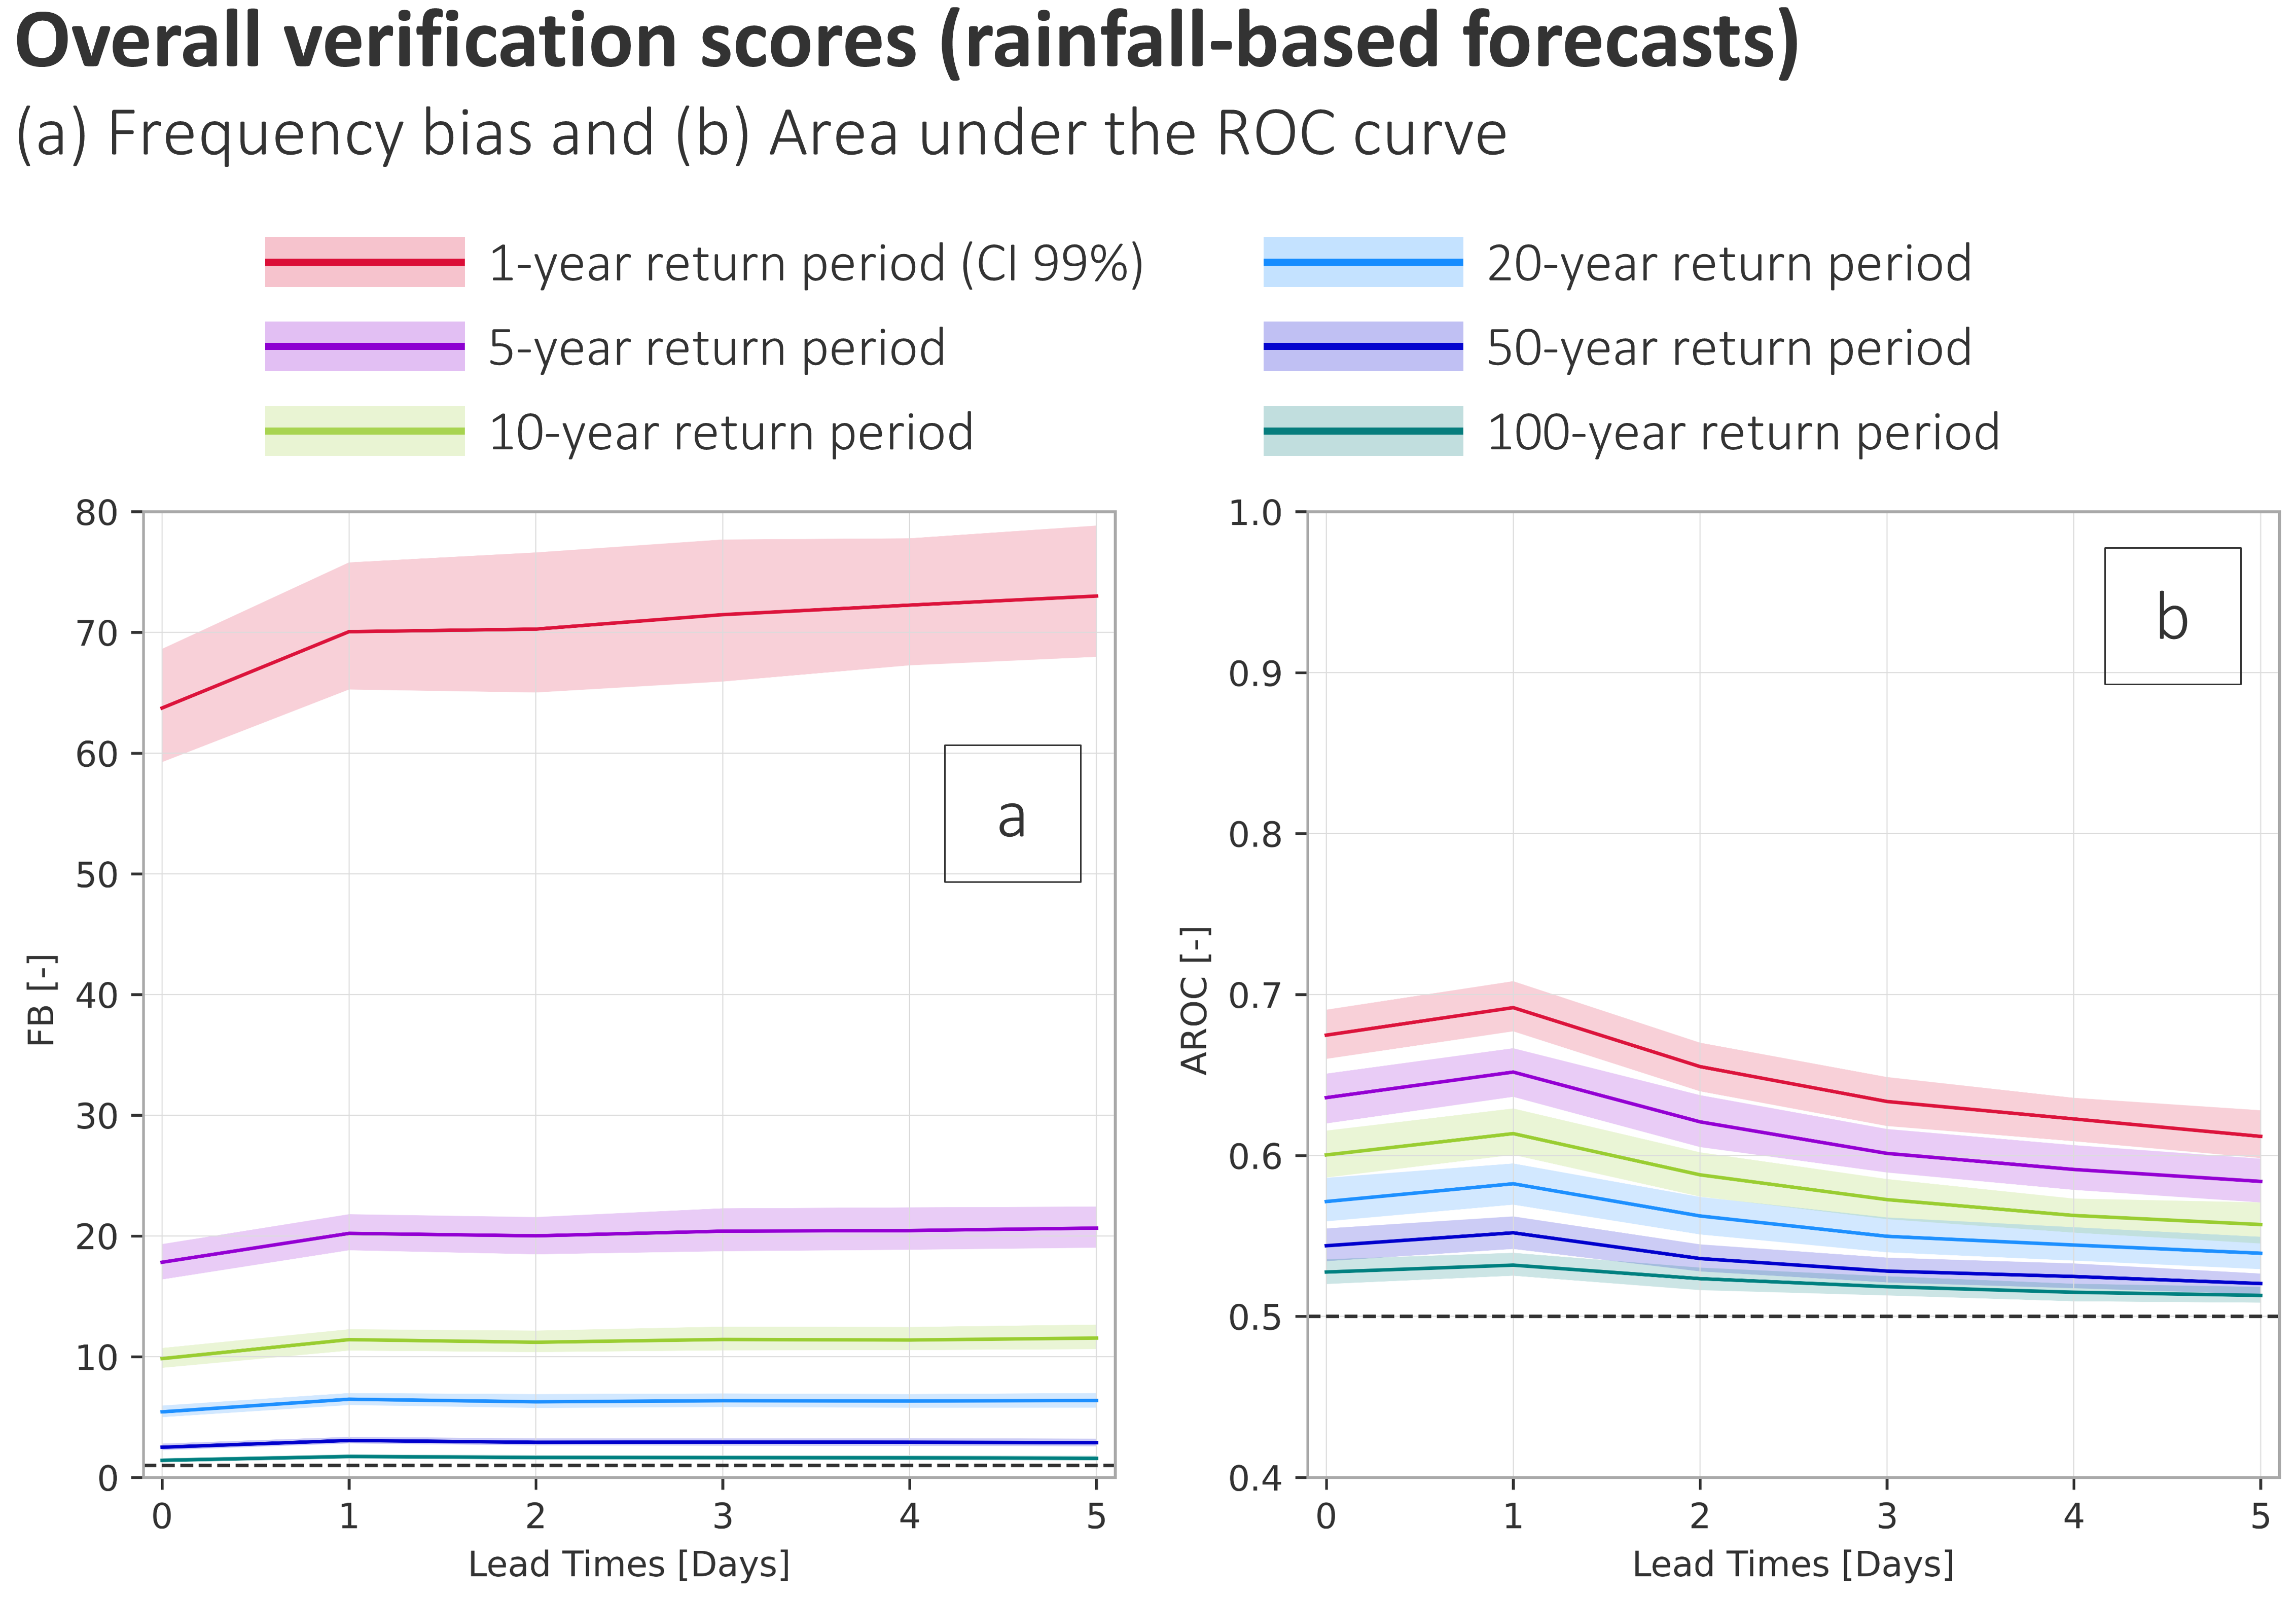
\includegraphics[width=\textwidth]{chapter_05/figures/rainfall_based_ff_verif_overall_scores.png}
\caption{\textbf{Overall verification scores for the rainfall-based forecasts of areas at risk of flash flood.} Panel (a) shows the frequency bias (solid lines) for 1-year (in red), 5-year (in purple), 10-year (in light green), 20-year (in cyan), 50-year (in blue), and 100-year return period (in green). The corresponding shaded areas represent the confidence intervals at 99\% confidence level. The inset box contains a zoomed-in version of the panel to show better the frequency bias values close to 1 (representing perfect bias). Panel (b) shows the area under the ROC curve.}
\label{fig:rainfall_based_ff_verif_overall_scores}
\end{figure}


\subsection{Discrimination ability}

All forecasts for rainfall events exceeding the 1-year return period threshold (Figure \ref{fig:rainfall_based_ff_verif_breakdown_scores_roc_1rp}) exhibit a discrimination ability superior to random chance, as the curves are above the diagonal reference line. A systematic degradation in discrimination ability is observed with increasing lead time, with the Area Under the ROC Curve (AROC) values ranging from 0.675 for the short-range forecasts (Figure \ref{fig:rainfall_based_ff_verif_breakdown_scores_roc_1rp}a) to 0.612 (\sim9\% reduction) for t+120 (day 5, Figure \ref{fig:rainfall_based_ff_verif_breakdown_scores_roc_1rp}f). Despite such a reduction, the forecasts show a good discrimination ability throughout the forecast horizon. Day 1 forecasts (t+24) show a higher discrimination ability than the short-range forecasts, and only from day 2 forecasts (t+48), the discrimination ability of the long-range forecasts goes below that of the reanalysis. The relatively narrow confidence intervals (at 99\% confidence level) suggest that the differences in skill between forecast configurations are statistically meaningful at the considered confidence level.

\begin{figure}[htbp]
\centering
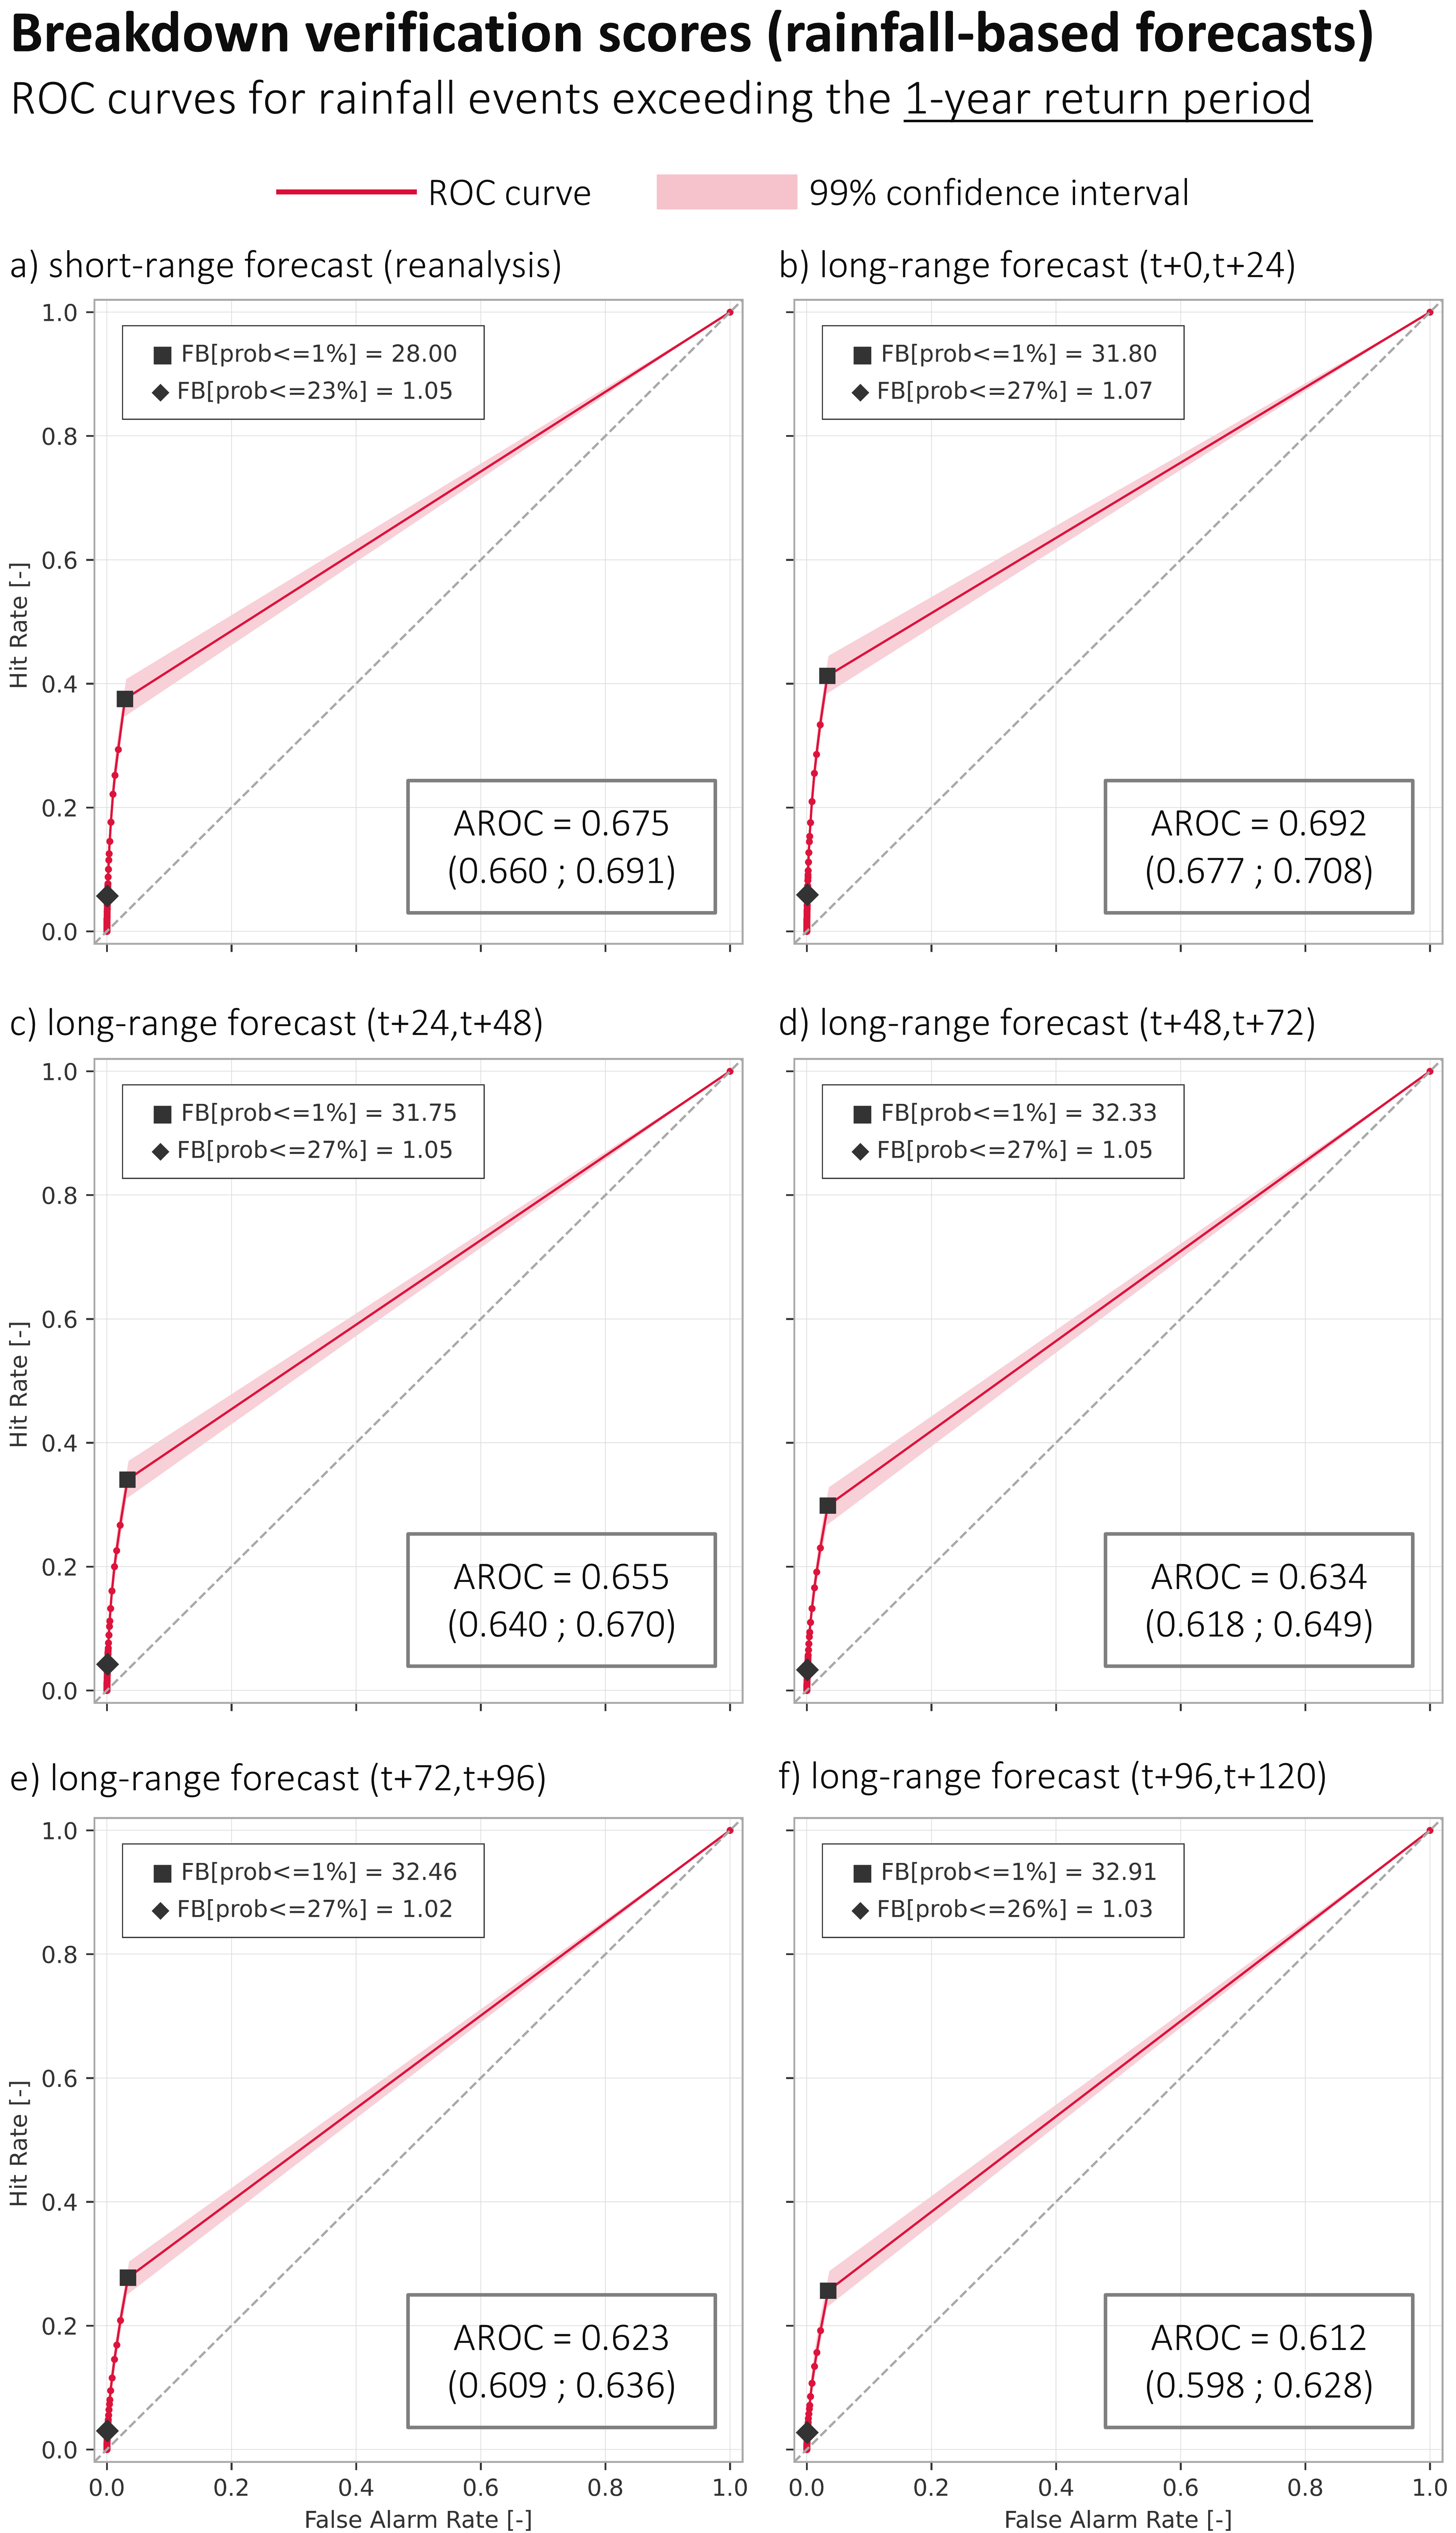
\includegraphics[width=\textwidth]{chapter_05/figures/rainfall_based_ff_verif_breakdown_scores_roc_1rp.png}
\caption{\textbf{ROC curves for tp >= 1-year return period for the rainfall-based forecasts of areas at risk of flash floods built with ERA5-ecPoint.} Panel (a) shows the ROC curve (blue solid line) for the short-range predictions together with the confidence intervals (blue shaded area) at 99\% confidence level. Panels (b) to (f) refer to the long-range forecasts, for accumulation periods ending in t+24, t+48, t+72, t+96, and t+120, respectively. The pink dots refer to the probability threshold at which the frequency bias has the closest value to 1 (i.e., perfectly reliable forecast), while the orange dot shows the value of the frequency bias for the lowest probability threshold available in ERA5-ecPoint (i.e., the 99th percentile).}
\label{fig:rainfall_based_ff_verif_breakdown_scores_roc_1rp}
\end{figure}

The pink dot in Figure \ref{fig:rainfall_based_ff_verif_breakdown_scores_roc_1rp}a shows that perfect reliability (i.e. frequency bias equal to 1) is reach for probabilities <= 23\%. For the long-range forecasts, the probability thresholds at which perfect reliability is achieved is compatible to the short-range, being 27\% for all the lead times except t+120 which is 26\%. The frequency bias for the lowest probability threshold (i.e. 99th percentile or probability threshold equal to 1\%) in the short-range forecasts equals to 28. The frequency biases for the long-range forecasts are similar, falling between 31 and 33. 

Similar results are obtained for the 5-, 10-, 20-, 50-, and 100-year return periods.

\begin{figure}[htbp]
\centering
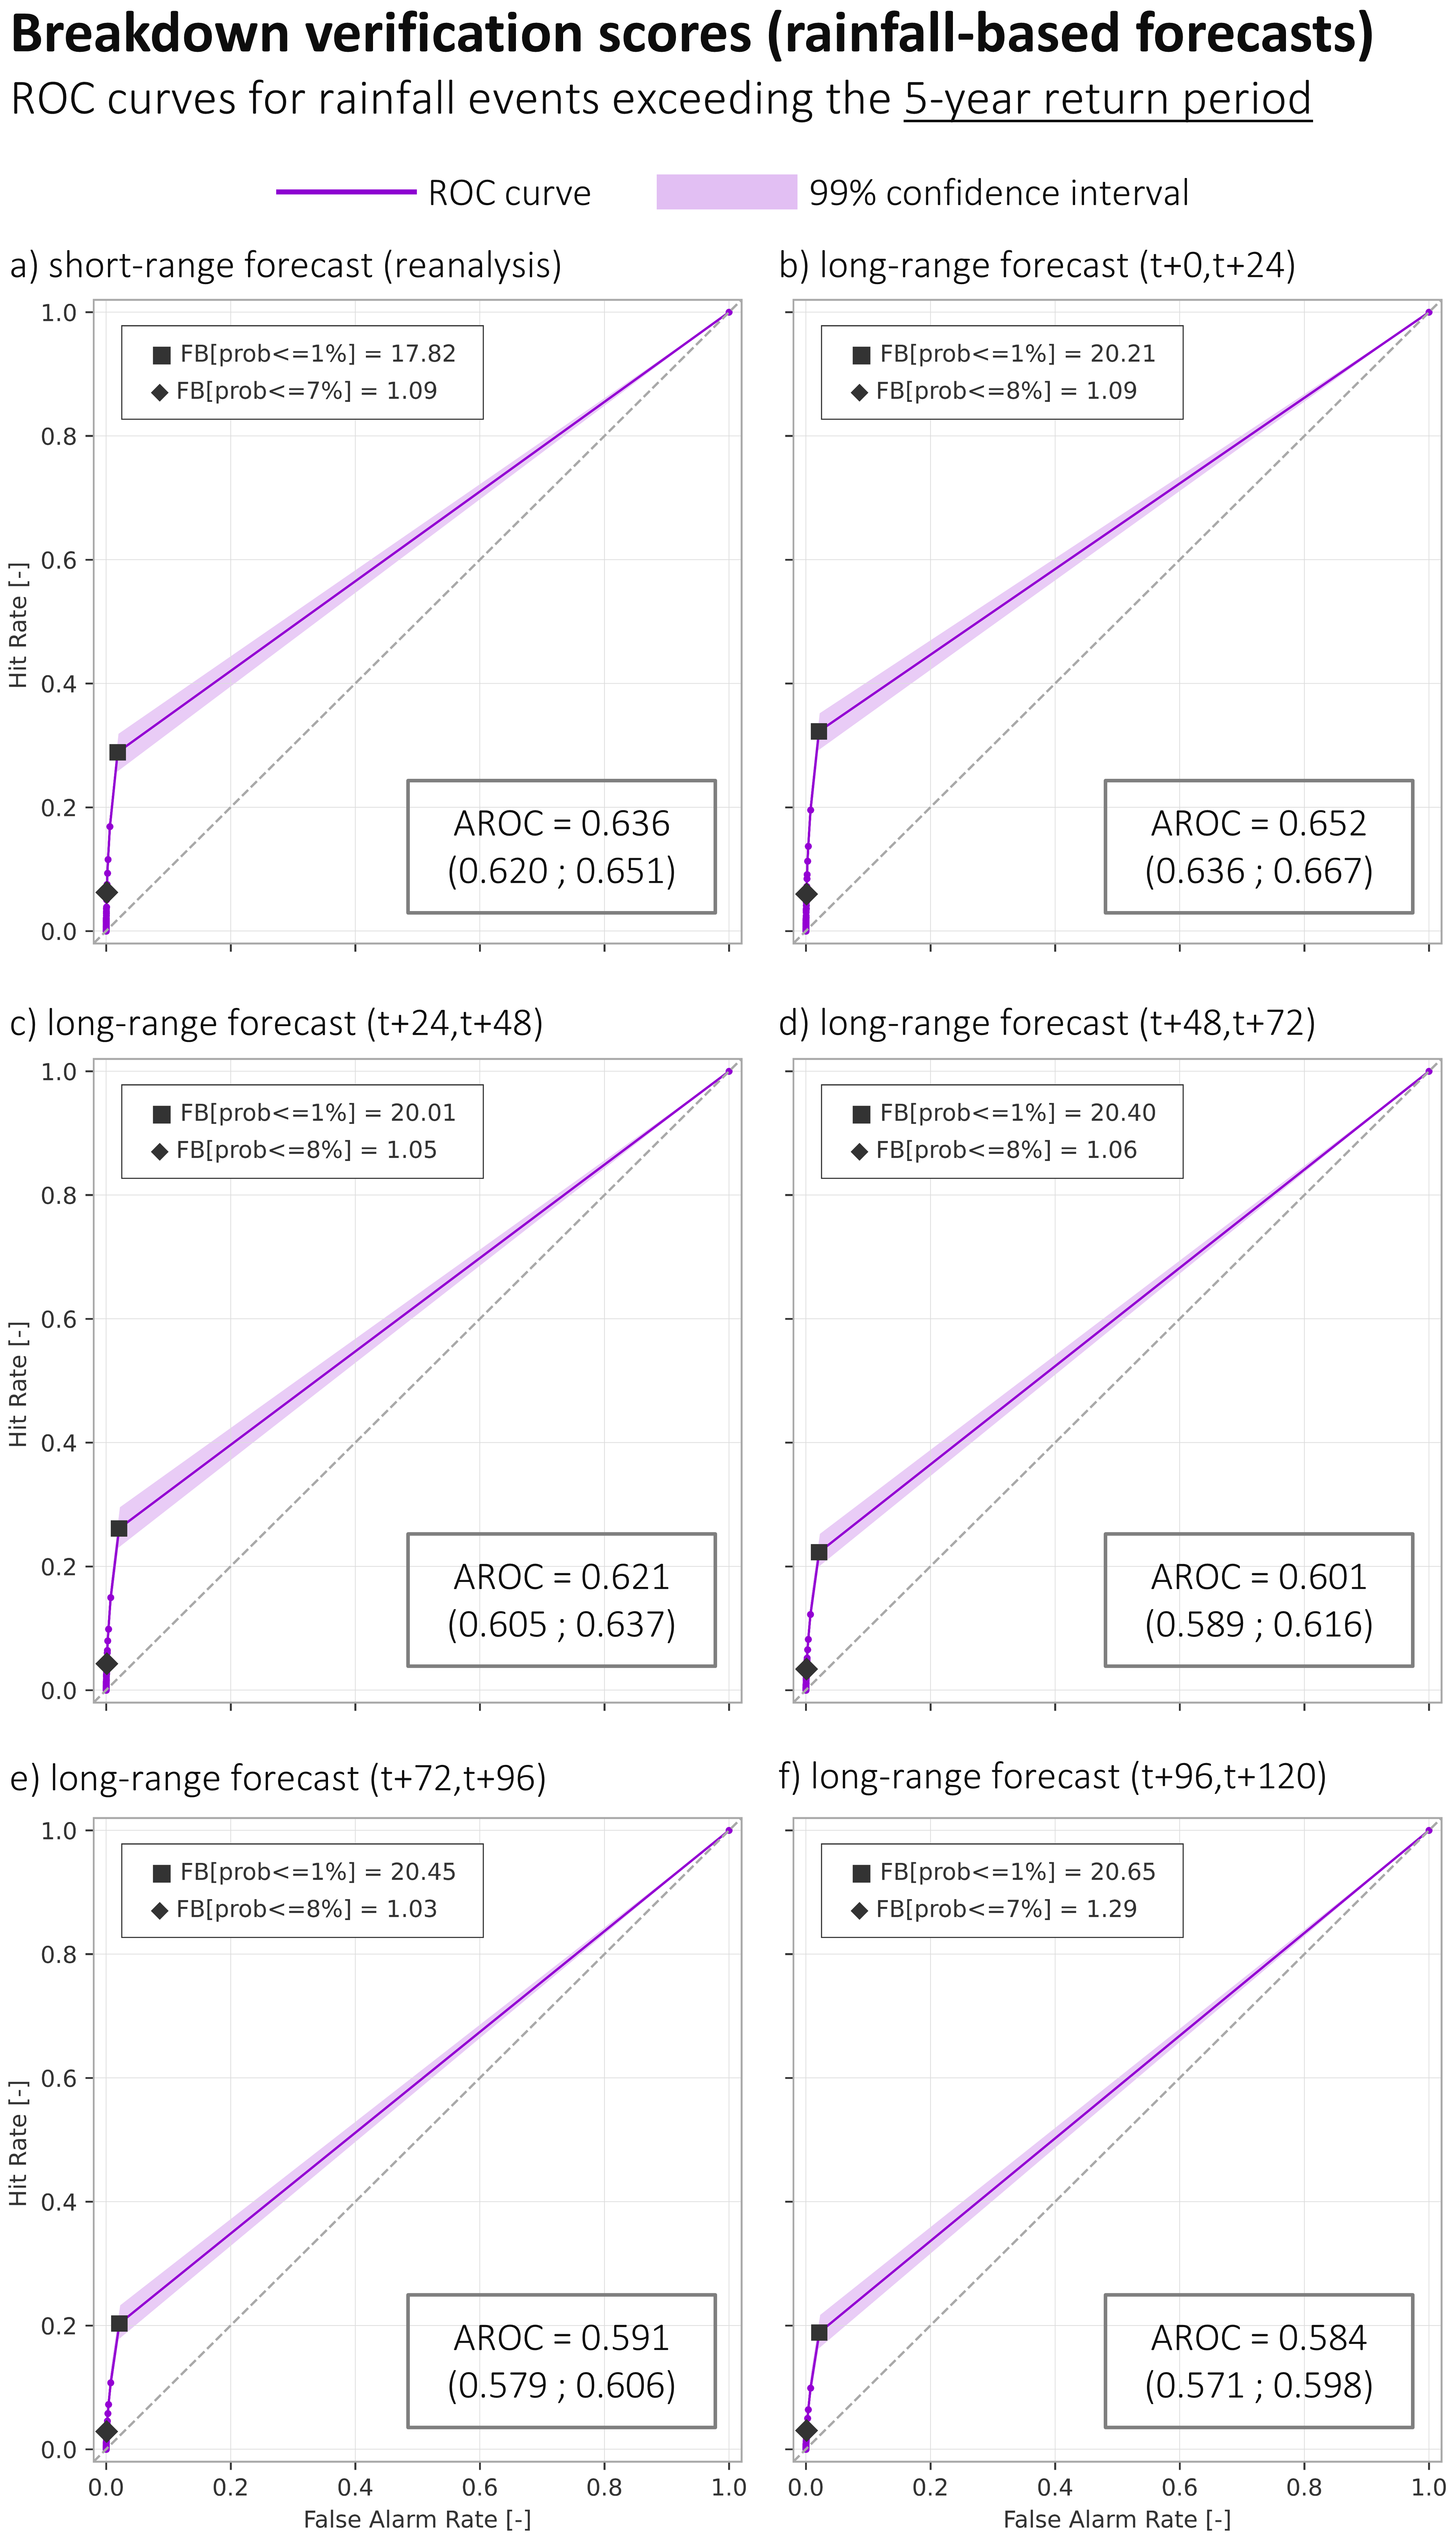
\includegraphics[width=\textwidth]{chapter_05/figures/rainfall_based_ff_verif_breakdown_scores_roc_5rp.png}
\caption{\textbf{ROC curves for tp >= 5-year return period for the rainfall-based forecasts of areas at risk of flash floods built with ERA5-ecPoint.} Similar to Figure \ref{fig:rainfall_based_ff_verif_breakdown_scores_roc_1rp}.}
\label{fig:rainfall_based_ff_verif_breakdown_scores_roc_5rp}
\end{figure}

\begin{figure}[htbp]
\centering
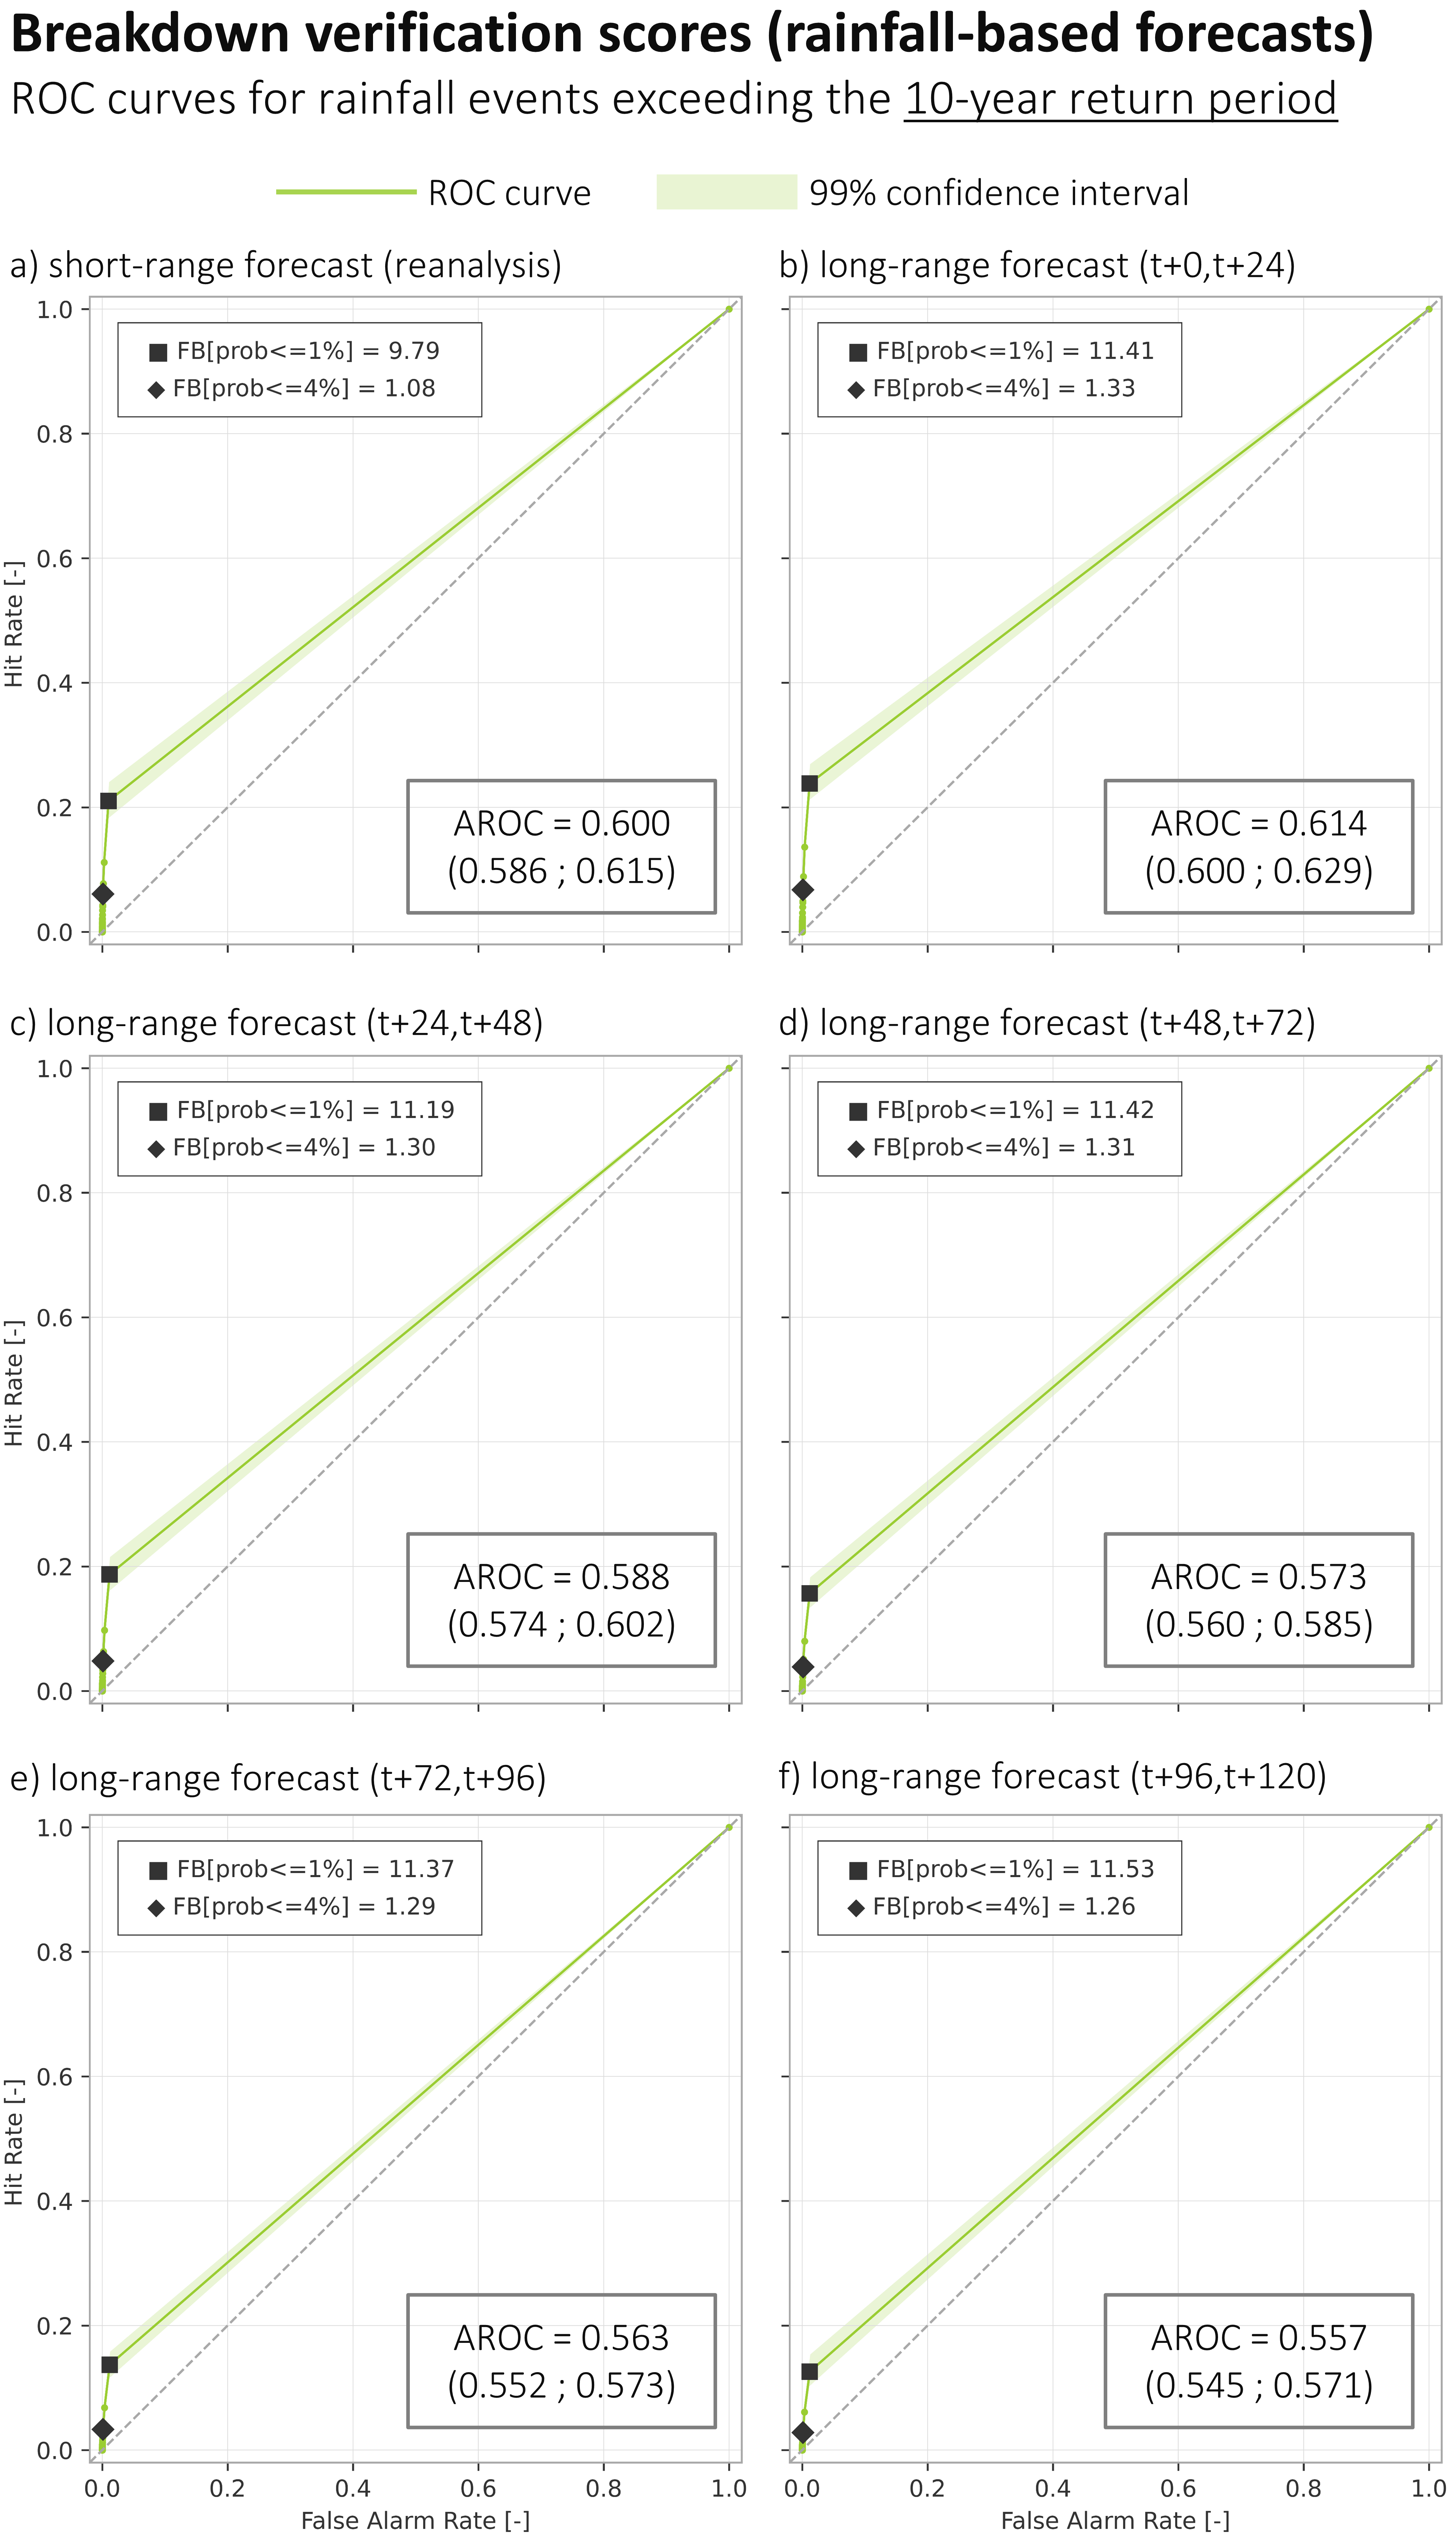
\includegraphics[width=\textwidth]{chapter_05/figures/rainfall_based_ff_verif_breakdown_scores_roc_10rp.png}
\caption{\textbf{ROC curves for tp >= 10-year return period for the rainfall-based forecasts of areas at risk of flash floods built with ERA5-ecPoint.} Similar to Figure \ref{fig:rainfall_based_ff_verif_breakdown_scores_roc_1rp}.}
\label{fig:rainfall_based_ff_verif_breakdown_scores_roc_10rp}
\end{figure}

\begin{figure}[htbp]
\centering
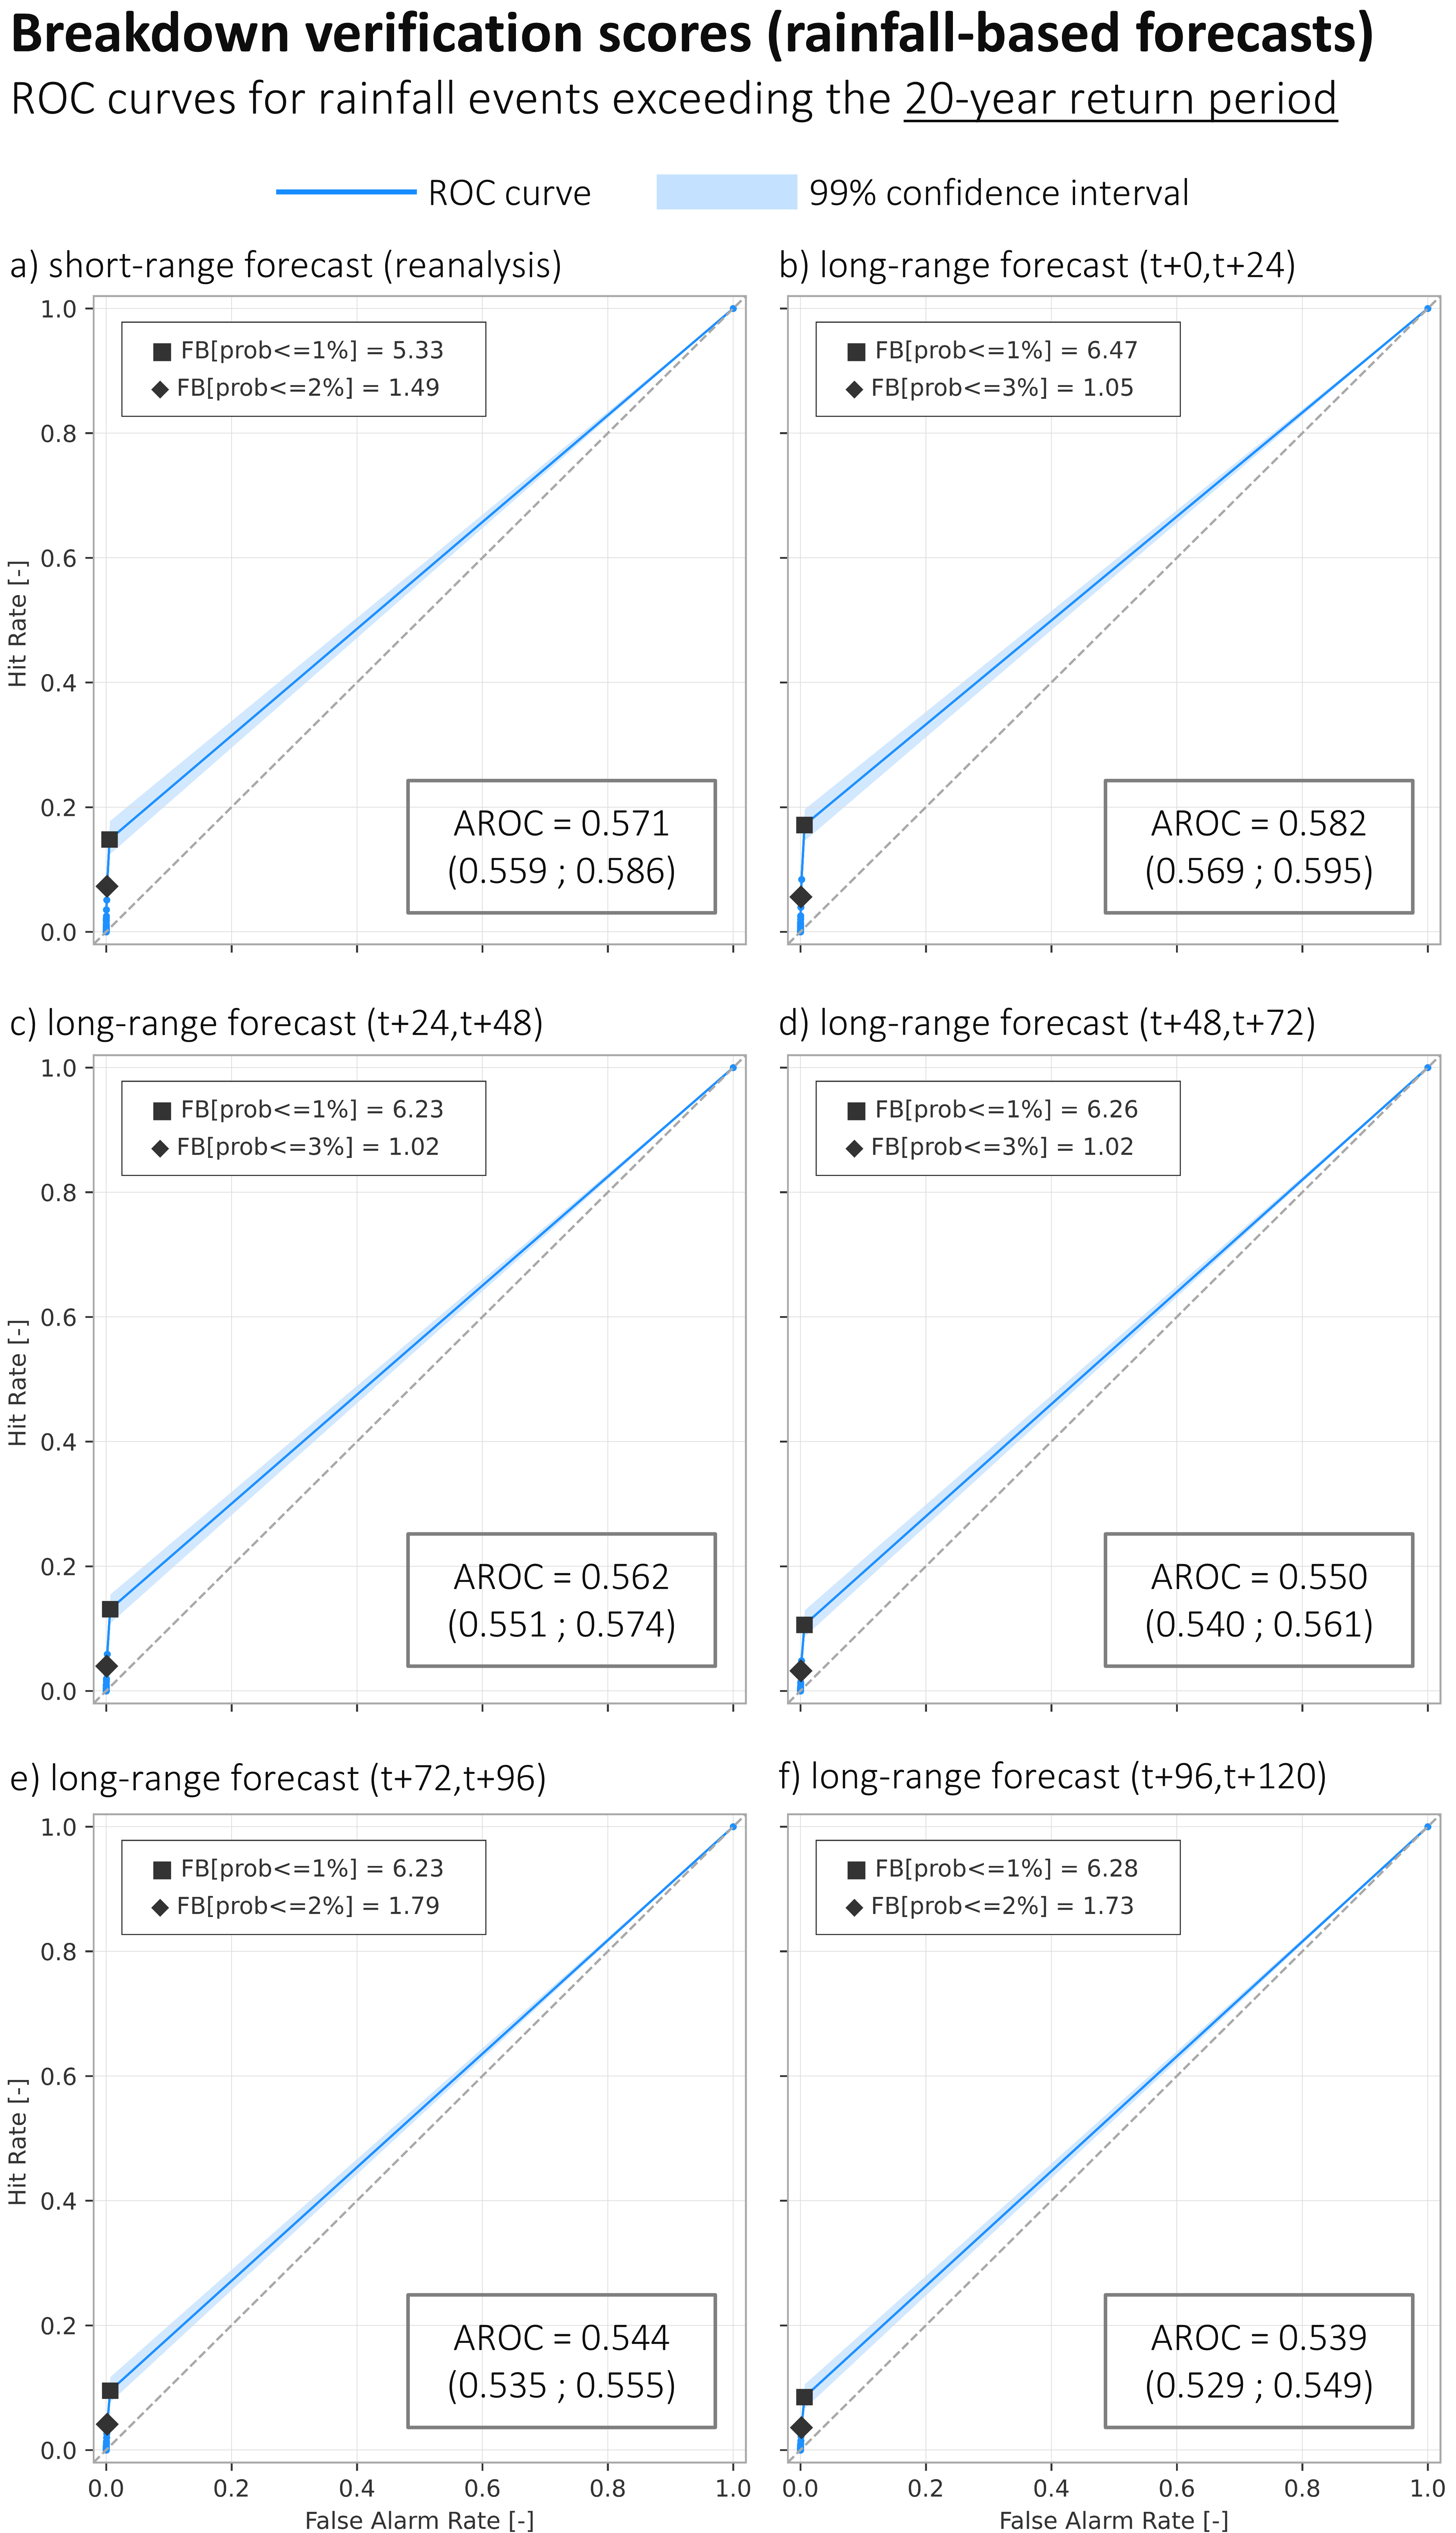
\includegraphics[width=\textwidth]{chapter_05/figures/rainfall_based_ff_verif_breakdown_scores_roc_20rp.png}
\caption{\textbf{ROC curves for tp >= 20-year return period for the rainfall-based forecasts of areas at risk of flash floods built with ERA5-ecPoint.} Similar to Figure \ref{fig:rainfall_based_ff_verif_breakdown_scores_roc_1rp}.}
\label{fig:rainfall_based_ff_verif_breakdown_scores_roc_20rp}
\end{figure}

\begin{figure}[htbp]
\centering
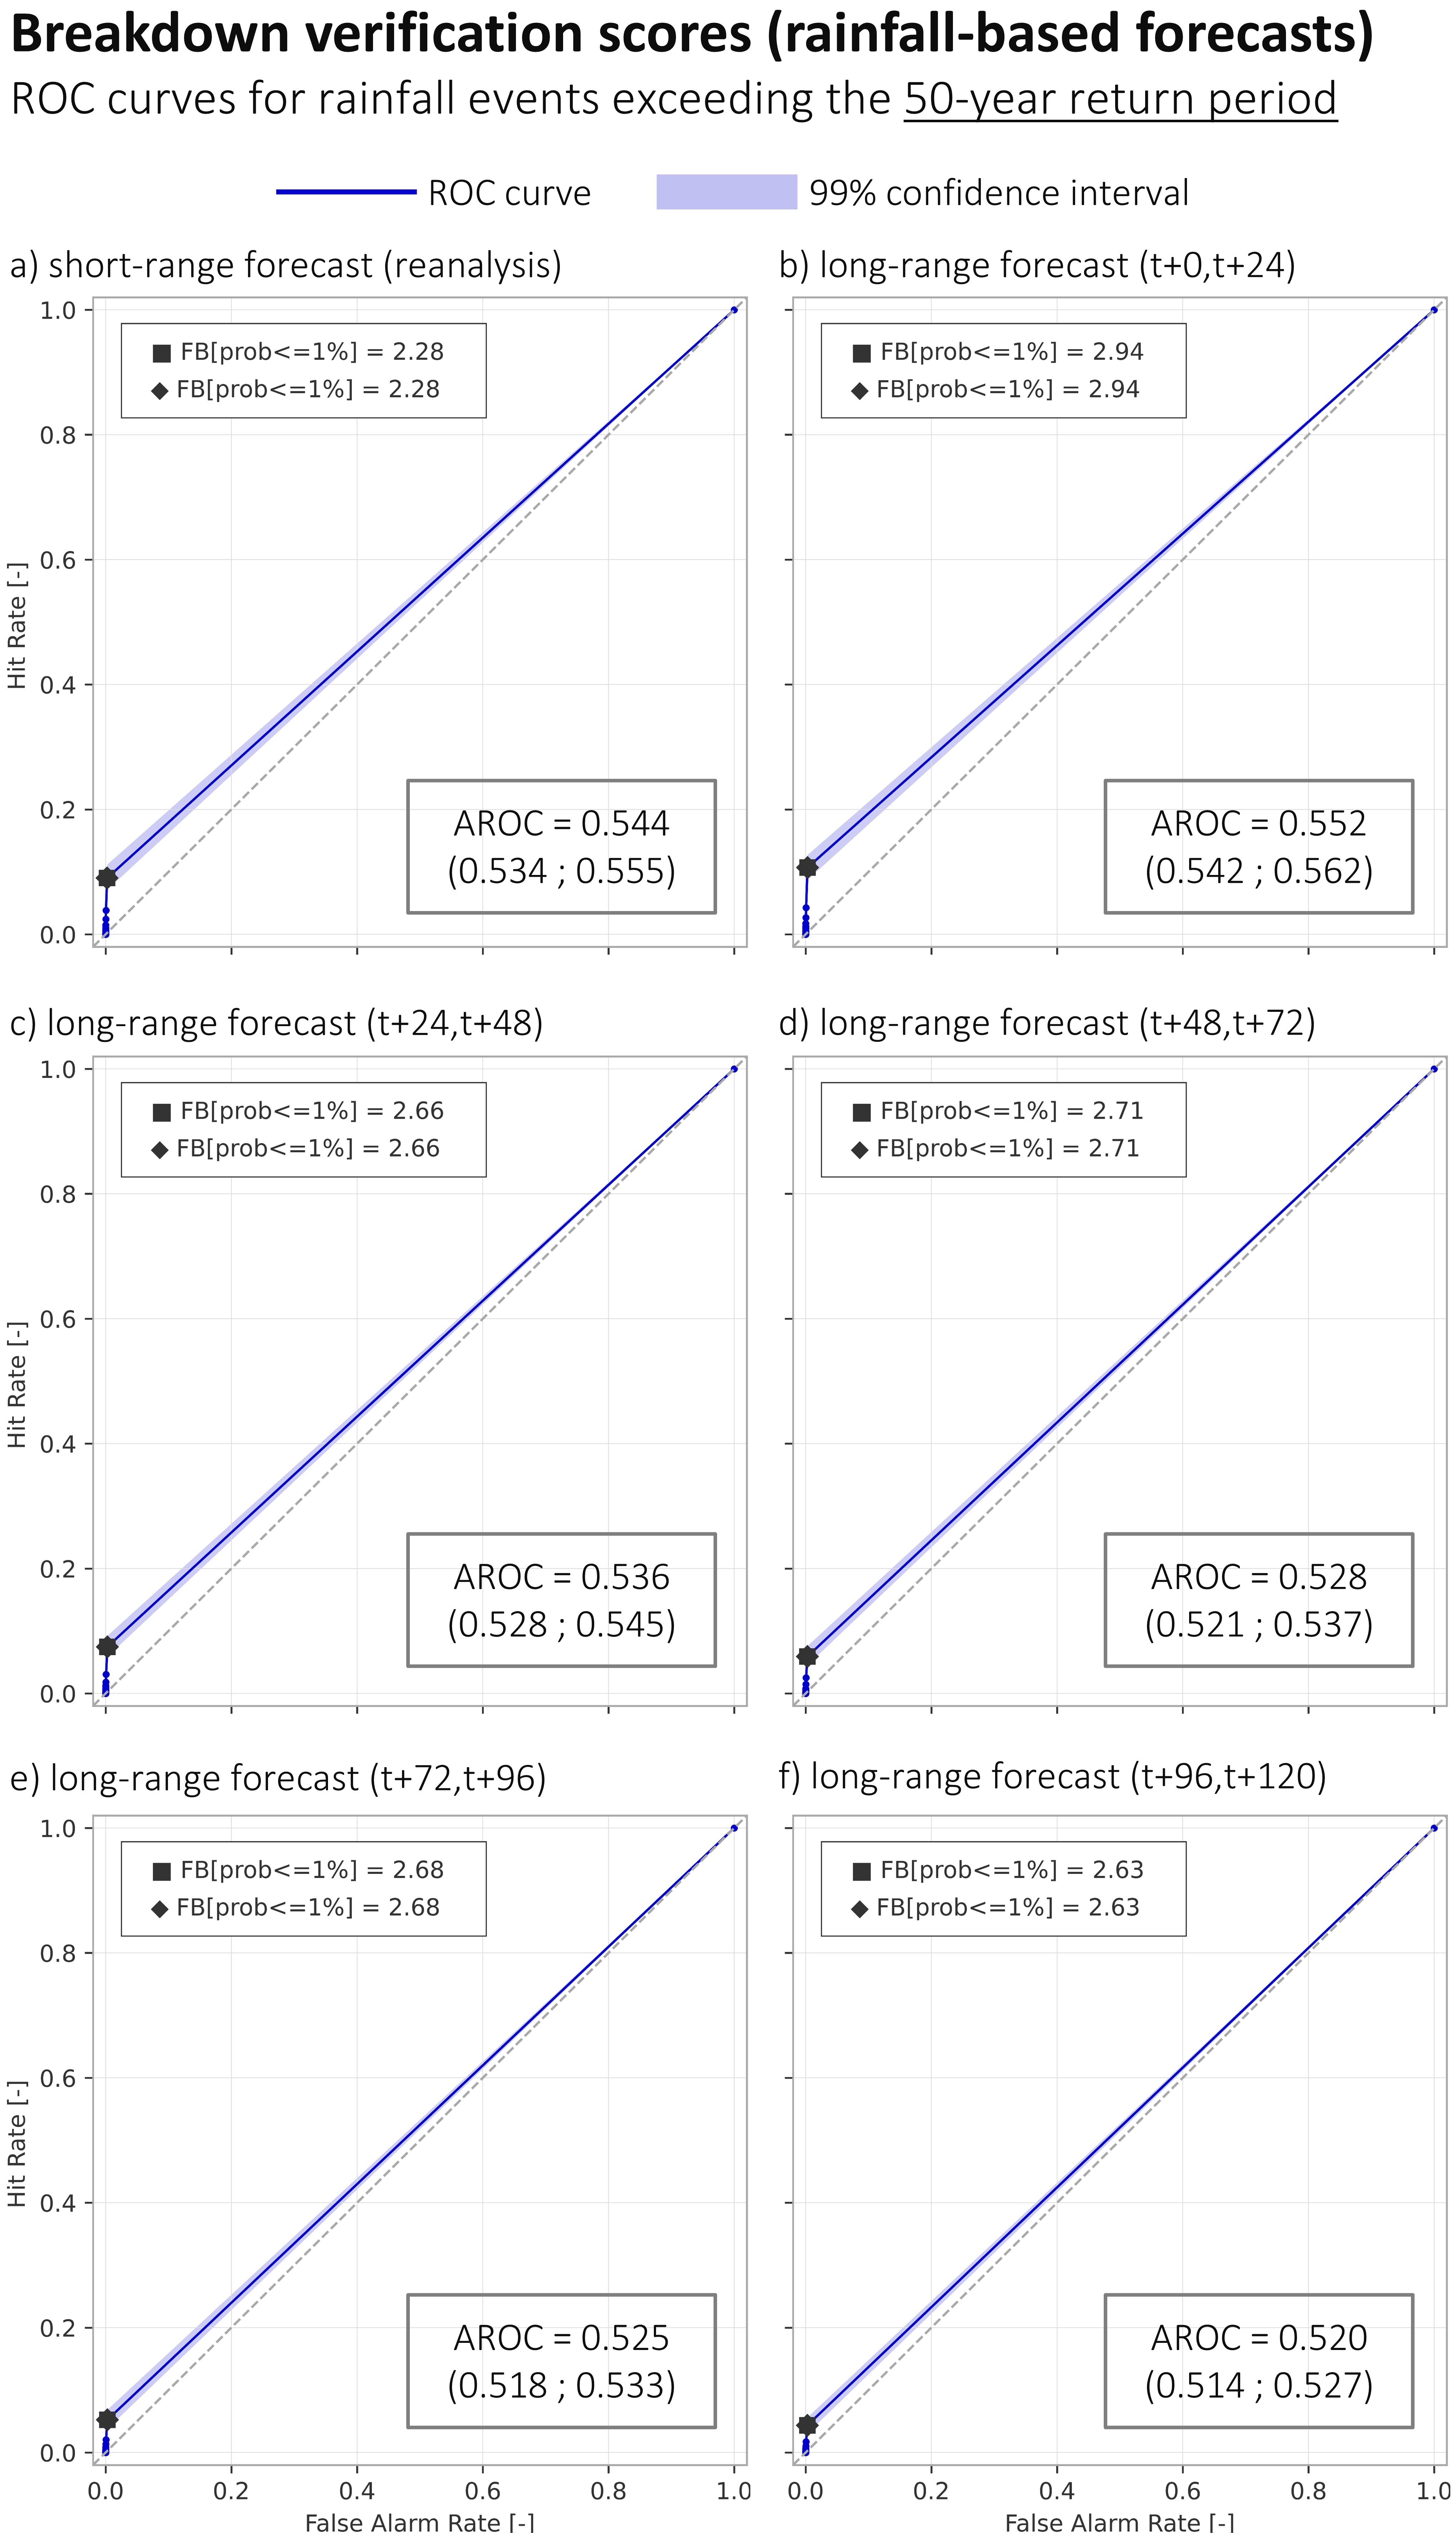
\includegraphics[width=\textwidth]{chapter_05/figures/rainfall_based_ff_verif_breakdown_scores_roc_50rp.png}
\caption{\textbf{ROC curves for tp >= 50-year return period for the rainfall-based forecasts of areas at risk of flash floods built with ERA5-ecPoint.} Similar to Figure \ref{fig:rainfall_based_ff_verif_breakdown_scores_roc_1rp}.}
\label{fig:rainfall_based_ff_verif_breakdown_scores_roc_50rp}
\end{figure}

\begin{figure}[htbp]
\centering
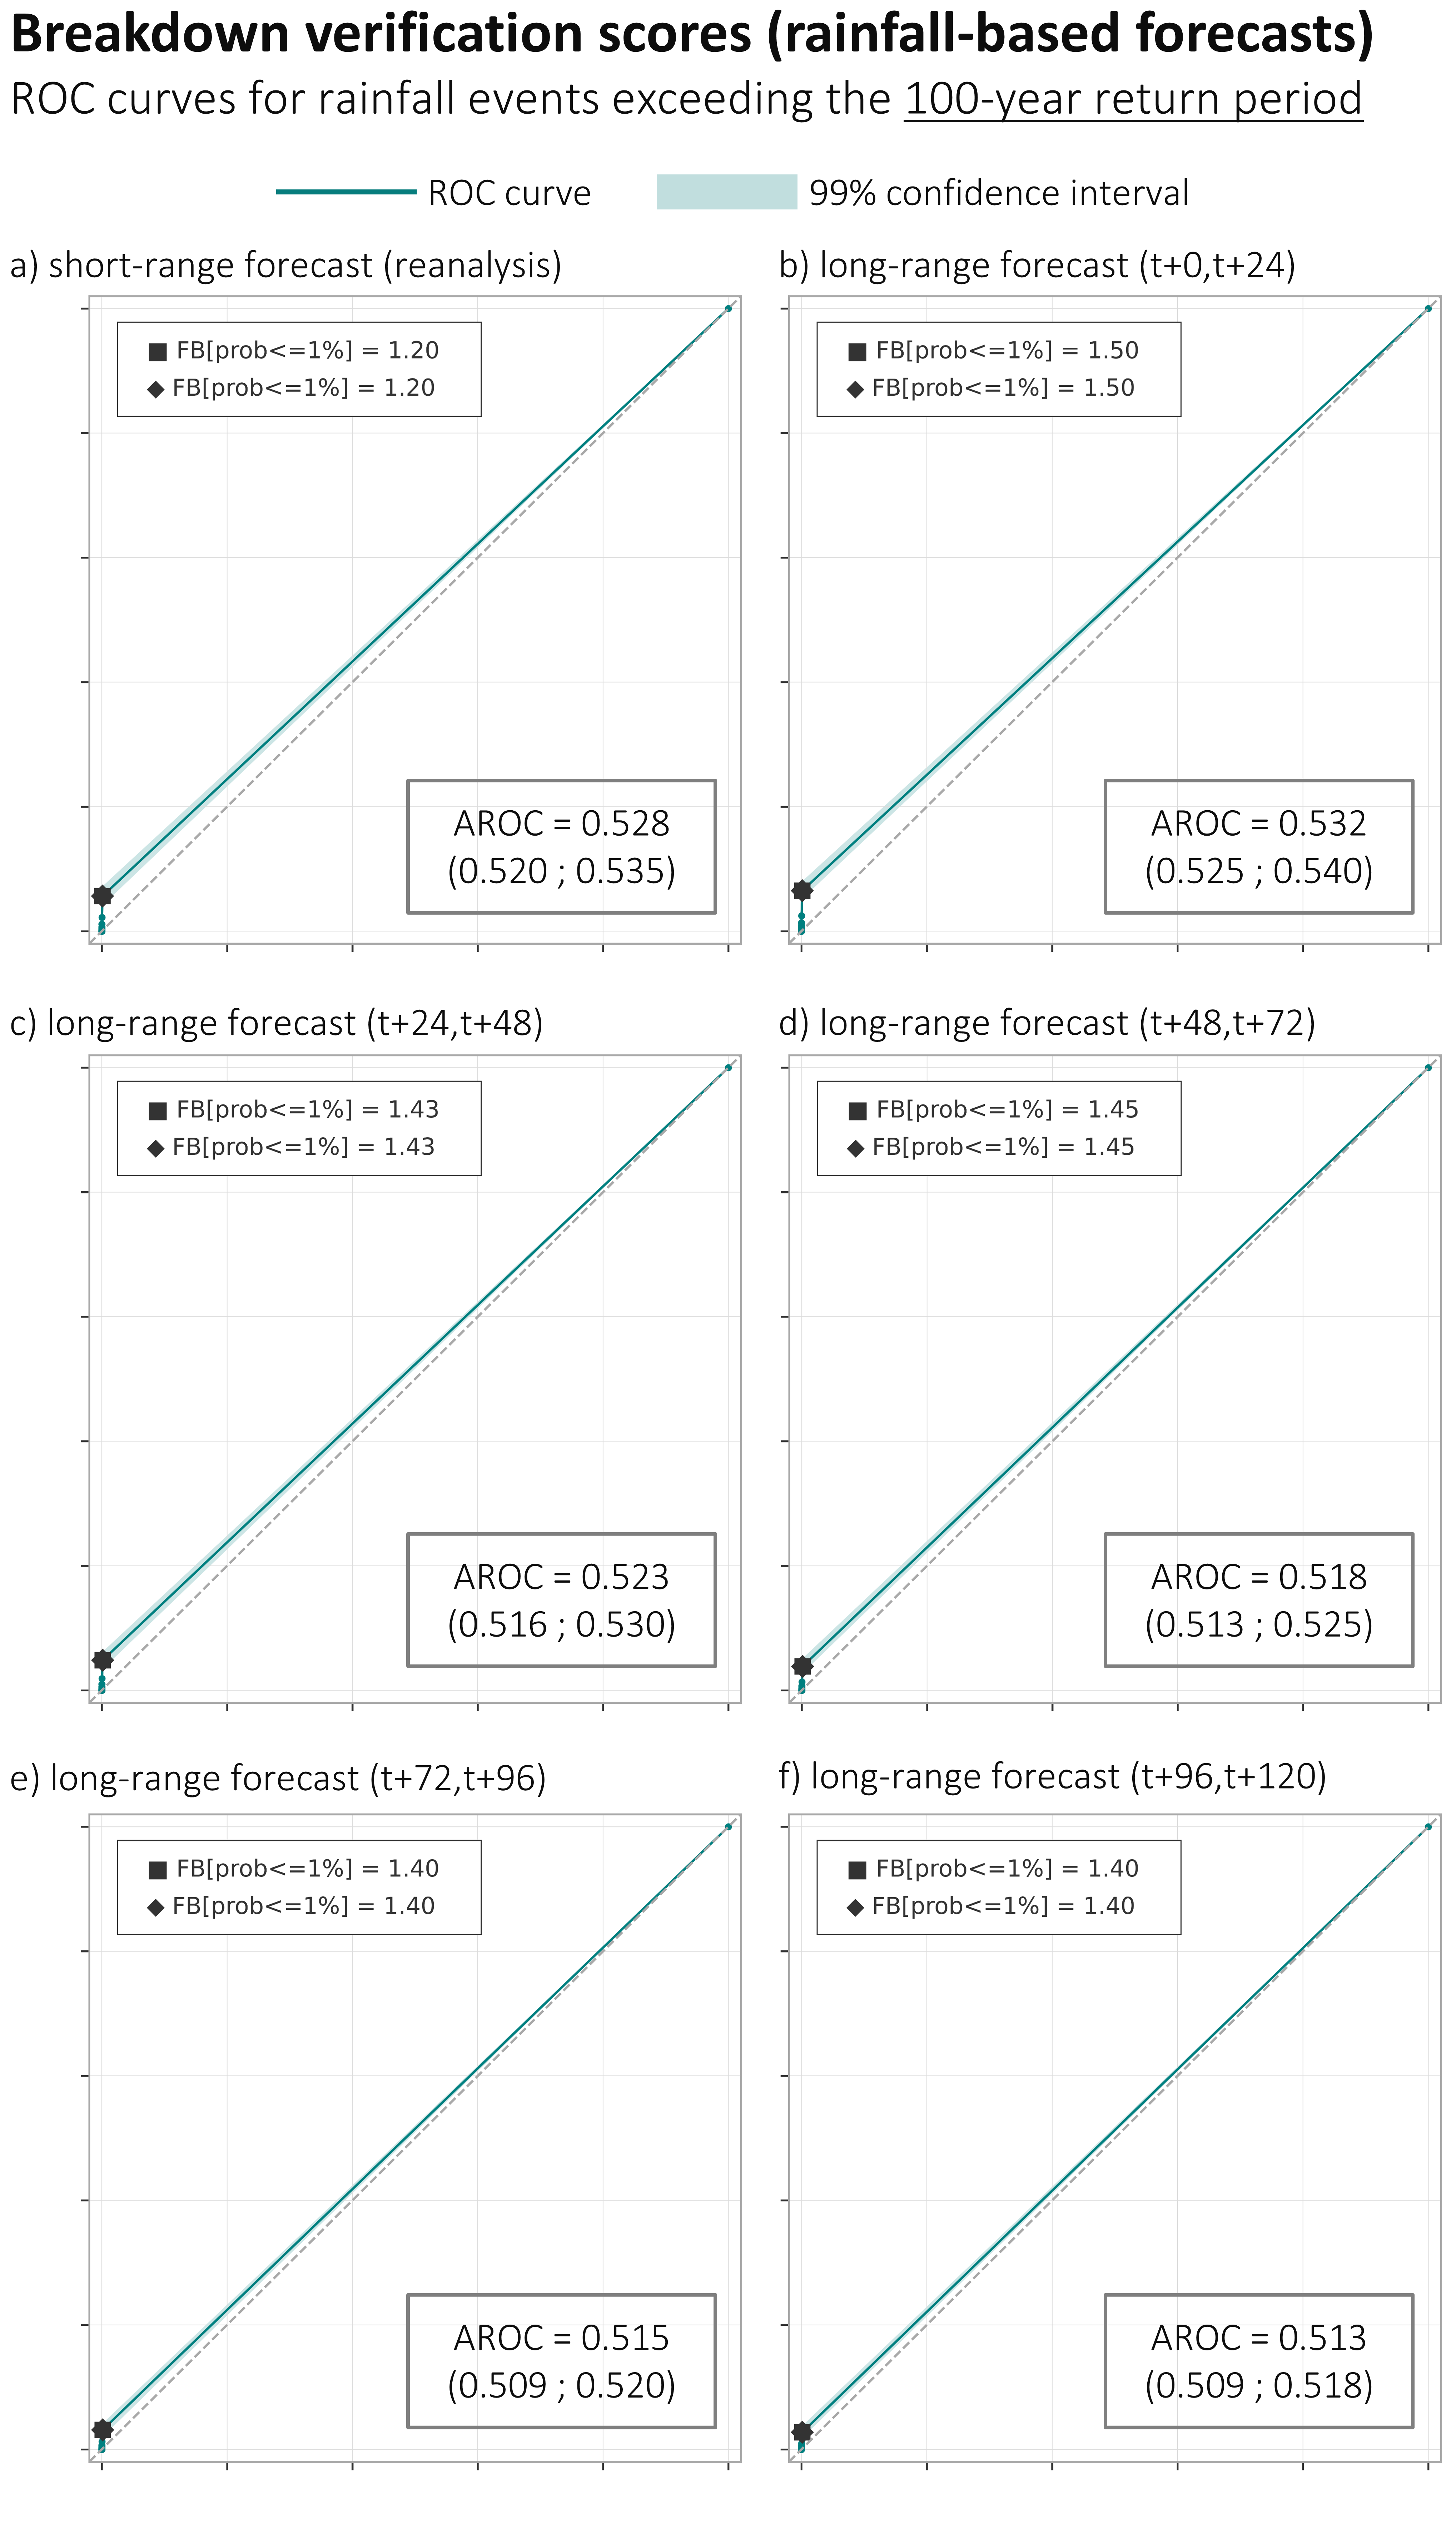
\includegraphics[width=\textwidth]{chapter_05/figures/rainfall_based_ff_verif_breakdown_scores_roc_100rp.png}
\caption{\textbf{ROC curves for tp >= 100-year return period for the rainfall-based forecasts of areas at risk of flash floods built with ERA5-ecPoint.} Similar to Figure \ref{fig:rainfall_based_ff_verif_breakdown_scores_roc_1rp}.}
\label{fig:rainfall_based_ff_verif_breakdown_scores_roc_100rp}
\end{figure}


\subsection{Reliability}

All forecasts for rainfall events exceeding the 1-year return period threshold (Figure \ref{fig:rainfall_based_ff_verif_breakdown_scores_rel_diag_1rp}) exhibit a systematic overprediction across all lead times, as shown by the reliability diagram being below the diagonal line. This indicates that when the model predicts a given probability, the observed frequency of flash flood events is consistently lower. For example, when the forecasts indicate a 50\% chance of having a flash flood event, the observed frequency ranges from \sim10\% in the short-range forecasts (Figure \ref{fig:rainfall_based_ff_verif_breakdown_scores_rel_diag_1rp}a), and between 10\% (for t+24, Figure \ref{fig:rainfall_based_ff_verif_breakdown_scores_rel_diag_1rp}b) and 2\% (t+120, Figure \ref{fig:rainfall_based_ff_verif_breakdown_scores_rel_diag_1rp}f) in the long-range forecasts. As seen in the ROC curves, the confidence intervals at 99\% are fairly narrow, suggesting that the differences between the reliability diagrams at different lead times are significant at the considered confidence level. However, the confidence levels increase with increasing forecast probabilities. As seen in the corresponding sharpness diagrams (inset boxes in all panels of Figure \ref{fig:rainfall_based_ff_verif_breakdown_scores_rel_diag_1rp}), such widening of the confidence intervals is likely due to the low number of forecasts issued with probabilities higher than ~25\% (when the total number of instances lies below 1000 samples). Such predominance of low probability forecasts suggests that the model (ERA5-ecPoint) rarely expresses high confidence in extreme event occurrence. A notable characteristic of all the reliability diagrams in the Figure \ref{fig:rainfall_based_ff_verif_breakdown_scores_rel_diag_1rp} is the sharp increase in observed frequency for the highest probability bins (i.e. 80\% to 100\%). This steep rise suggests that when the model does issue high probability forecasts, these correspond to genuinely extreme events, though such forecasts remain infrequent.

\begin{figure}[htbp]
\centering
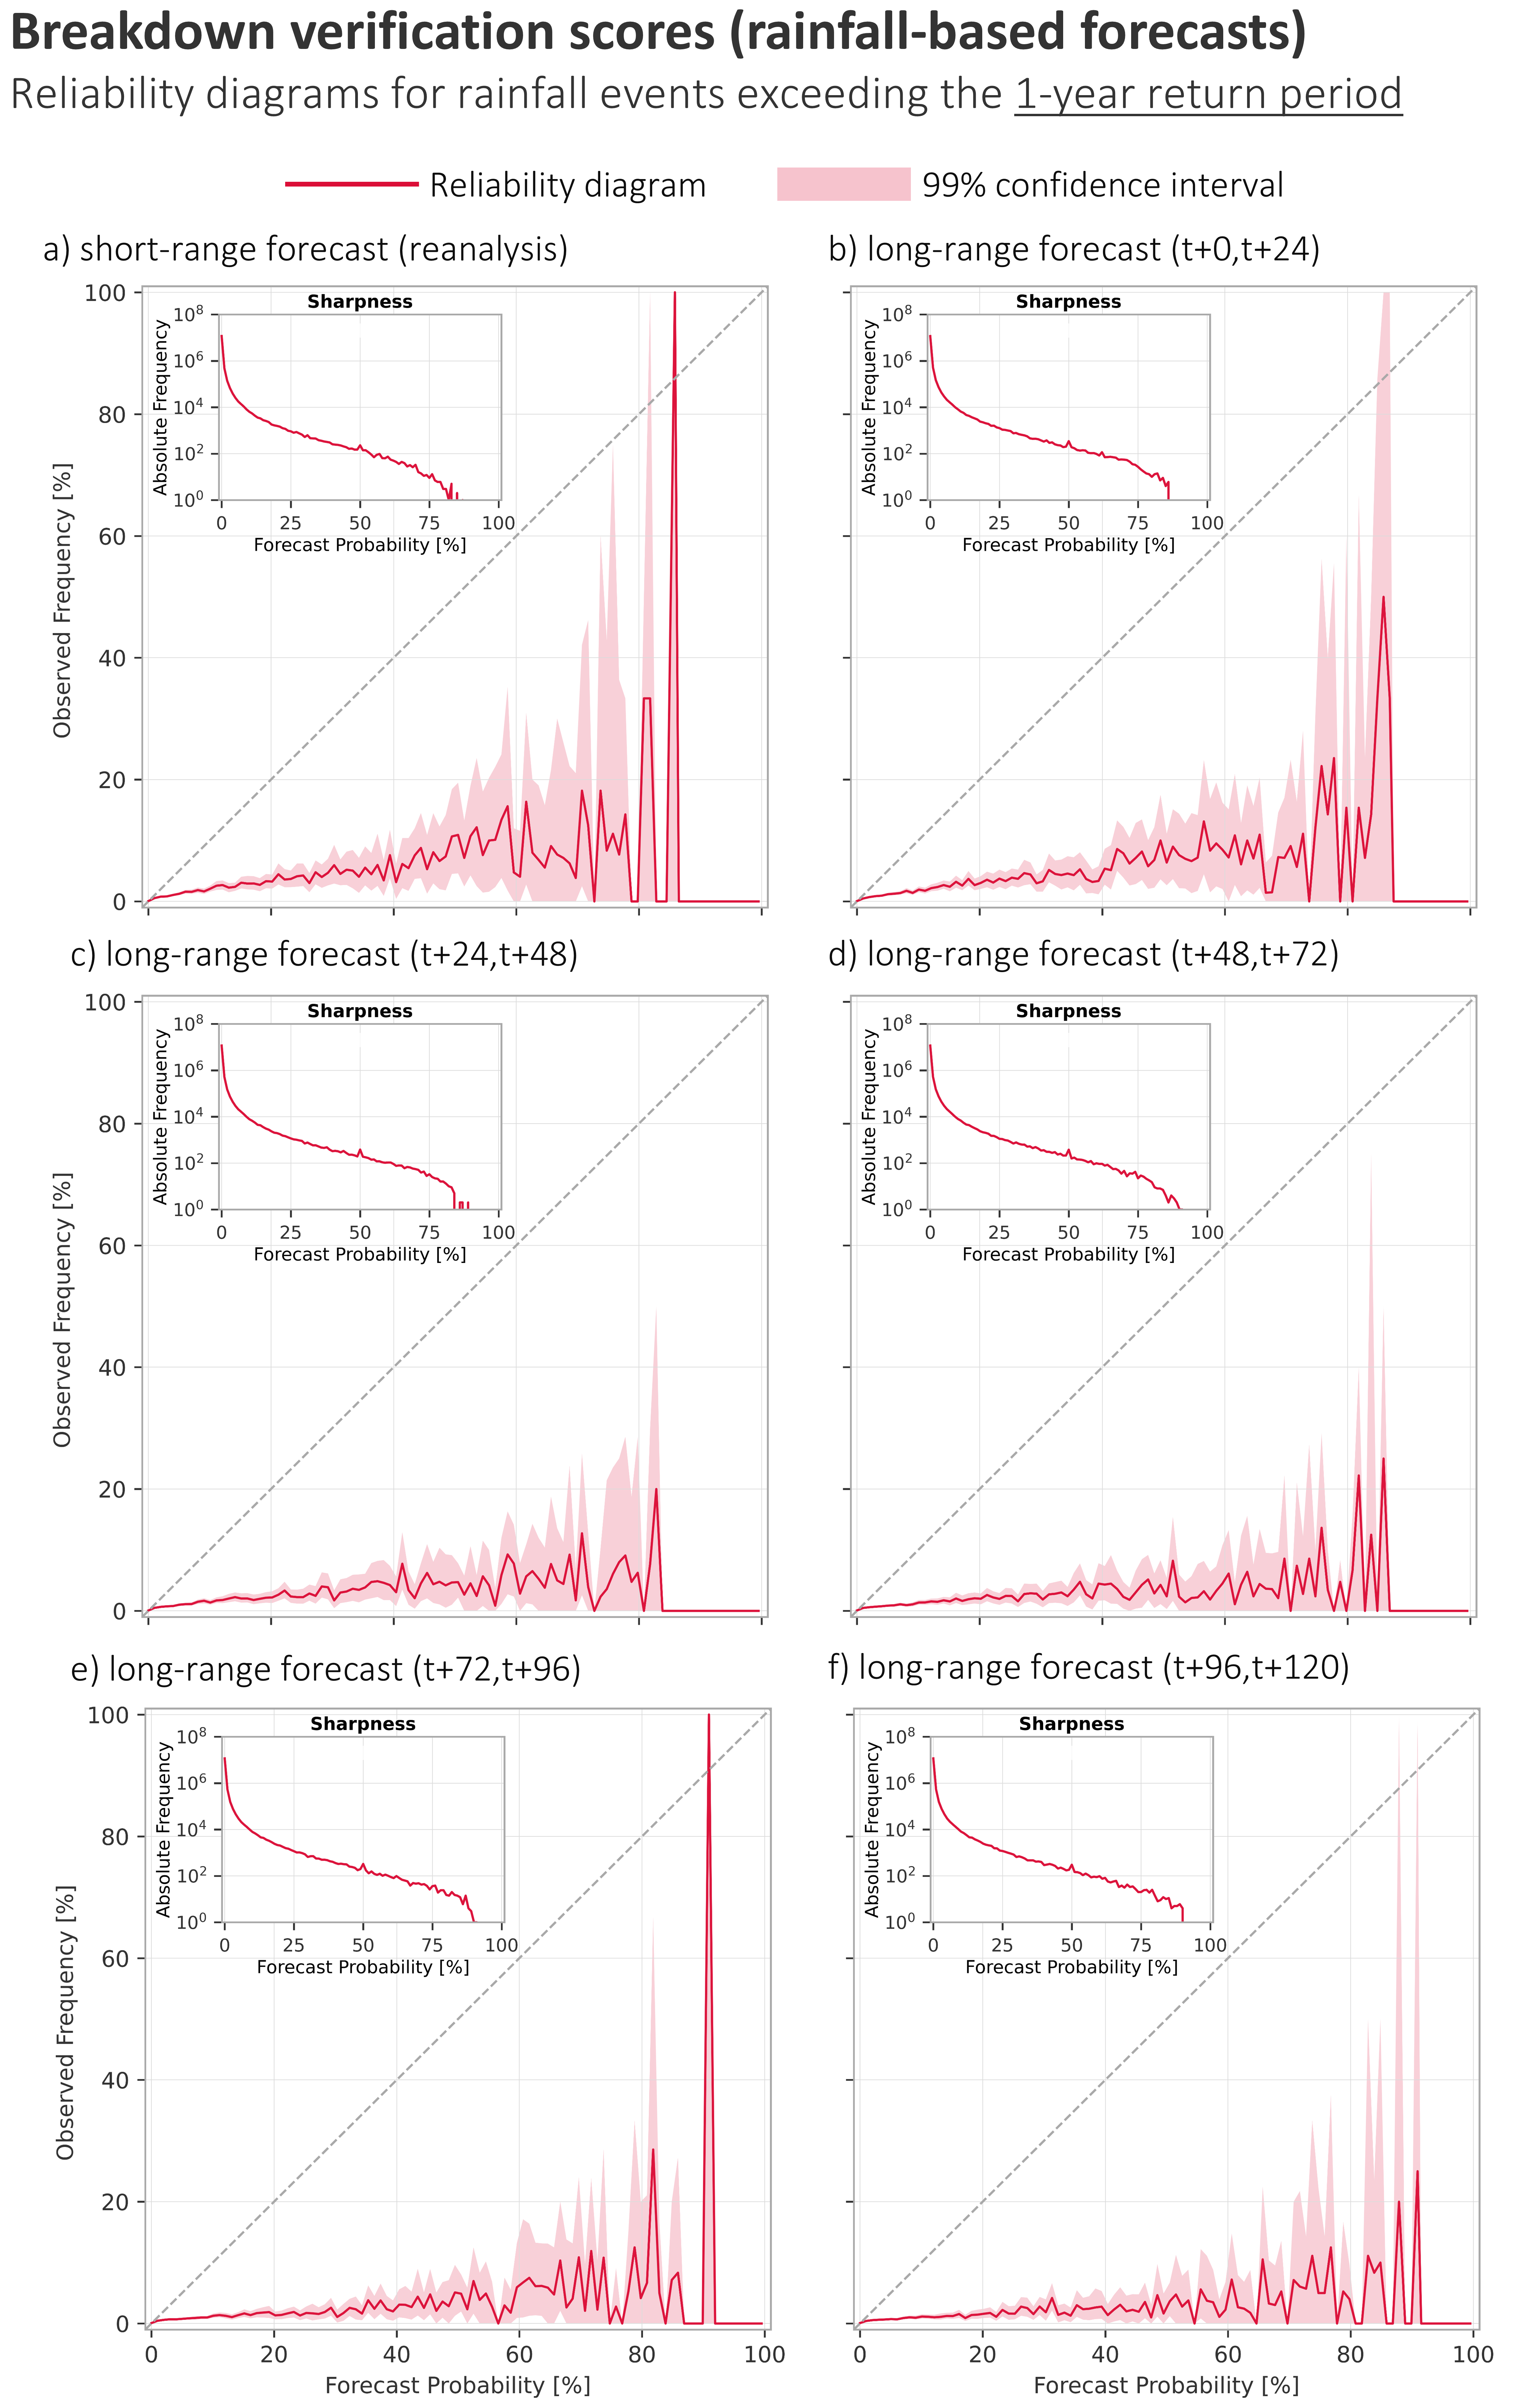
\includegraphics[width=\textwidth]{rainfall_based_ff_verif_breakdown_scores_rel_diag_1rp.png}
\caption{\textbf{Reliability diagrams for tp >= 1-year return period for the rainfall-based forecasts of areas at risk of flash floods built with ERA5-ecPoint.} Panel (a) shows the reliability diagram (blue solid line) for the short-range predictions together with the confidence intervals (blue shaded area) at 99\% confidence level. Panels (b) to (f) refer to the long-range forecasts for accumulation periods ending in t+24, t+48, t+72, t+96, and t+120, respectively. The inset boxes show the corresponding sharpness diagrams.}
\label{fig:rainfall_based_ff_verif_breakdown_scores_rel_diag_1rp}
\end{figure}

The temporal evolution from Figure \ref{fig:rainfall_based_ff_verif_breakdown_scores_rel_diag_1rp}a to f reveals subtle changes in the forecasts' reliability characteristics with increasing lead time. Whilst the general pattern of overprediction persists, from day 2 forecasts (t+48) results more squashed into a flat line over very small observed frequencies, indicating that even though the model issues forecasts with high probabilities of exceeding the 1-year return period at longer lead times with a similar frequency of the short-range forecasts and the day 1 (t+24) long-range forecast, such forecasts do not necessarily correspond to an observed flash flood event.

The reliability diagrams get closer to the diagonal line (indicating perfect bias) as we increase the rainfall threshold to identify the flash flood events. Perfect reliability is observed for rainfall events exceeding the 10-, 20-year, and 50-year return period with probabilities below 5\% at day 1 forecast (t+24) for the 10-, 20-year return period, and 10\% for the 50-year return period.

\begin{figure}[htbp]
\centering
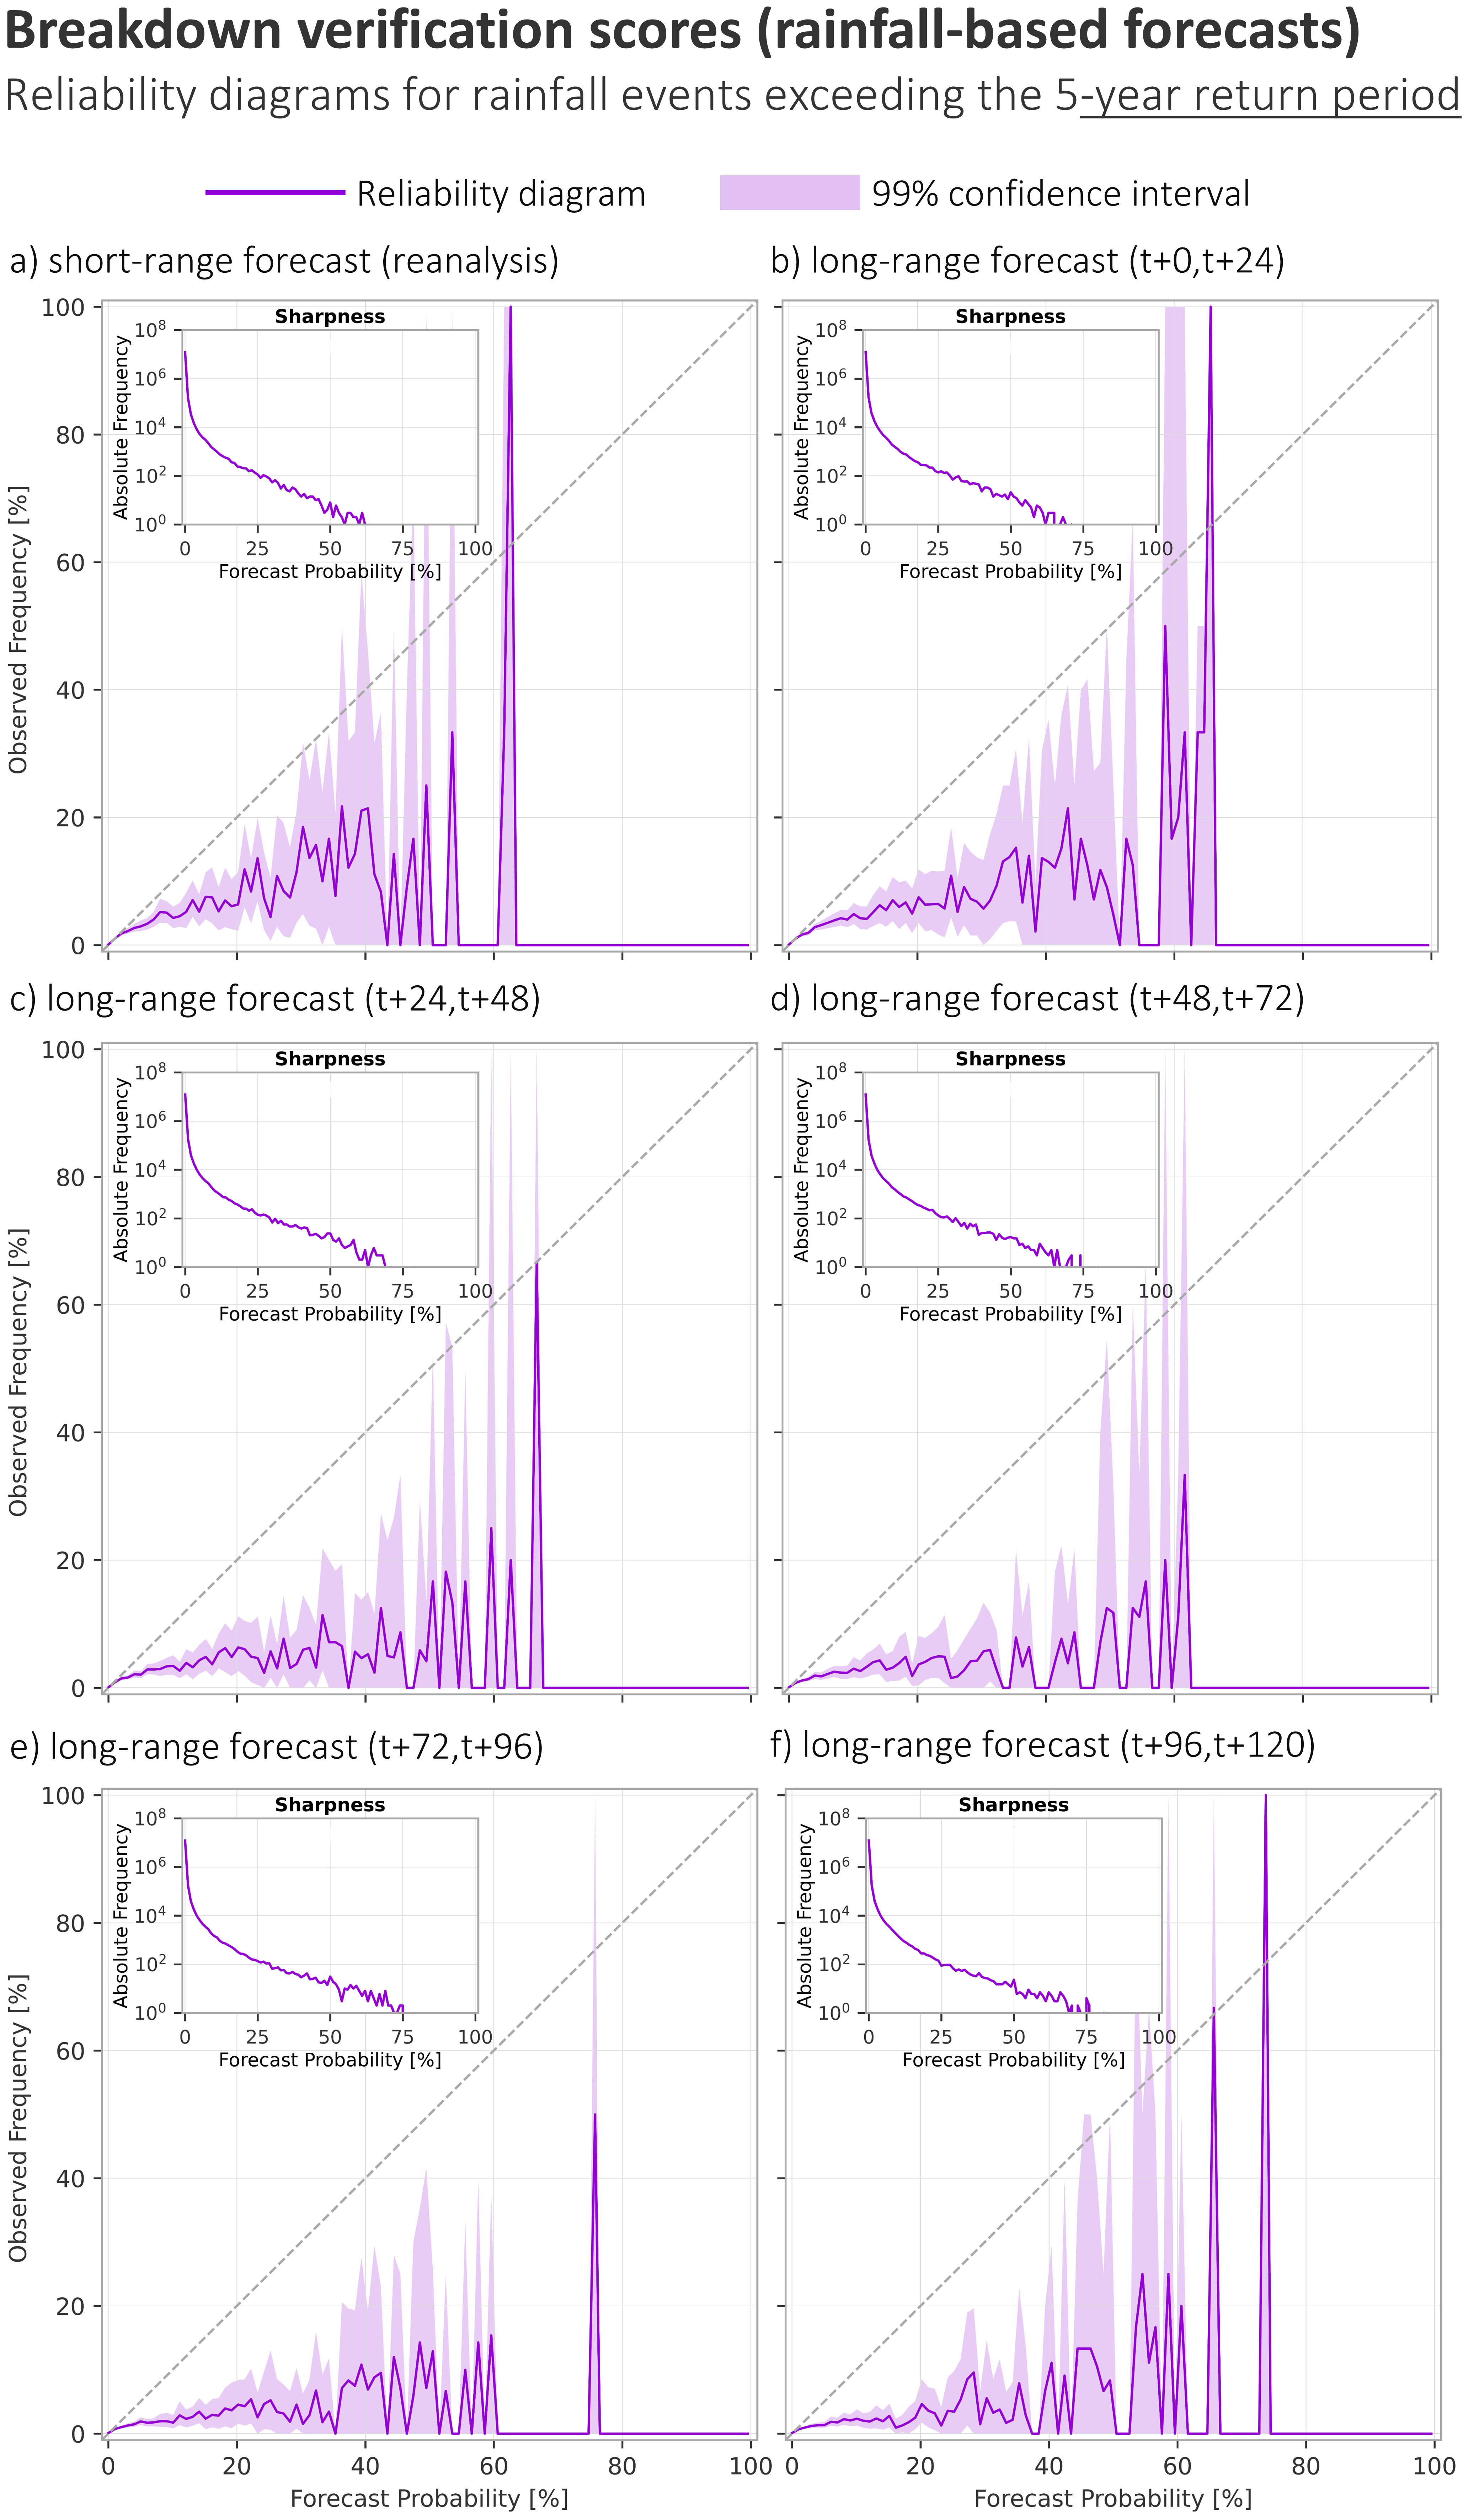
\includegraphics[width=\textwidth]{rainfall_based_ff_verif_breakdown_scores_rel_diag_5rp.png}
\caption{\textbf{Reliability diagrams for tp >= 5-year return period for the rainfall-based forecasts of areas at risk of flash floods built with ERA5-ecPoint.} Similar to Figure \ref{fig:rainfall_based_ff_verif_breakdown_scores_rel_diag_1rp}.}
\label{fig:rainfall_based_ff_verif_breakdown_scores_rel_diag_5rp}
\end{figure}

\begin{figure}[htbp]
\centering
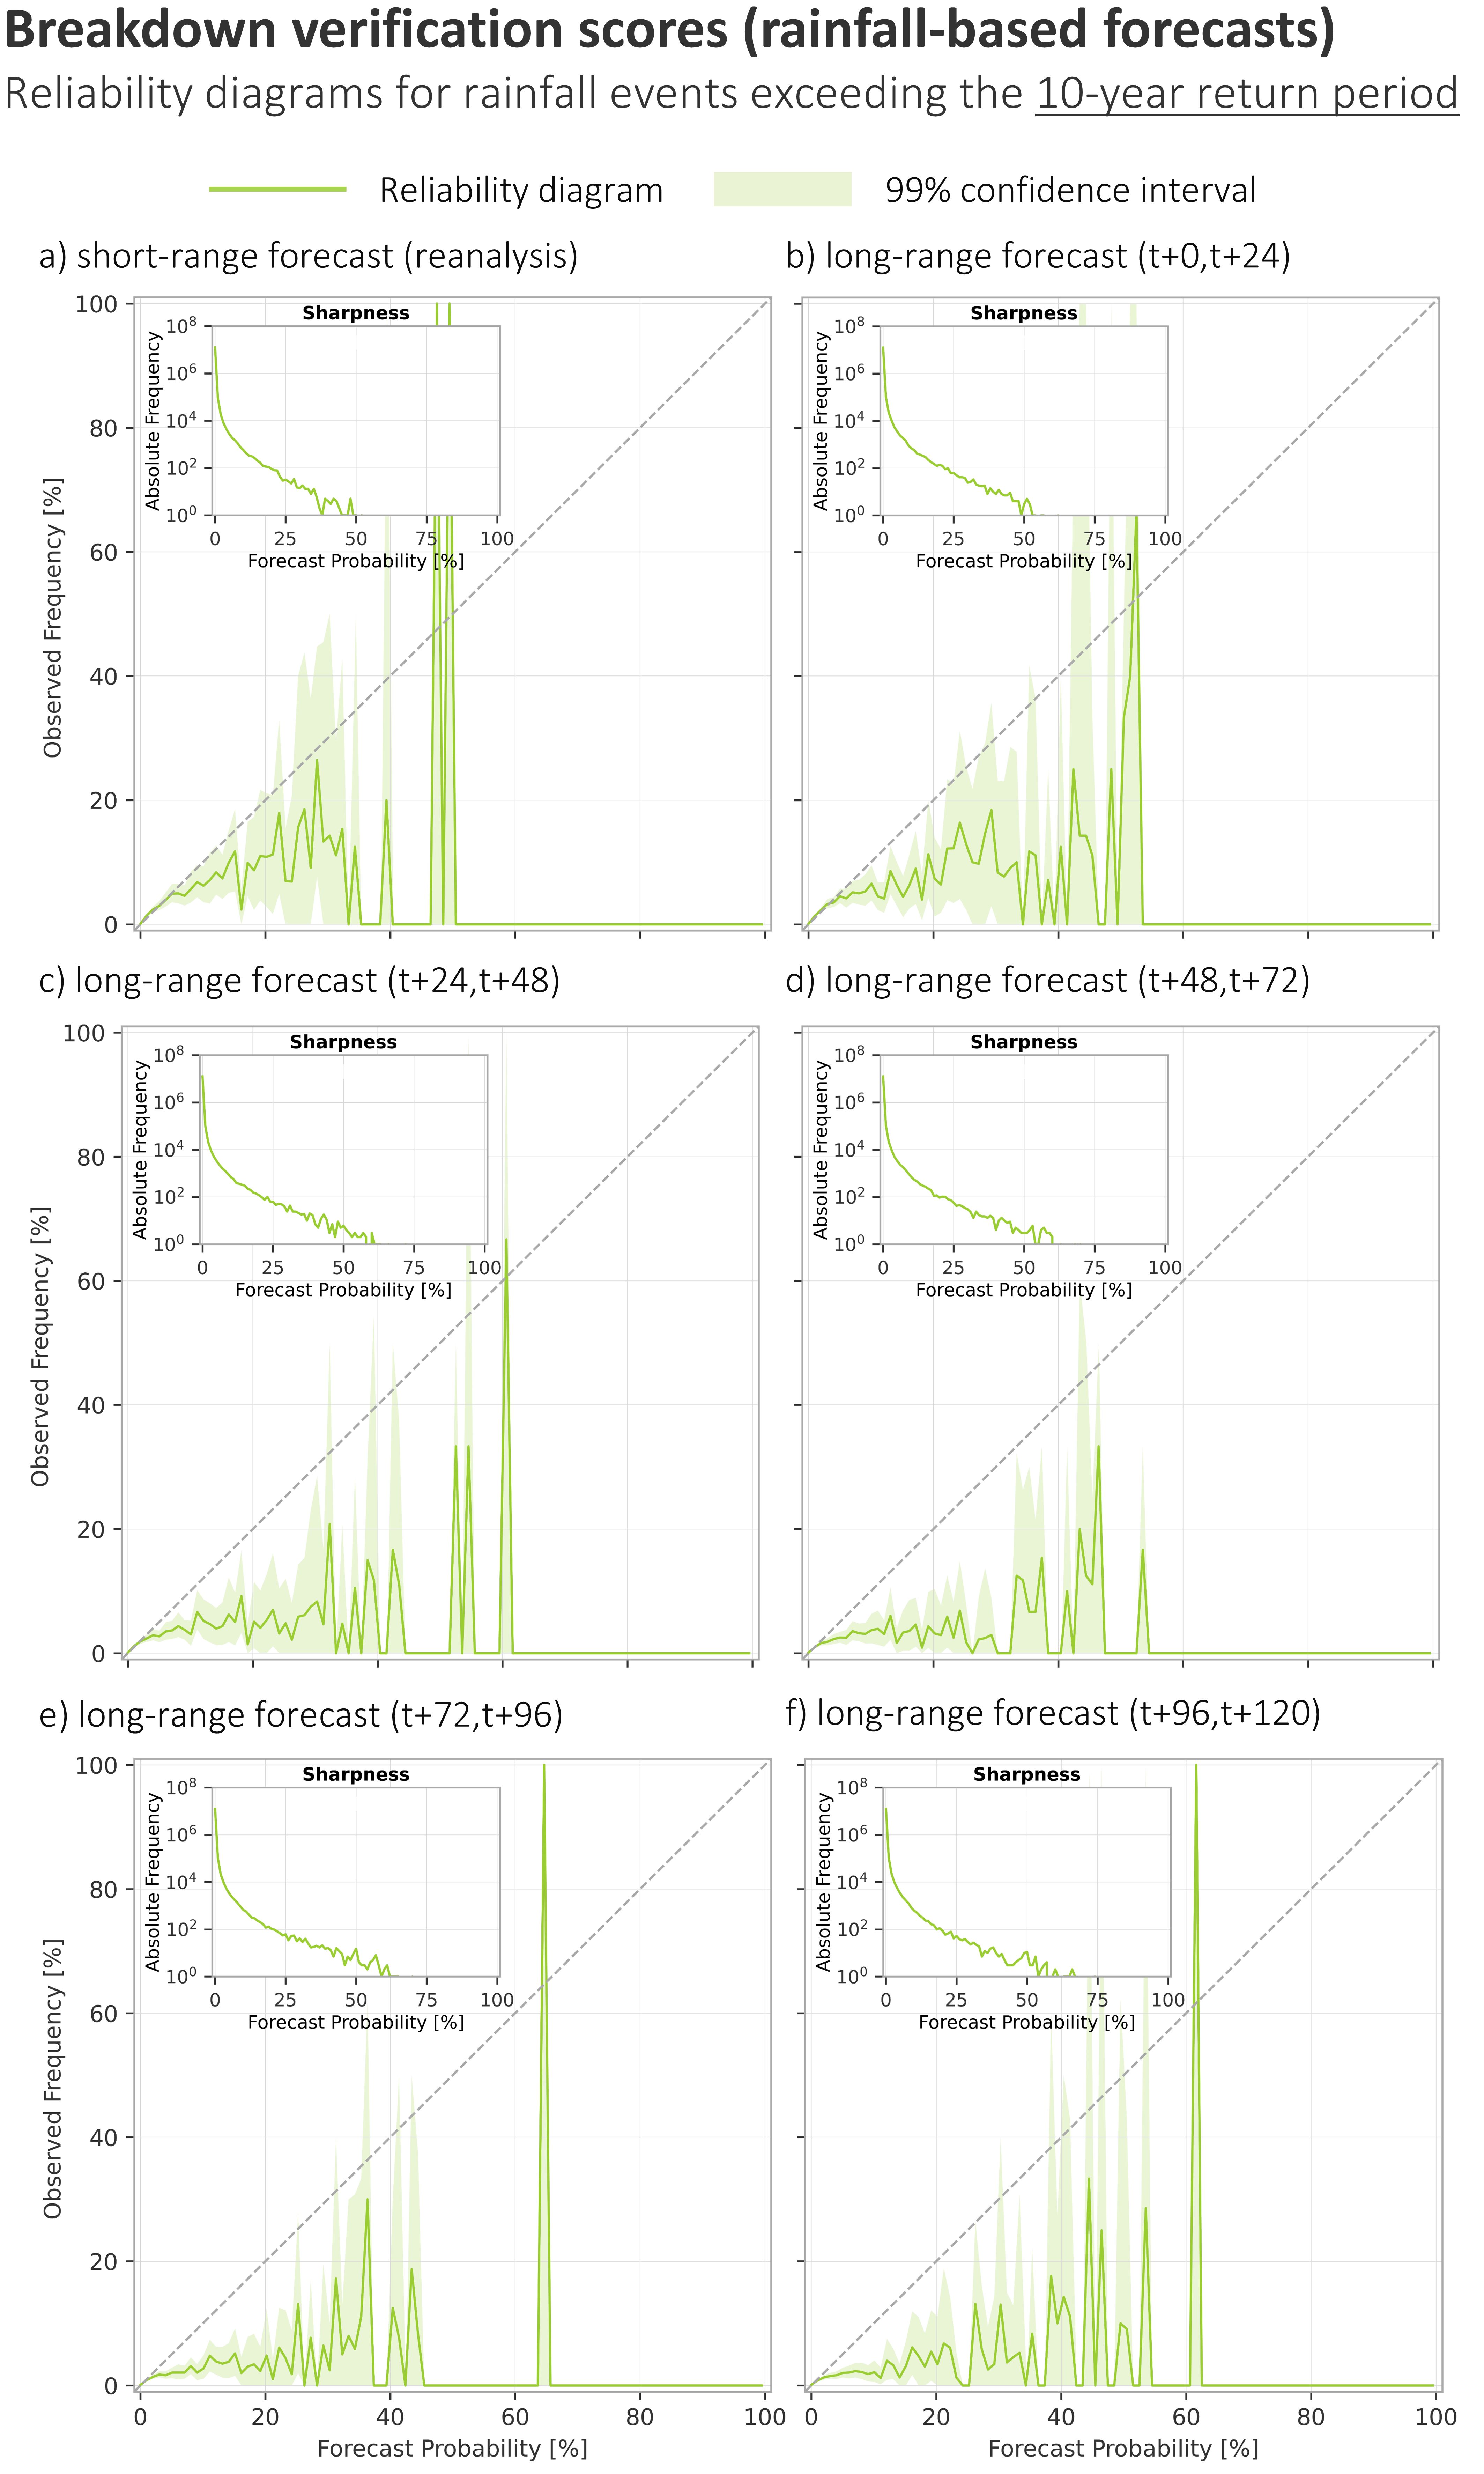
\includegraphics[width=\textwidth]{rainfall_based_ff_verif_breakdown_scores_rel_diag_10rp.png}
\caption{\textbf{Reliability diagrams for tp >= 5-year return period for the rainfall-based forecasts of areas at risk of flash floods built with ERA5-ecPoint.} Similar to Figure \ref{fig:rainfall_based_ff_verif_breakdown_scores_rel_diag_1rp}.}
\label{fig:rainfall_based_ff_verif_breakdown_scores_rel_diag_10rp}
\end{figure}

\begin{figure}[htbp]
\centering
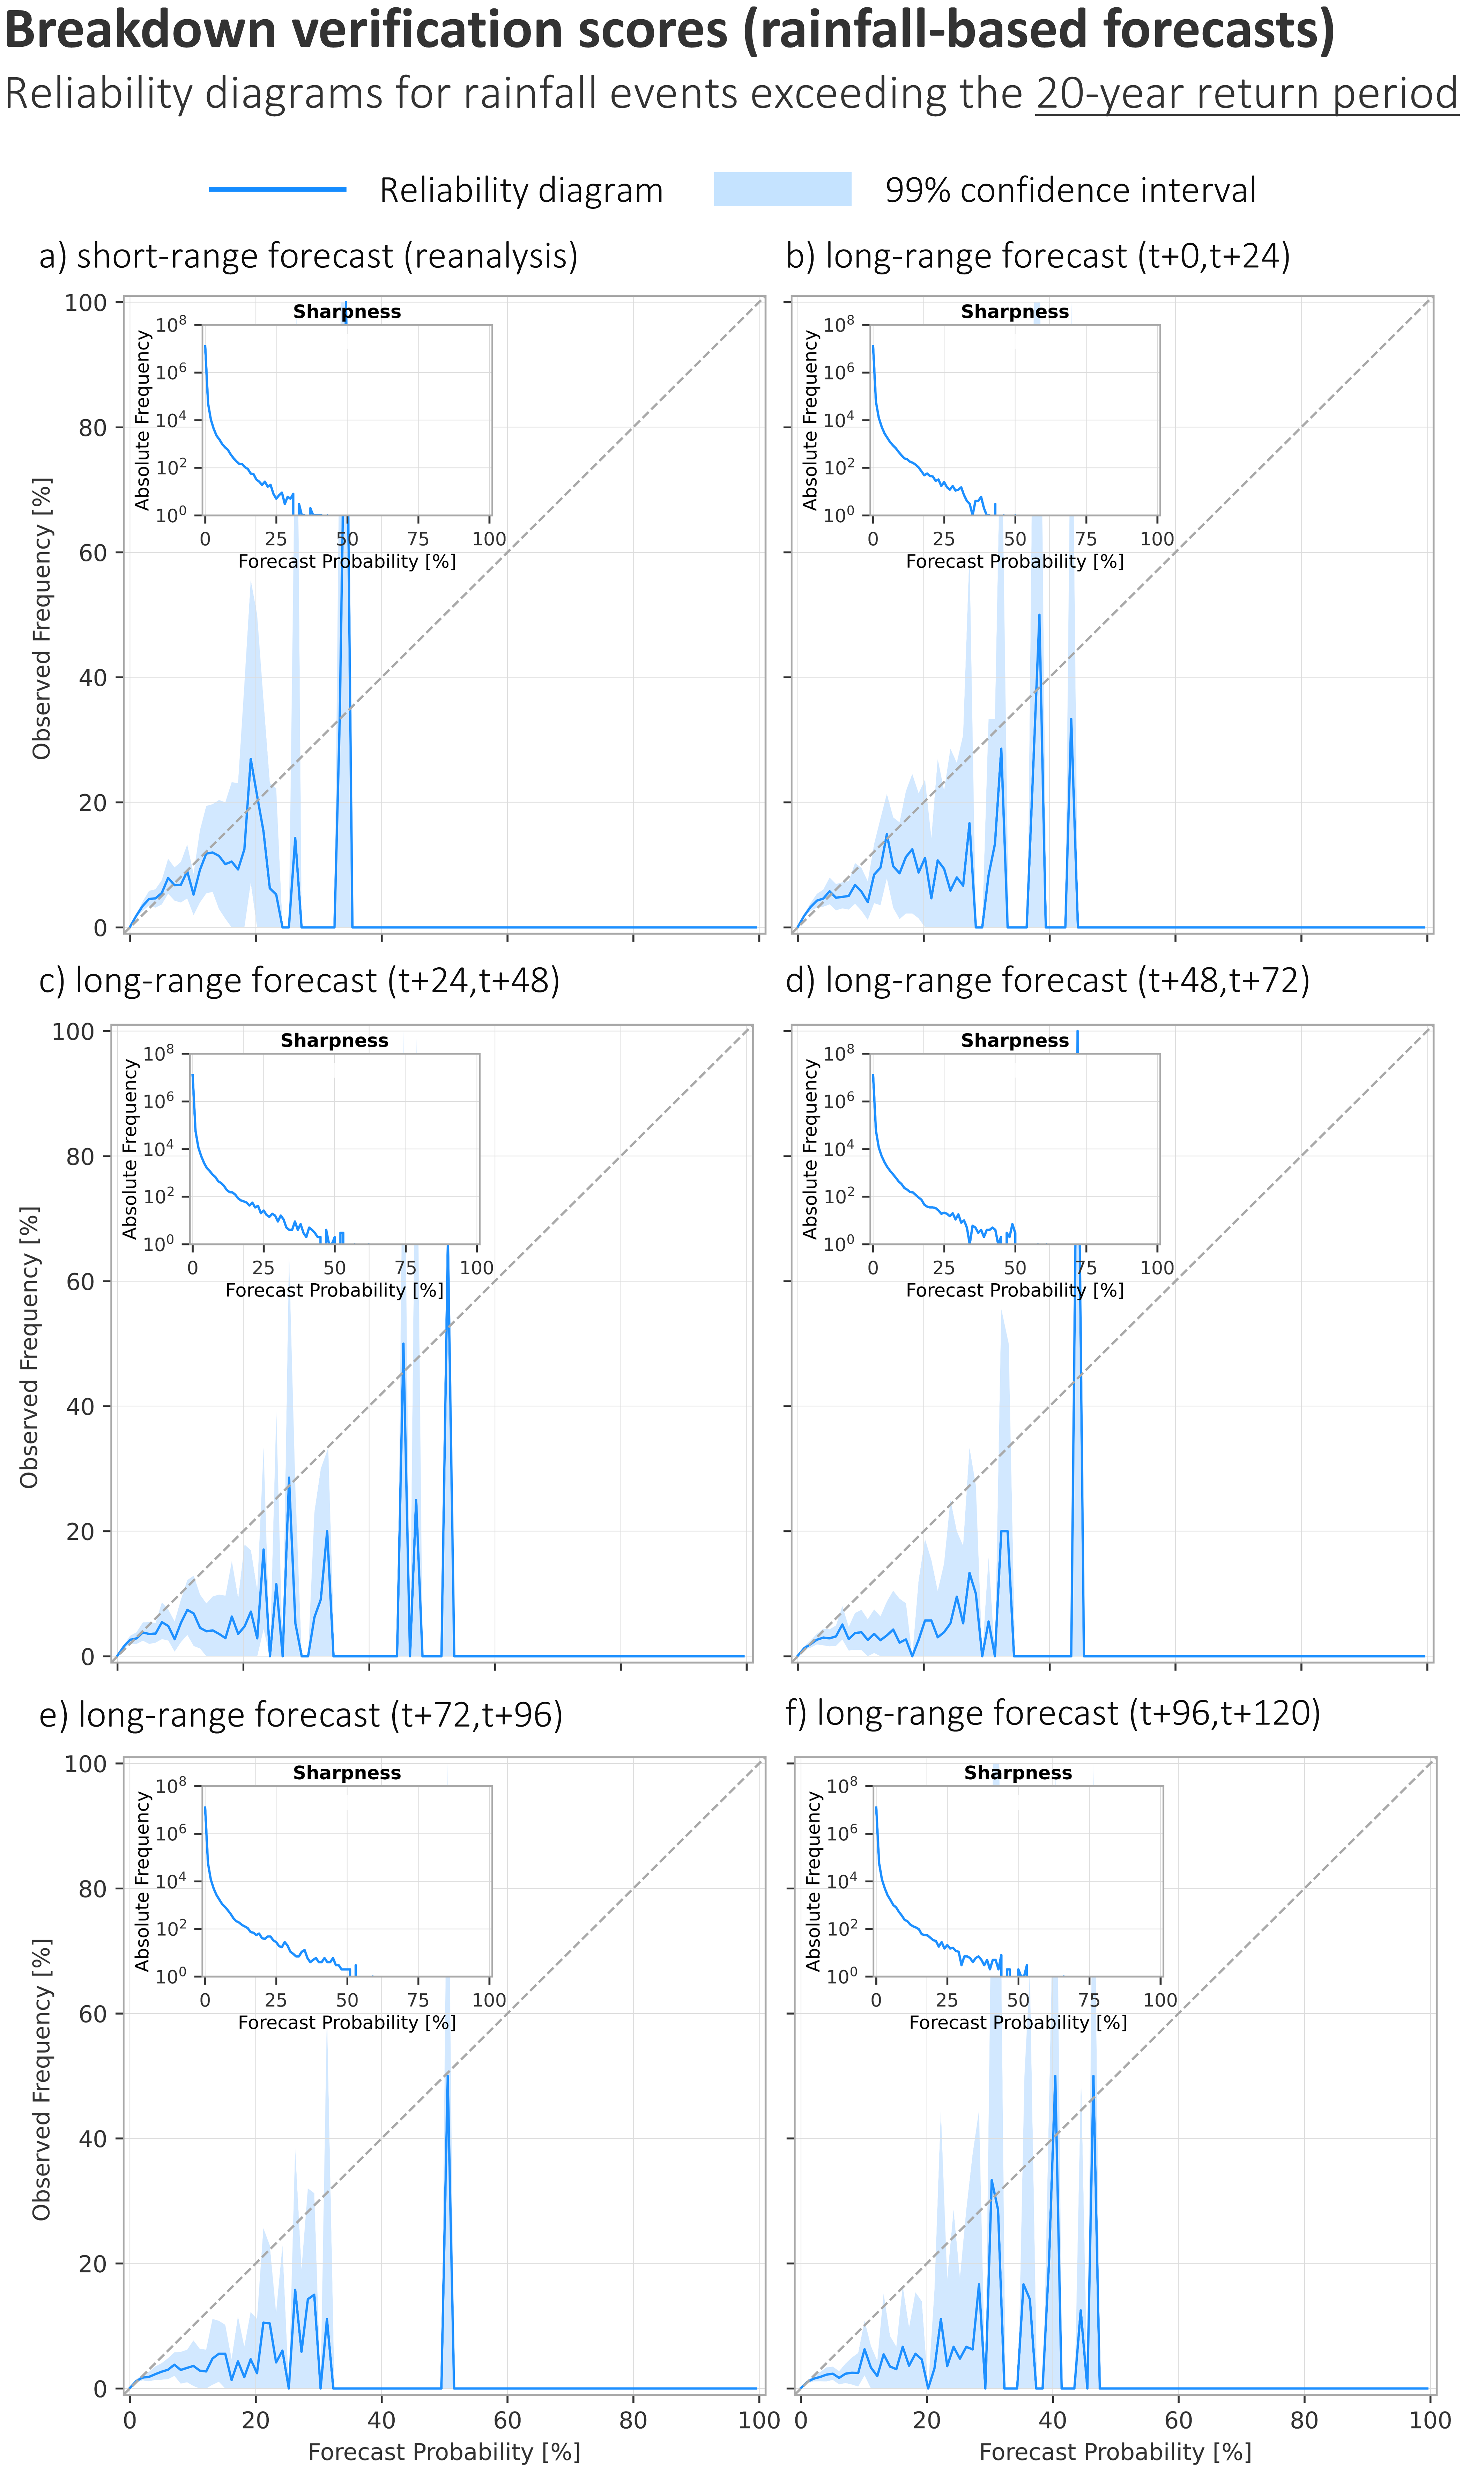
\includegraphics[width=\textwidth]{rainfall_based_ff_verif_breakdown_scores_rel_diag_20rp.png}
\caption{\textbf{Reliability diagrams for tp >= 5-year return period for the rainfall-based forecasts of areas at risk of flash floods built with ERA5-ecPoint.} Similar to Figure \ref{fig:rainfall_based_ff_verif_breakdown_scores_rel_diag_1rp}.}
\label{fig:rainfall_based_ff_verif_breakdown_scores_rel_diag_20rp}
\end{figure}

\begin{figure}[htbp]
\centering
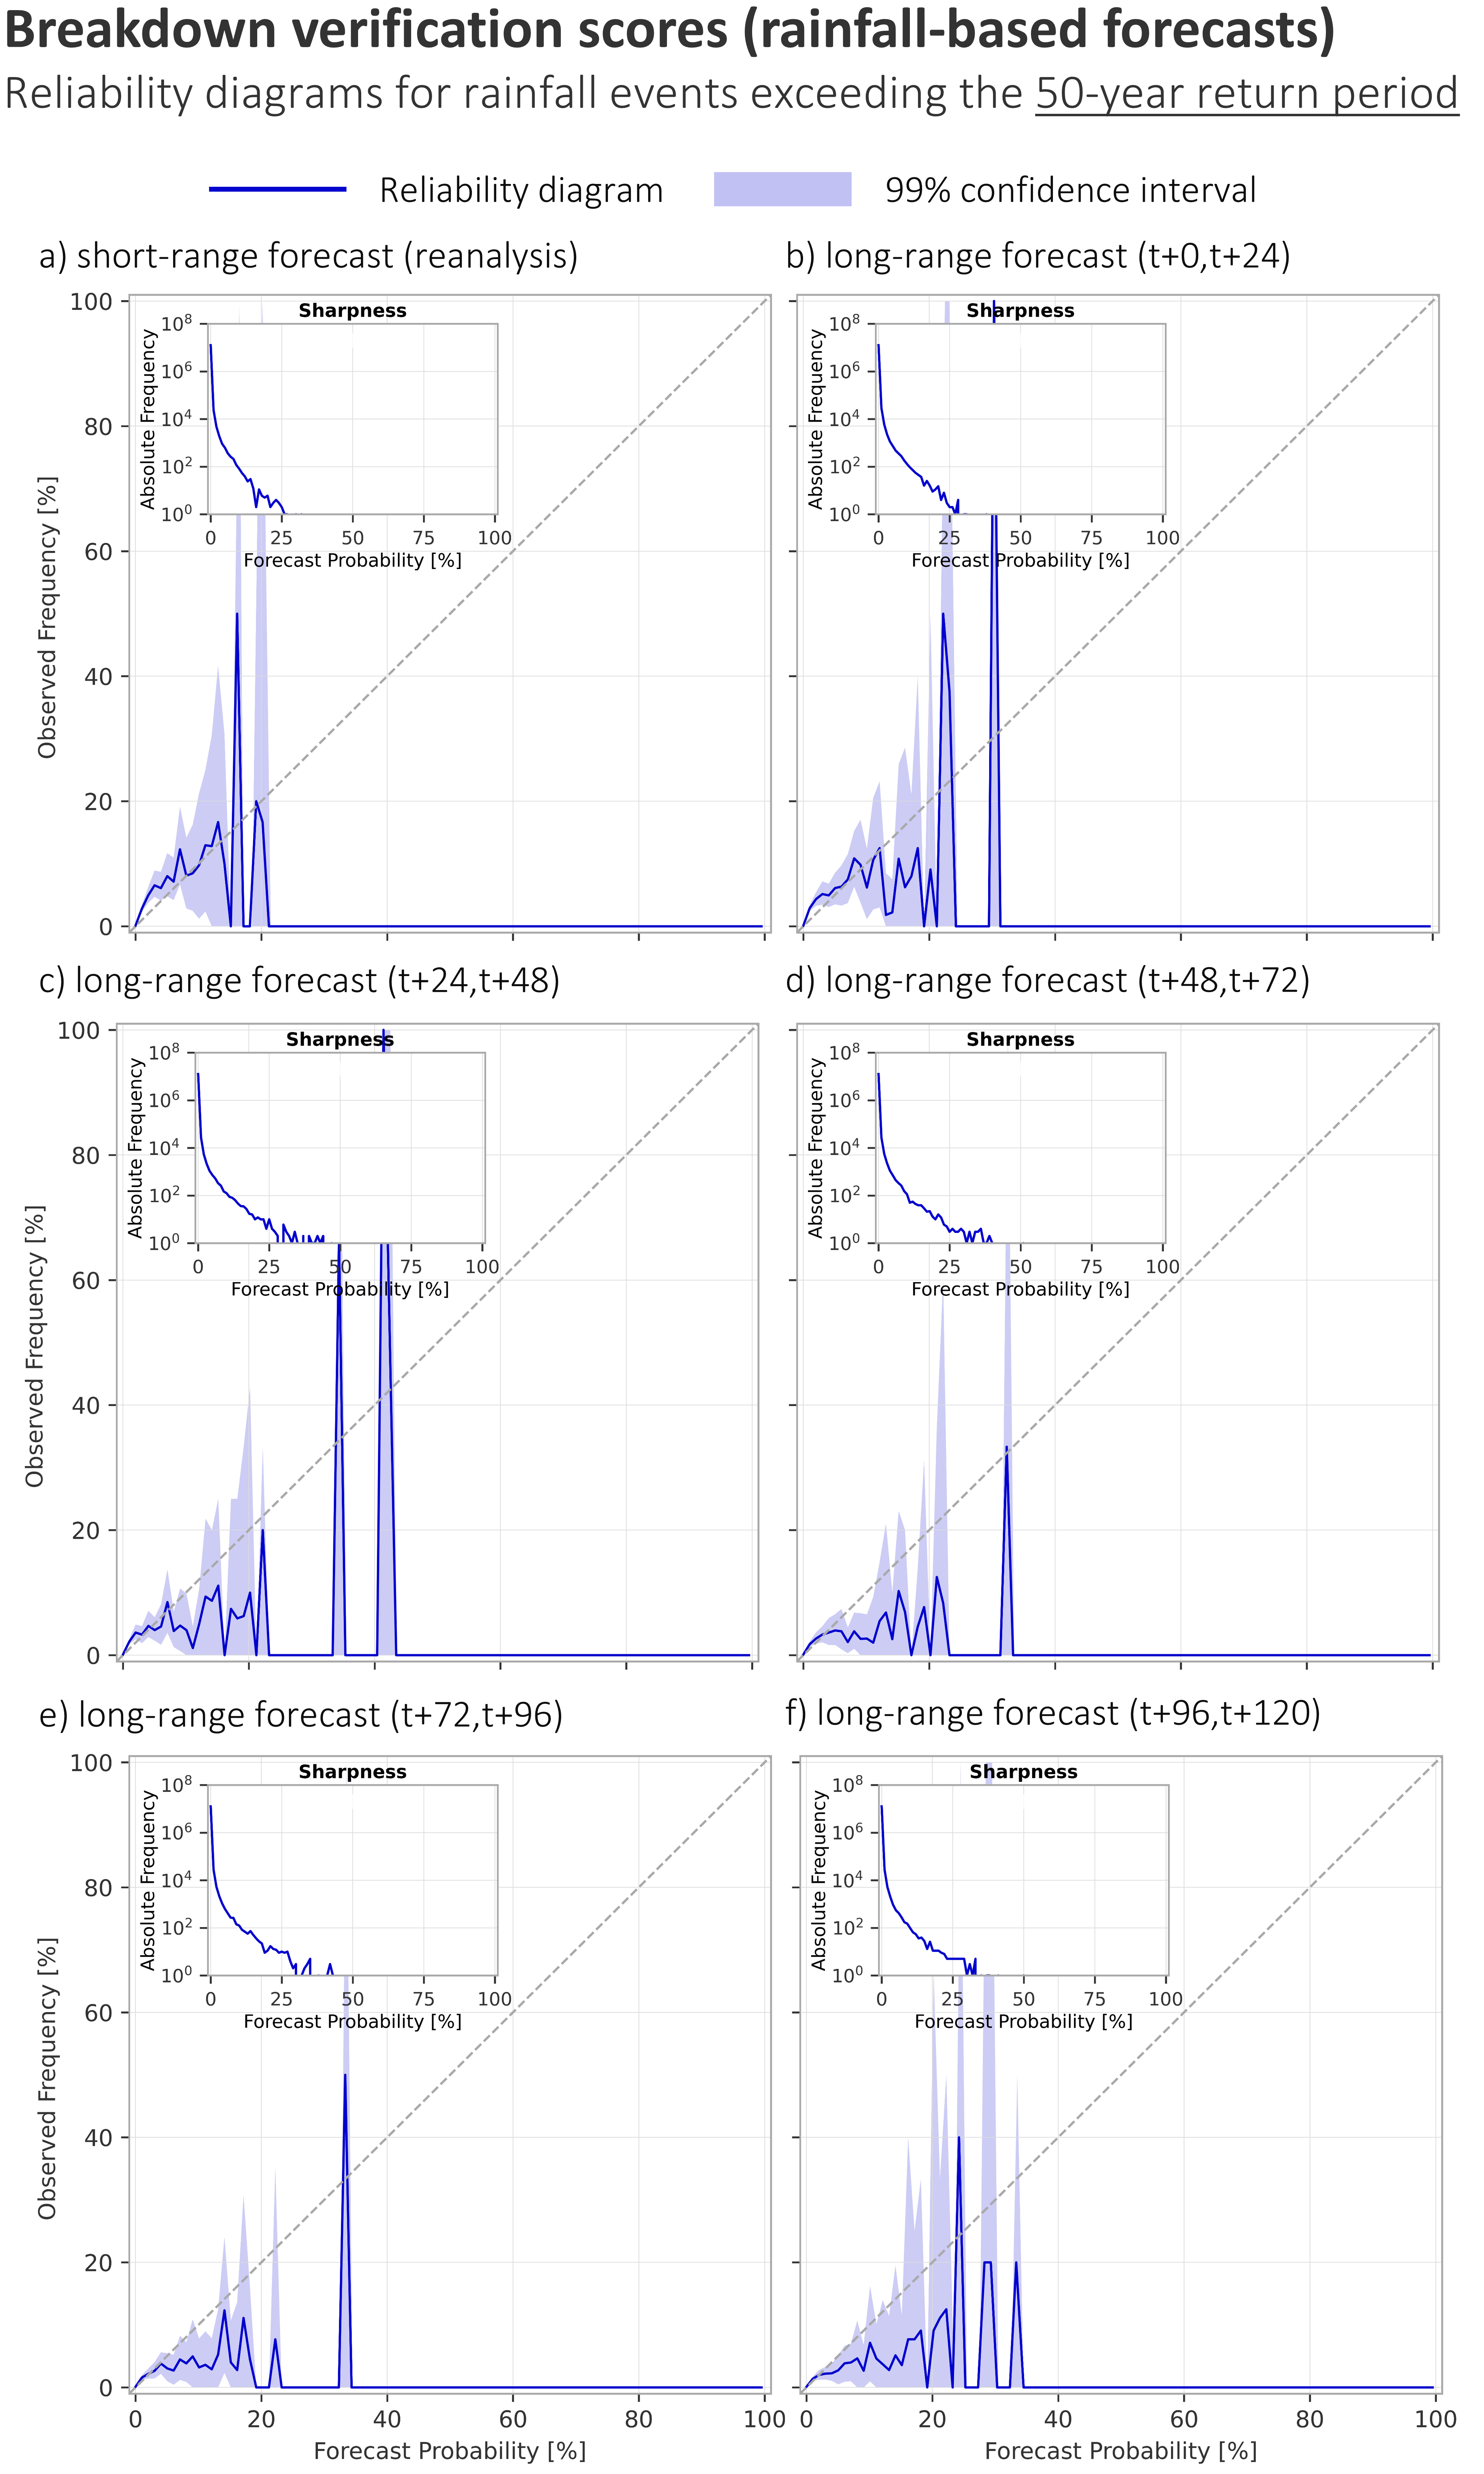
\includegraphics[width=\textwidth]{rainfall_based_ff_verif_breakdown_scores_rel_diag_50rp.png}
\caption{\textbf{Reliability diagrams for tp >= 5-year return period for the rainfall-based forecasts of areas at risk of flash floods built with ERA5-ecPoint.} Similar to Figure \ref{fig:rainfall_based_ff_verif_breakdown_scores_rel_diag_1rp}.}
\label{fig:rainfall_based_ff_verif_breakdown_scores_rel_diag_50rp}
\end{figure}

\begin{figure}[htbp]
\centering
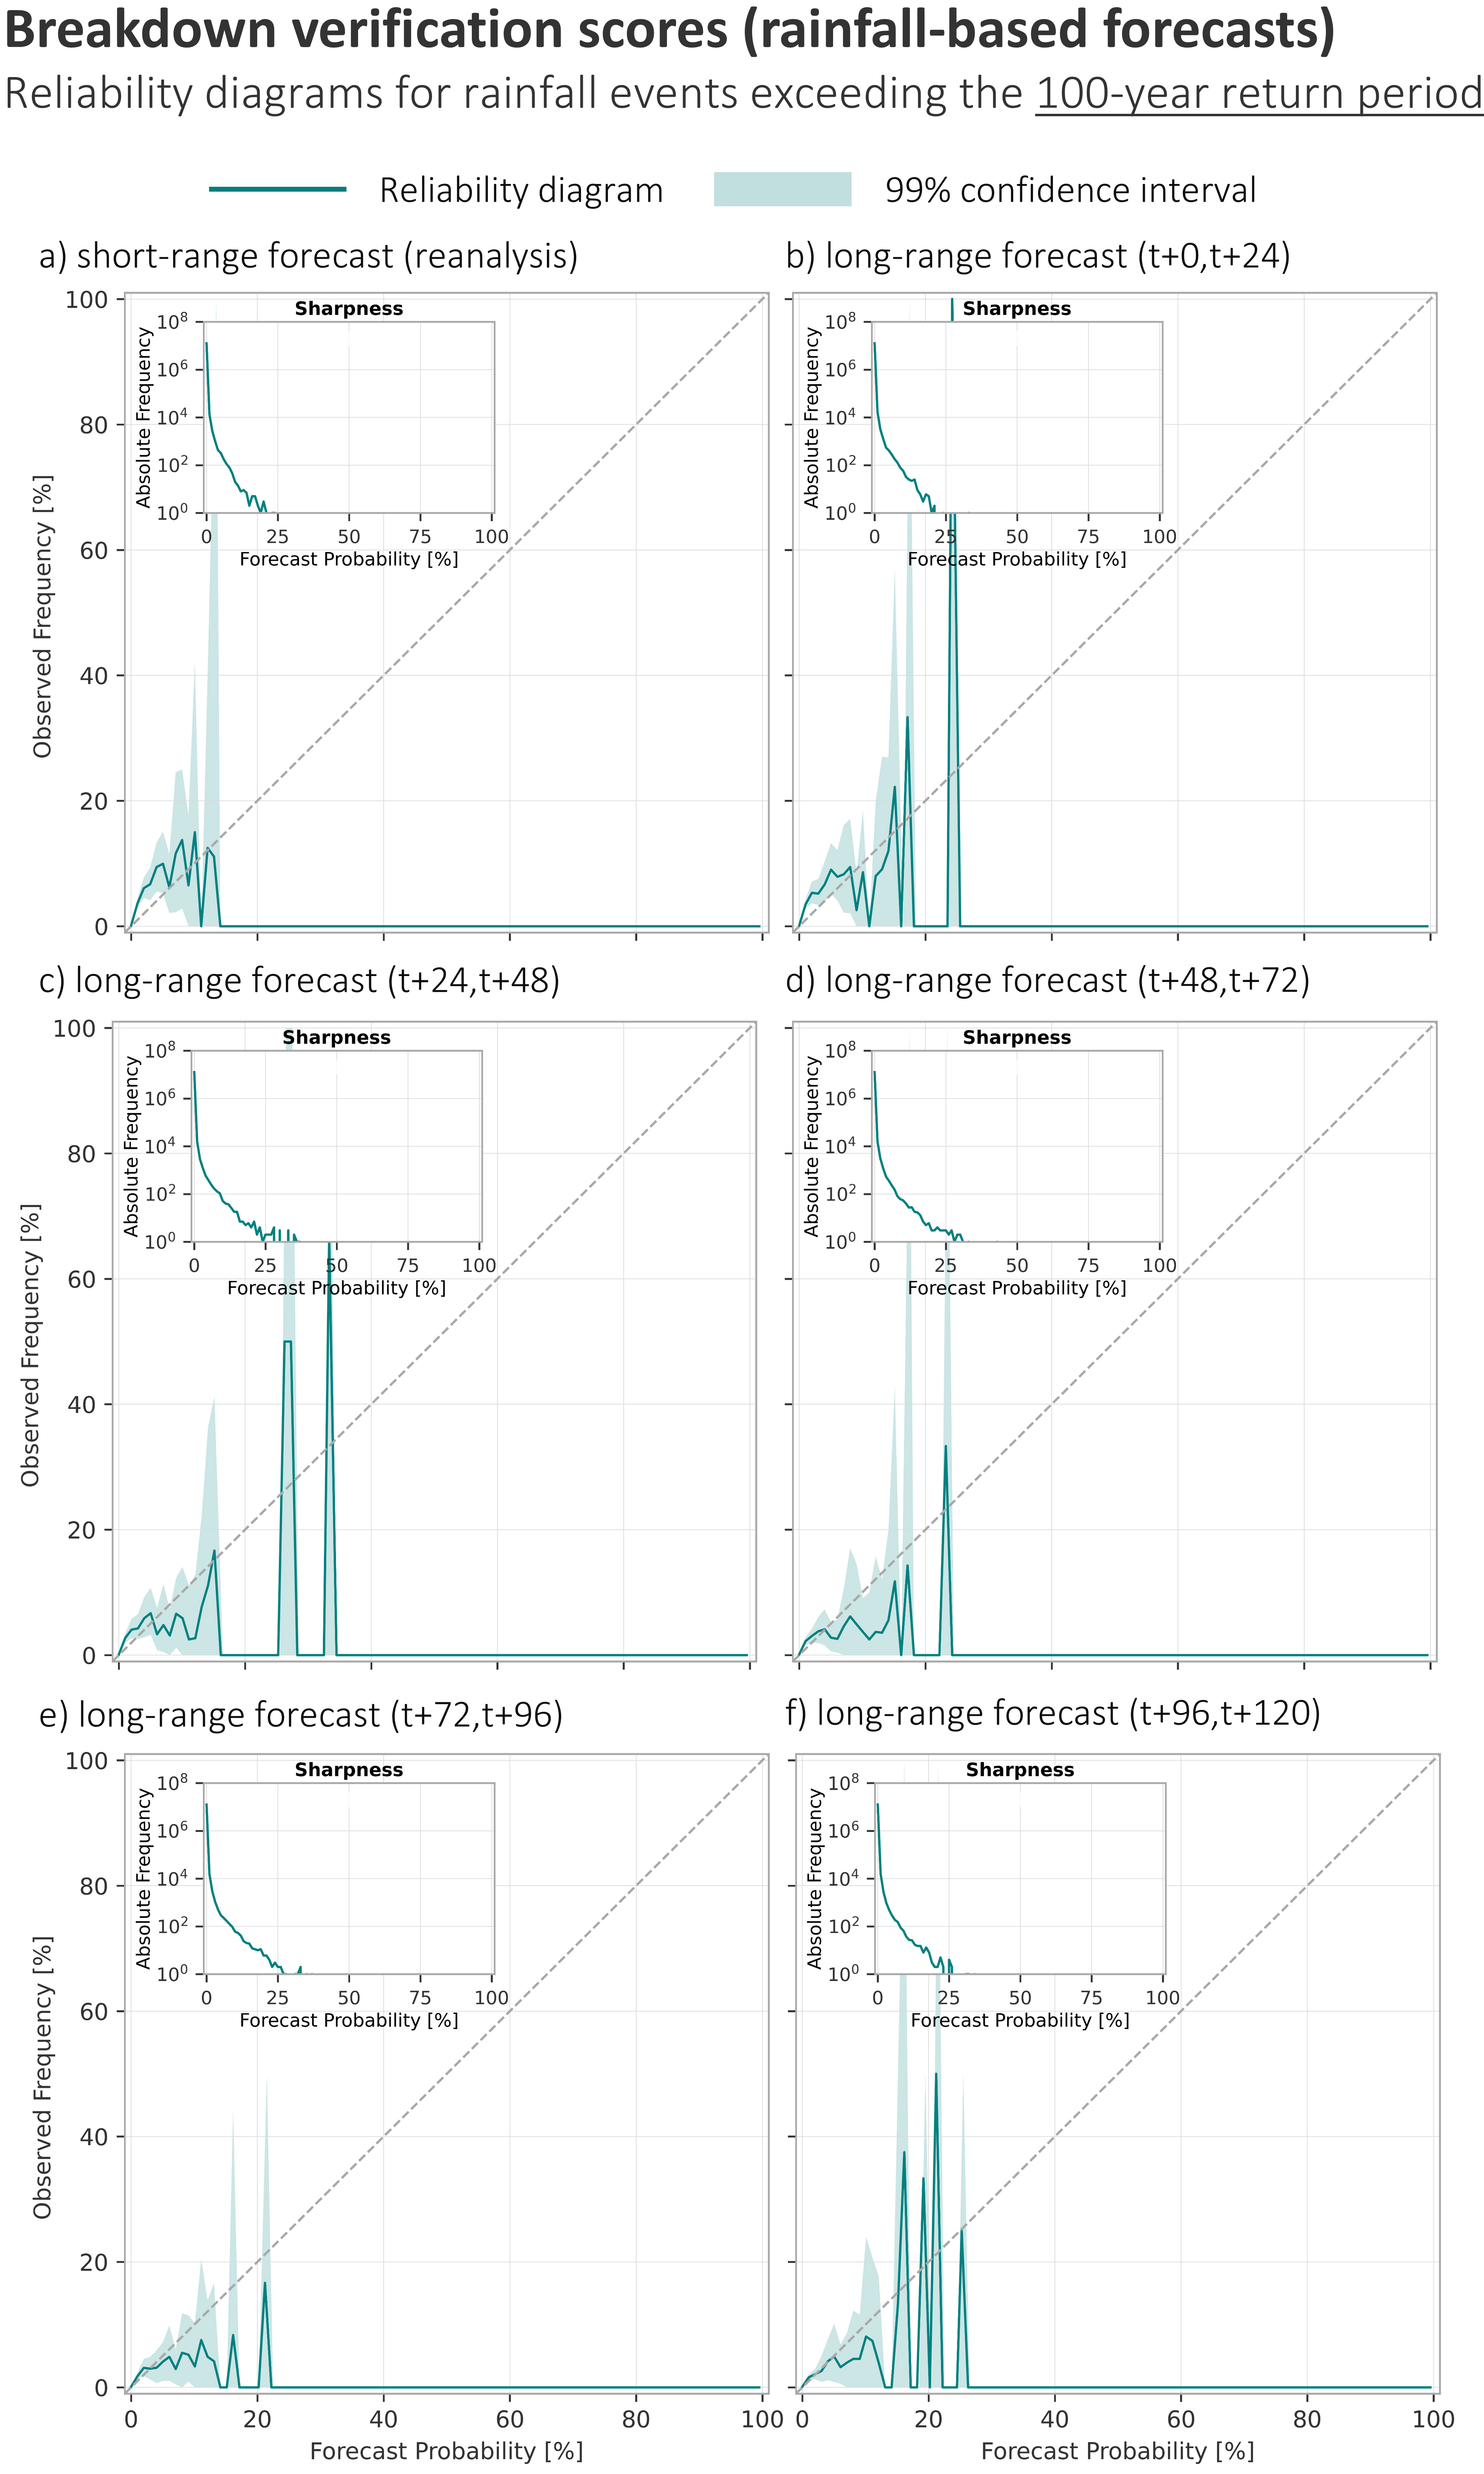
\includegraphics[width=\textwidth]{rainfall_based_ff_verif_breakdown_scores_rel_diag_100rp.png}
\caption{\textbf{Reliability diagrams for tp >= 5-year return period for the rainfall-based forecasts of areas at risk of flash floods built with ERA5-ecPoint.} Similar to Figure \ref{fig:rainfall_based_ff_verif_breakdown_scores_rel_diag_1rp}.}
\label{fig:rainfall_based_ff_verif_breakdown_scores_rel_diag_100rp}
\end{figure}

%%%%%%%%%
\section{Assessment of short-range data-driven hydro-meteorological predictions of areas at risk of flash floods}
\label{verif_data_driven_short_fc}

\subsection{Model training}

\subsubsection{Training methodology}

The development of the data-driven predictions of areas at risk of flash floods employed a systematic training approach designed to optimise predictive performance whilst ensuring generalisability due to the severe imbalance problem in the training dataset. 

The model architectures comprised decision-tree-based algorithms such as random forest and gradient boosting (XGBoost and CatBoost), and a feed-forward neural network. We considered 7 input features such as the probability of exceeding a certain rainfall return period, the maximum probability of exceeding a certain rainfall return period in the adjacent grid-boxes within a radius, the antecedent soil moisture, the steepness of the orography, and the vegetation coverage. 

The training dataset comprises 53,245 yes-events over 19,746,990 grid-boxes (0.27\% of yes-events), spanning the years between 2001 to 2020. 

To ensure a robust model evaluation and prevent overfitting, a nested cross-validation strategy was implemented, employing 5-fold cross-validation for the outer loop and 3-fold for hyperparameter optimisation in the inner loop. 

The input feature set underwent normalisation for the neural network, calculated independently for each training fold to prevent data leakage.

No missing values strategies was applied to the dataset as there not were any by design.


\subsubsection{Hyperparameter optimisation}

Hyperparameter selection employed Optuna (version 4.3.0), a state-of-the-art hyperparameter optimisation framework utilising Tree-structured Parzen Estimator (TPE) sampling. This Bayesian optimisation approach was integrated within the inner loop of the nested k-fold cross-validation procedure, ensuring unbiased performance estimates whilst identifying optimal hyperparameter configurations.

For each outer fold, an independent Optuna study was initiated with 20 trials, allowing the algorithm to explore the hyperparameter space. The objective function maximised the mean AROC across the inner k-fold cross-validation splits, with early pruning implemented via Optuna's MedianPruner to terminate unpromising trials and reduce computational overhead.

Figure \ref{fig:optuna_optimasation_convergence} illustrates the optimisation history for the five outer folds, demonstrating the TPE algorithm's efficiency in identifying high-performing configurations from the first iteration. The solid coloured lines track the trails with the "best value" for the objective (i.e. maximising AROC). The best trial appears to be in all cases trial n. 0, until convergence towards optimal values typically occurred within 10 and 15 trials. Optuna run the full set of 20 trials for all outer loops as shown in Figure \ref{fig:optuna_optimasation_convergence}.

\begin{figure}[htbp]
\centering
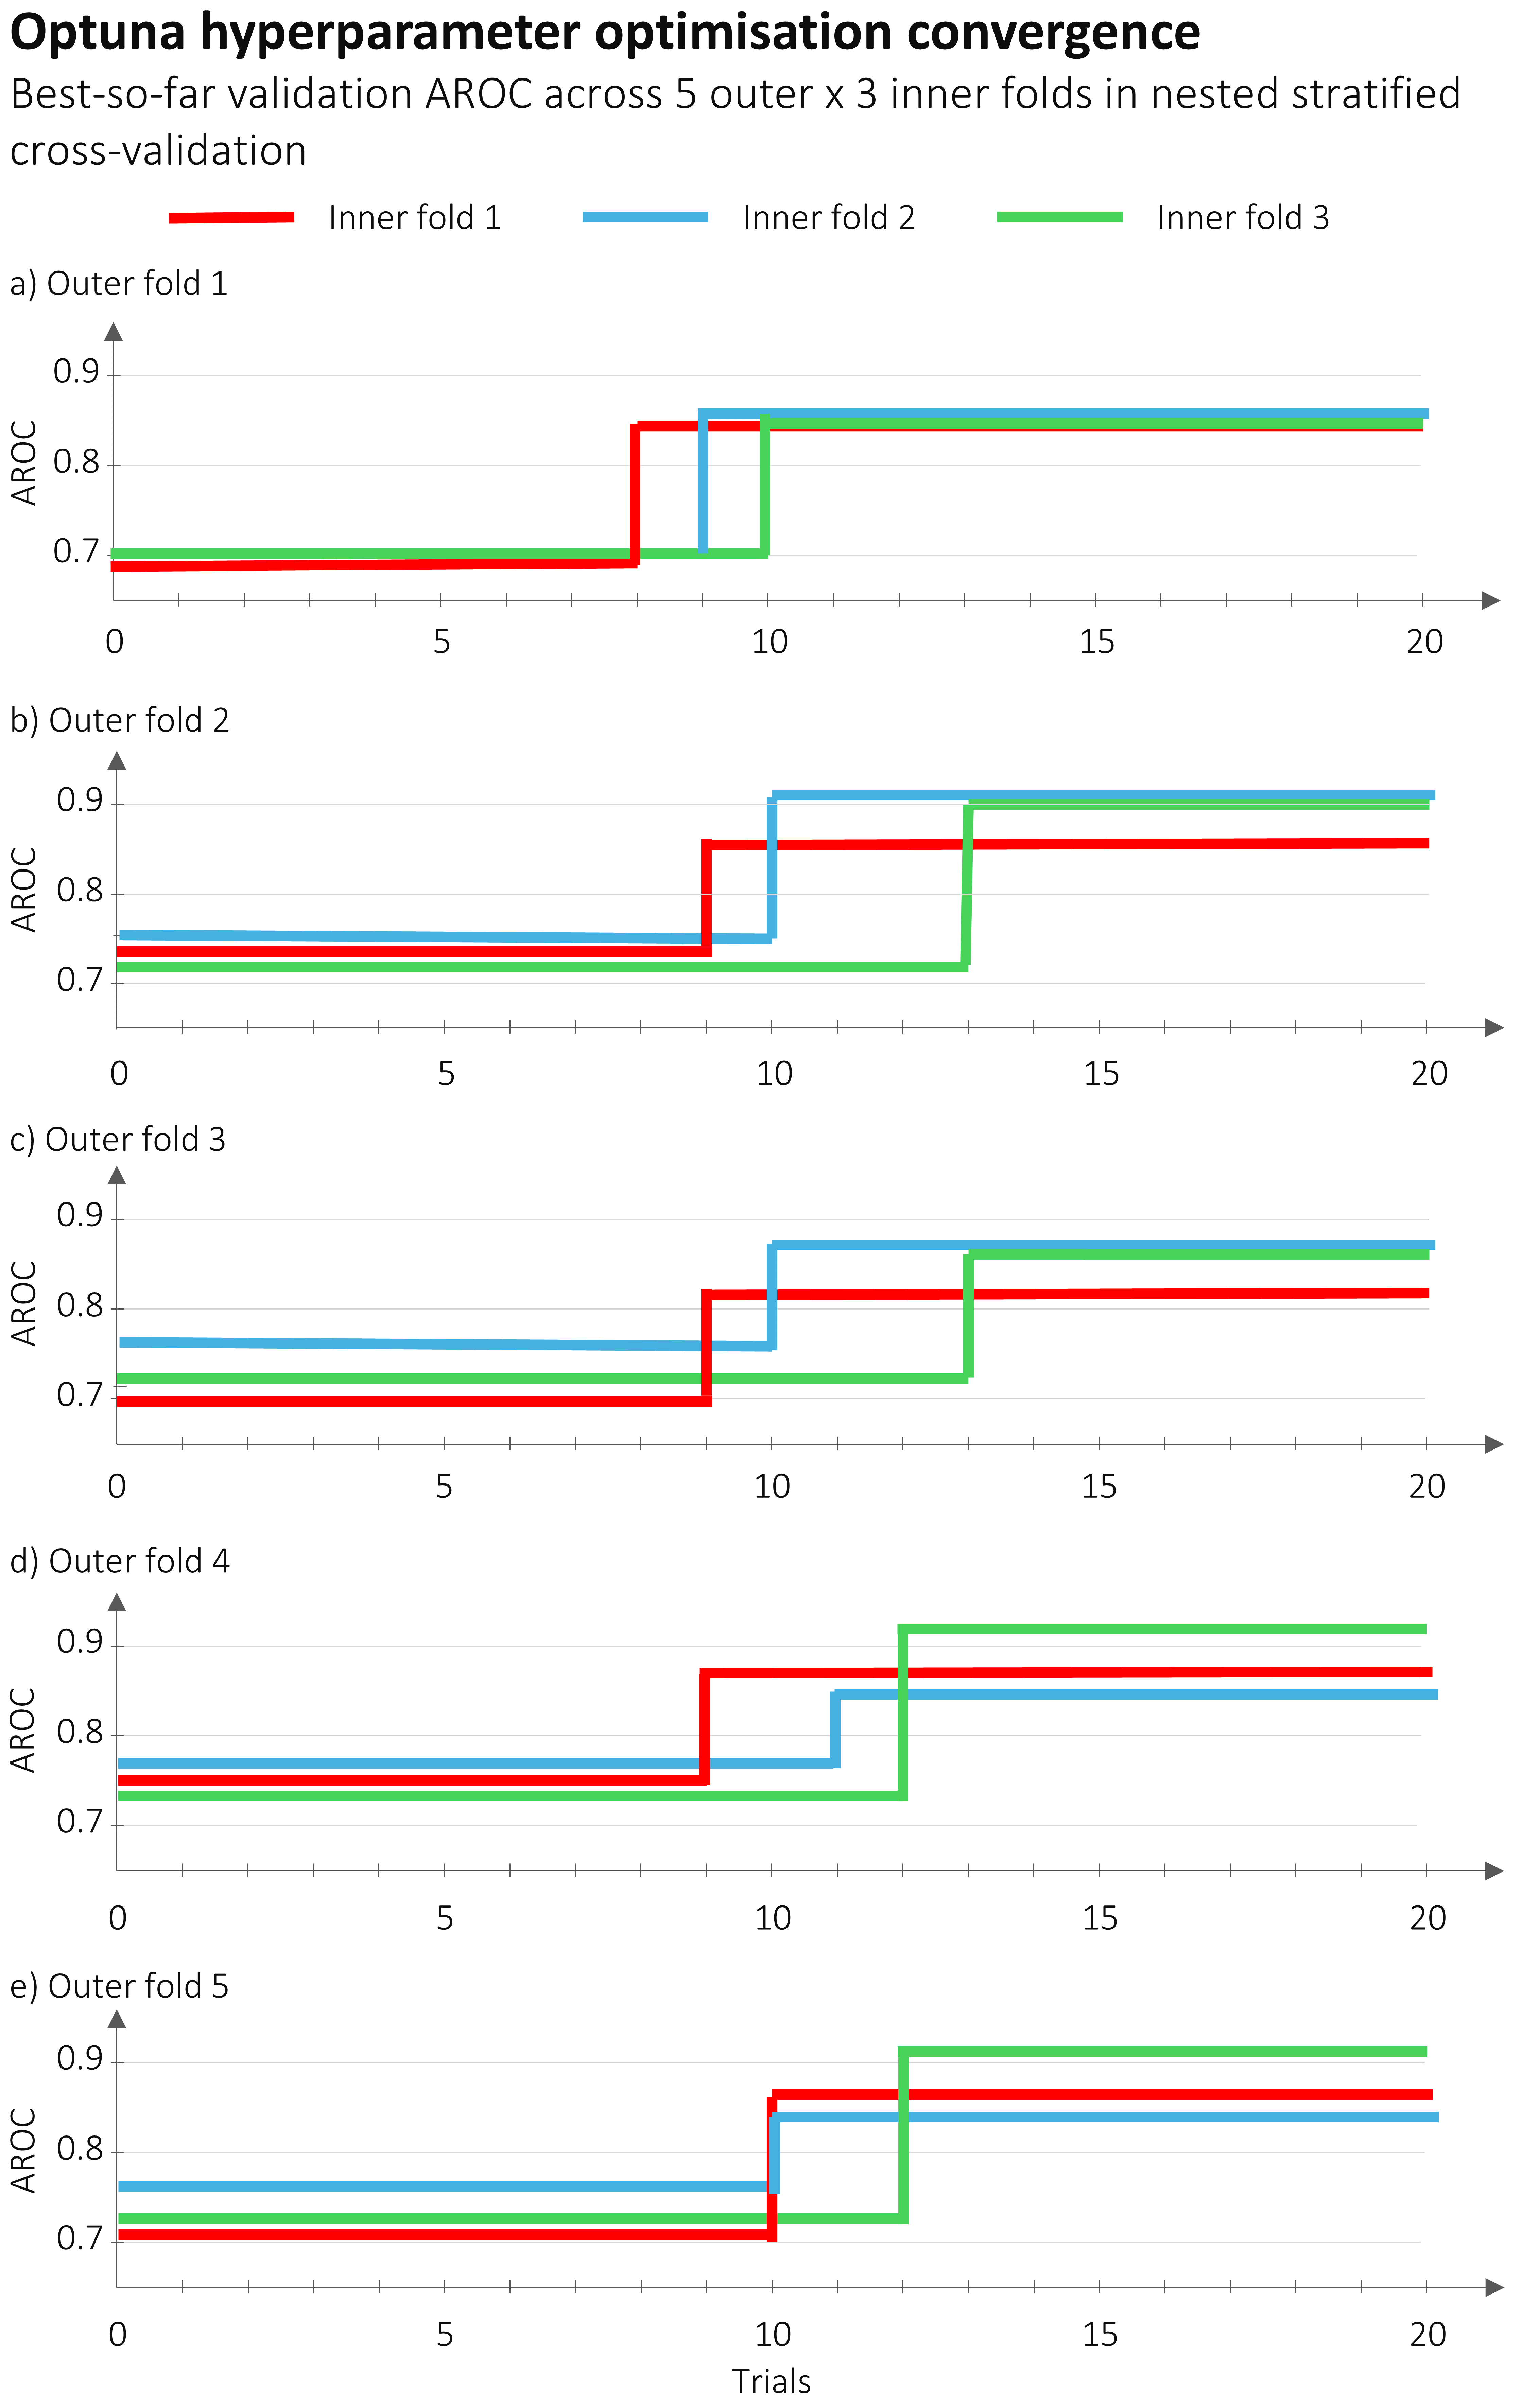
\includegraphics[width=\textwidth]{optuna_optimasation_convergence.png}
\caption{\textbf{Convergence of Optuna hyperparameter optimisation during nested stratified 5 × 3 cross-validation} Panels (a) to (e) correspond to the outer folds. Within each panel, the three coloured staircase lines show the running best validation area under ROC curve returned from the three inner folds over the 20 trials of the hyper-parameter search. A sharp improvement is typically found between trials \sim8–13, after which the curves flatten, indicating that the optimiser converges.}
\label{fig:optuna_optimasation_convergence}
\end{figure}

The optimisation procedure yielded distinct optimal configurations for each outer fold, reflecting data heterogeneity across splits. Table 4.1 summarises the selected hyperparameter values and corresponding validation performance for each fold, demonstrating reasonable consistency in optimal values despite fold-specific variations.


\subsubsection{Training progression and convergence}

Figure \ref{fig:hydro_based_ff_cross_validation_optuna_overall_scores} presents the performance stability across the five outer folds for all evaluated models for overall scores such as AROC, recall and F1-score. In all models, the AROC values exhibited remarkable consistency across folds, with the gradient boosting implementations (XGBoost and LightGBM) maintaining values between 0.84 and 0.86 throughout. The random forest variants demonstrated slightly lower (AROC between 0.81 and 0.83) but equally stable performance. The CatBoost implementation of gradient boosting showed the lowest performance (AROC \sim0.8) of all decision-tree-based models, and the feed-forward neural network showed the lowest performance with AROC values between 0.78 and 0.8. While XGBoost remains the best model based on the recall and the F1-score, the model ranking based on these metrics shows higher variability depending on the outer fold. The small variations in the scores' absolute values suggest that such ranking differences are primarily attributable to class imbalance sensitivity to rare positive instances rather than training instability. 

\begin{figure}[htbp]
\centering
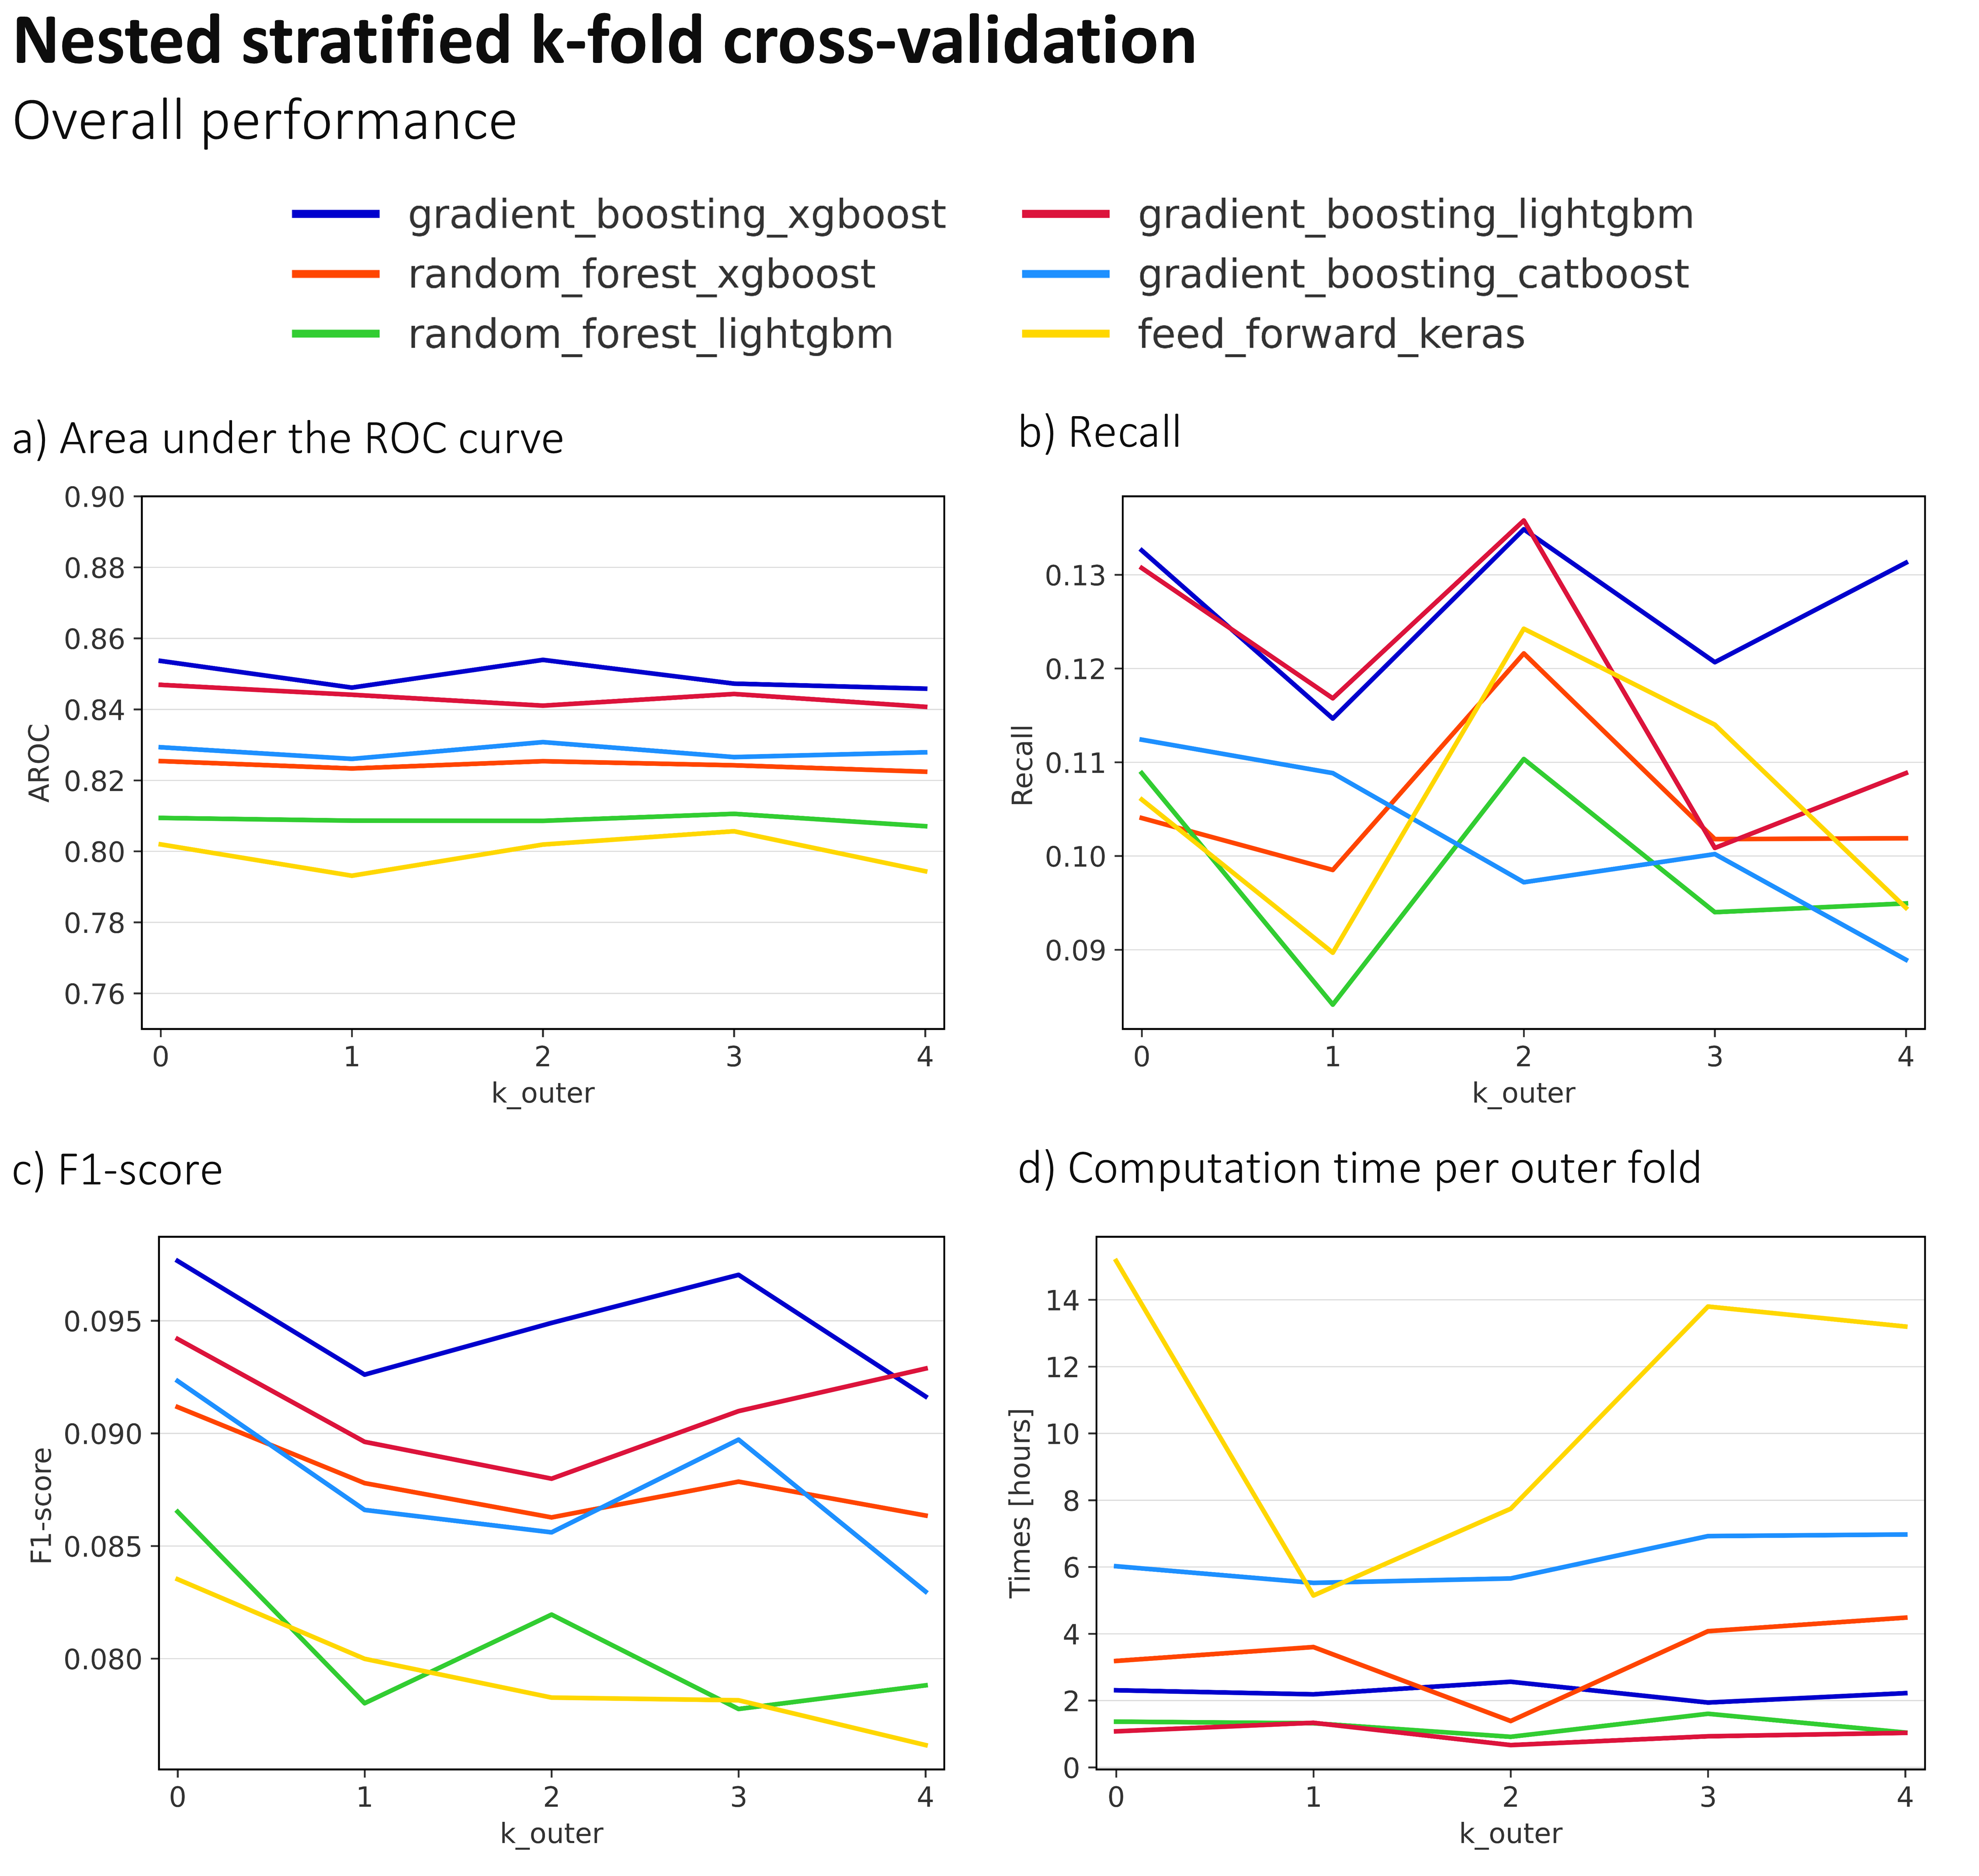
\includegraphics[width=\textwidth]{hydro_based_ff_cross_validation_optuna_overall_scores.png}
\caption{\textbf{Overall scores to estimate the model performance during the nested stratified k-fold cross validation.} Panels (a) to (d) show the values for, respectively, the area under the ROC curve, recall, F1-score, and training + hyperparameter optimisation time per outer fold. The solid colour lines represent the different models: gradient boosting - XGBoost implementation - in blue, gradient boosting - LightGBM implementation - in red, gradient boosting - CatBoost implementation - in cyan, random forest - XGBoost implementation - in orange, random forest - LightGBM implementation - in green, and feed forward neural network in yellow.}
\label{fig:hydro_based_ff_cross_validation_optuna_overall_scores}
\end{figure}

The ROC curves and the reliability diagrams (Figure \ref{fig:hydro_based_ff_cross_validation_optuna_breakdown_scores}) further illustrate the convergence quality by examining the discrimination ability and the reliability consistency across folds. Overall, the gradient boosting models (XGBoost - first column, LightGBM - second column, and Catboost - third column) show the best ROC curves and reliability diagrams, compared to the random forest implementations and the neural network, with high consistency across the outer folds. However, XGBoost shows again the best performance of all with the "optimal operating point" in the ROC curves being at a hit rate around \sim0.8 and a false alarm rate around only \sim0.3, and predicted probabilities in the reliability diagram closely aligning with the observed frequencies across most probability ranges (up to 25\% and reaching 50\% in the outer fold 1). While the other models show similar ROC curves, although with optimal operating points around hit rate of \sim0.7 for the decision-tree-based models and \sim0.6 for the neural network, the reliability diagrams for this models show a tendency to overestimate (i.e. the diagrams lie below the diagonal) from probabilities exceeding 10\% for the LightGBM and CatBoost implementations of the gradient boosting, and for almost all probability ranges in the random forest implementation of LightGBM. The XGBoost implementation of the random forest model shows a similar reliability to the XGBoost implementation of the gradient boosting, but the discrimination ability of the latter model is superior (better ROC curves over all outer folds). This suggests that \textit{gradient boosting} performs overall better than random forests when using imbalanced training datasets.

Special attention should be given to the neural network as it shows an overall good reliability (i.e. the predicted probabilities are close to the diagonal) but,  compared to the decision-tree-based models, the neural network does not provide high predicted probabilities, as they do not exceed 25\% (it reaches 50\% in only one outer fold). This behaviour suggests that the neural network demonstrates a conservative but reliable forecasting behaviour. While the neural network restraint in issuing high-probability forecasts might reflect a better uncertainty quantification and more reliable risk communication for operational deployment, the XGBoost implementation of the gradient boosting shows that predicted probabilities higher than 25\% can also be reliable between 30\% and 50\%. This restricted probability range in the neural network predictions presents operational challenges, as the model fails to differentiate between moderate and high-risk events, as shown by the lower discrimination ability of the neural network compared to XGBoost.. The inability to forecast probabilities above 25\% effectively compresses the decision space for emergency managers, who require clearer discrimination between events warranting different levels of response. Whilst a forecast of 25\% probability might trigger initial preparedness measures, operational protocols often stipulate enhanced response actions at higher probability thresholds (e.g., 40\%, 60\%). The neural network's truncated probability distribution therefore limits its utility in supporting graduated response strategies, potentially resulting in either insufficient preparation for genuinely high-risk events or uniform treatment of situations with materially different risk levels. This operational limitation suggests that, despite its superior calibration at lower probabilities, the neural network may be less suitable than the gradient boosting approaches for applications requiring nuanced risk stratification.

\begin{figure}[htbp]
\centering
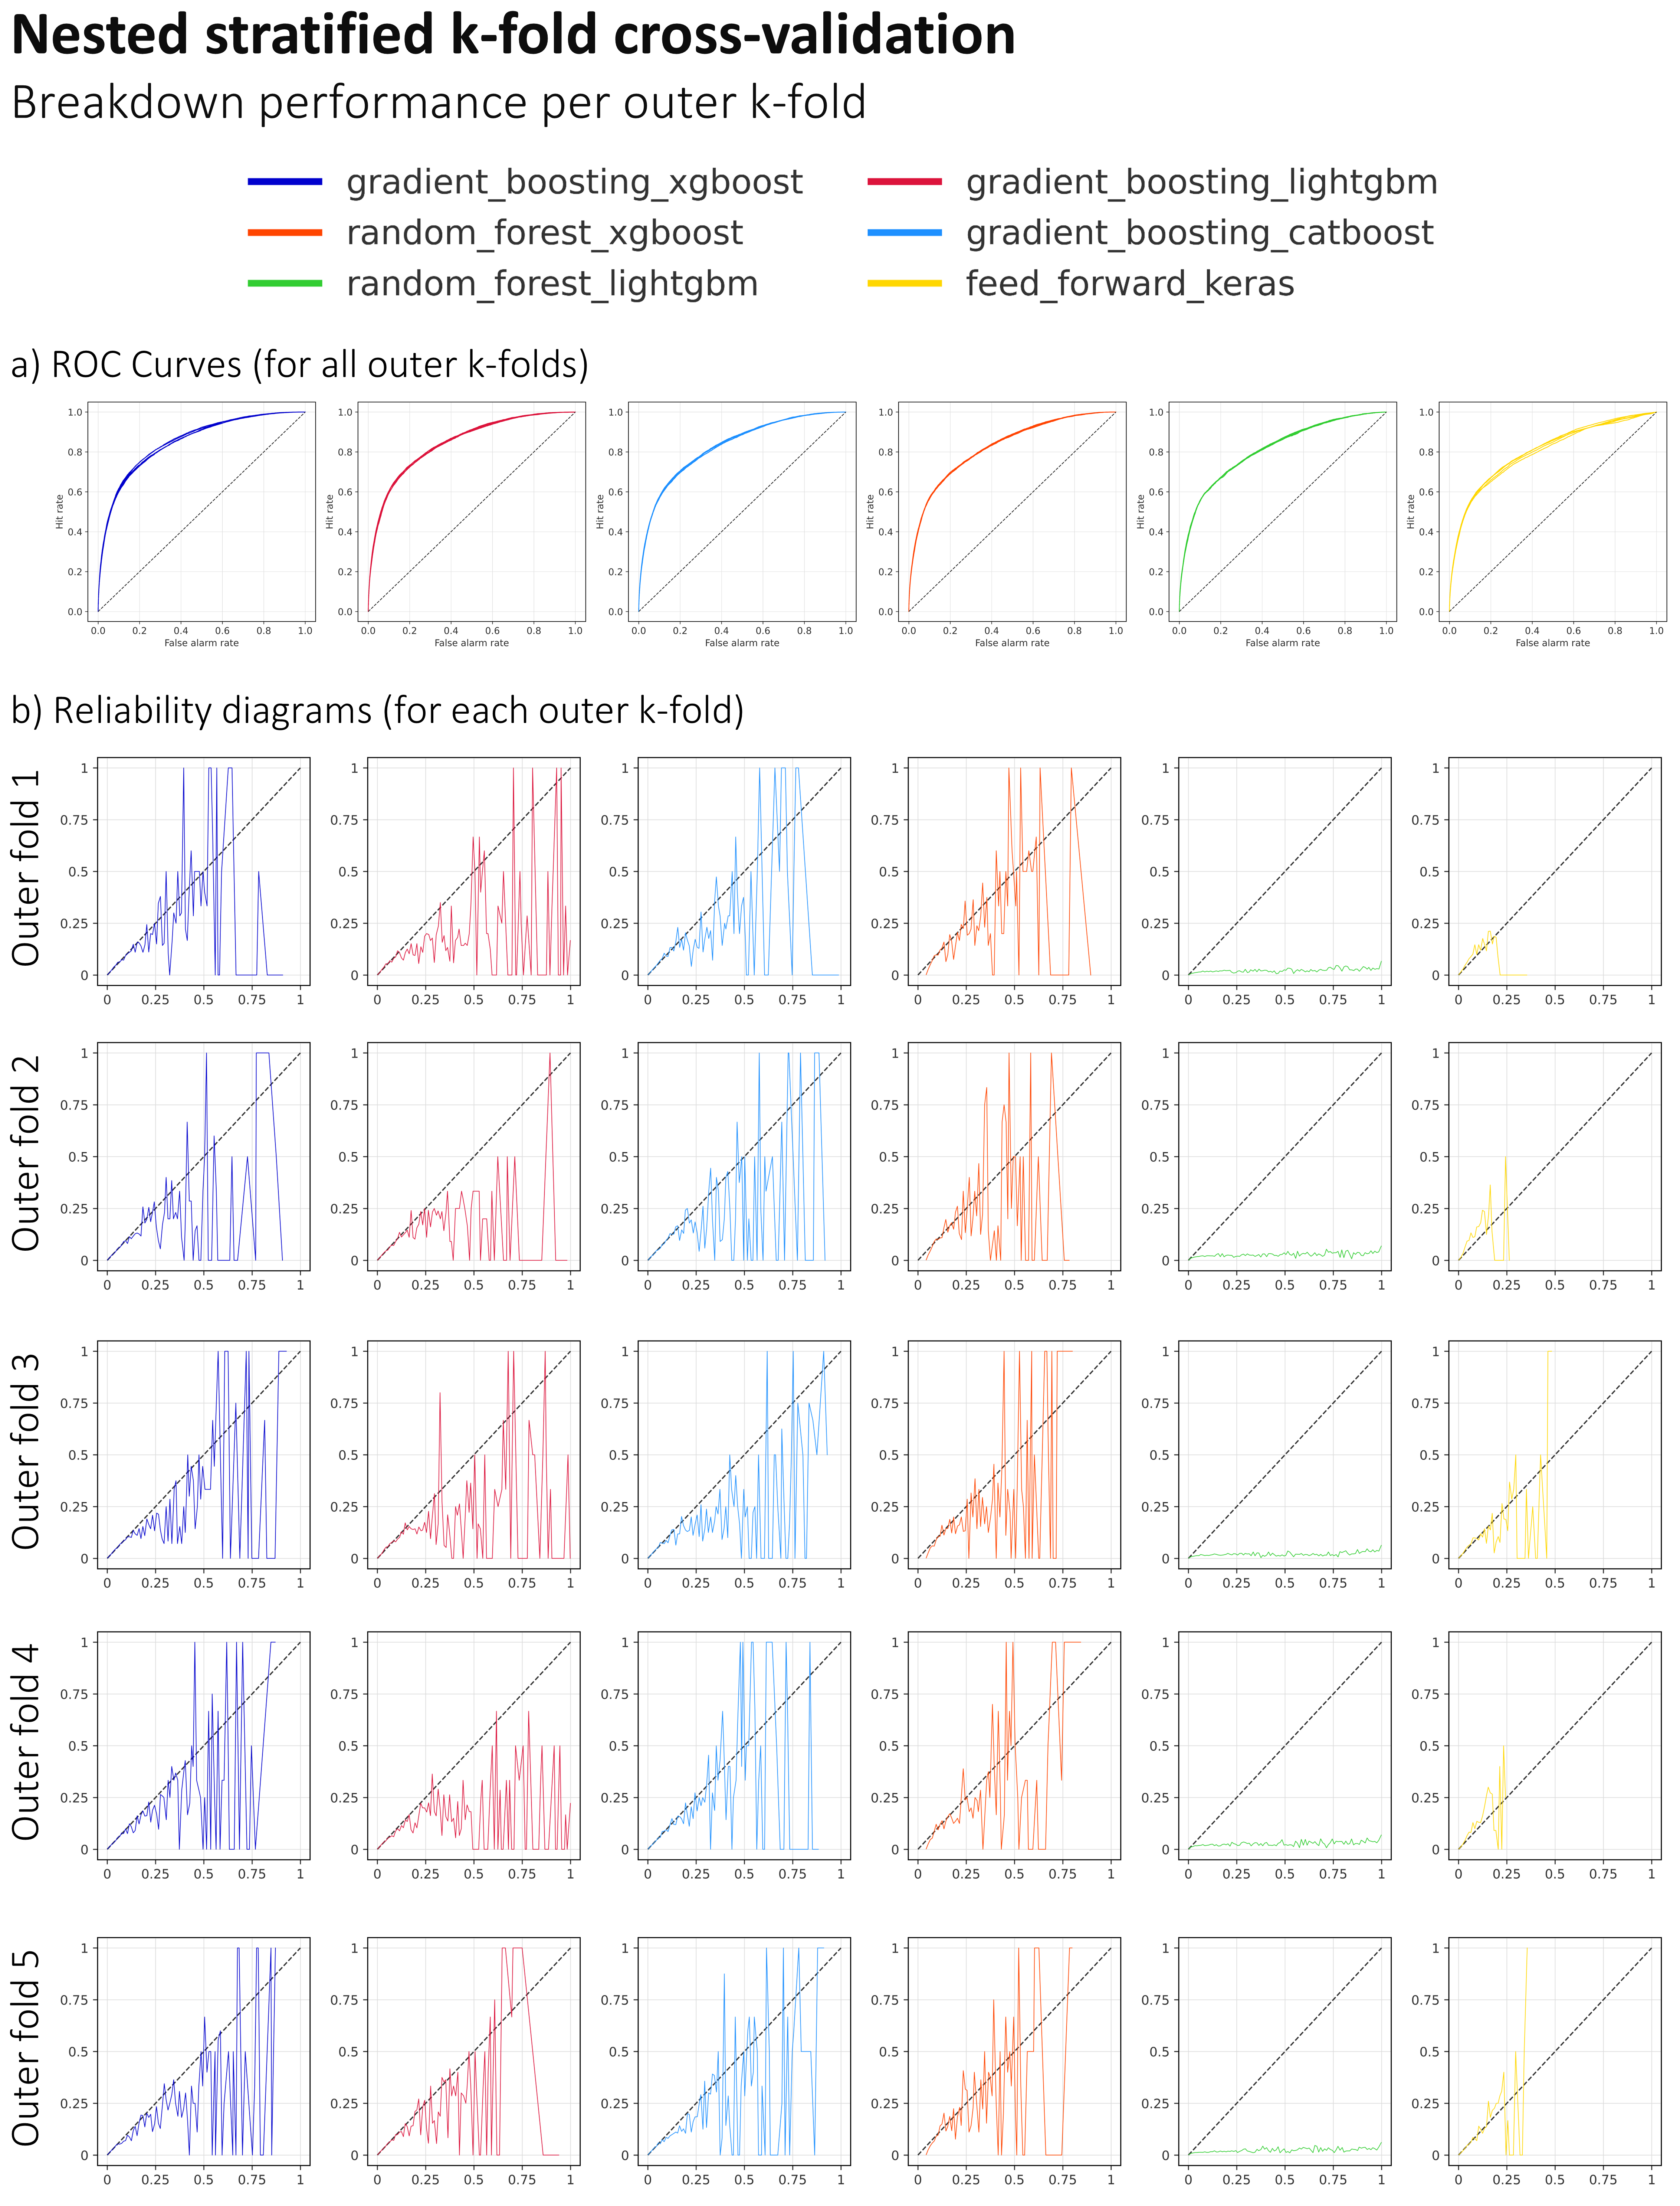
\includegraphics[width=\textwidth]{hydro_based_ff_cross_validation_optuna_breakdown_scores.png}
\caption{\textbf{Breakdown scores to estimate the model performance during the nested stratified k-fold cross validation.} Figures in panel (a) show the ROC curves for all the outer loops for gradient boosting - XGBoost implementation - in blue, gradient boosting - LightGBM implementation - in red, gradient boosting - CatBoost implementation - in cyan, random forest - XGBoost implementation - in orange, random forest - LightGBM implementation - in green, and feed forward neural network in yellow. Figures in panel (b) show the reliability diagrams for each outer loop (rows) and each model (columns).}
\label{fig:hydro_based_ff_cross_validation_optuna_breakdown_scores}
\end{figure}

In conclusion, the stability of model rankings across folds provided additional evidence of training convergence. The gradient boosting XGBoost consistently achieved the highest discrimination performance, followed closely by LightGBM, whilst the random forest implementations and neural networks occupied lower performance tiers. This consistent hierarchy across independent training runs confirms that the observed performance differences reflect genuine algorithmic characteristics rather than training artefacts or convergence failures.


\subsubsection{Final model selection}

Based on the performance metrics across all outer cross-validation folds (Figure \ref{fig:hydro_based_ff_cross_validation_optuna_overall_scores} and Figure \ref{fig:hydro_based_ff_cross_validation_optuna_breakdown_scores}, the model considered in this thesis to create the predictions of areas at risk of flash floods is the XGBoost implementation of the gradient boosting.

To establish the final model configuration for deployment (Table \ref{}), the hyperparameter values were aggregated across the outer folds using the \textit{median for continuous parameters} and the \textit{mode for categorical parameters}. This ensemble approach provided robustness against fold-specific peculiarities whilst maintaining near-optimal performance. 

\begin{table}[htbp]
\centering
\captionof{table}{\textbf{Final (optimal) configuration for the XGBoost implementation of the gradient boosting}. Values of the hyperparameters.}
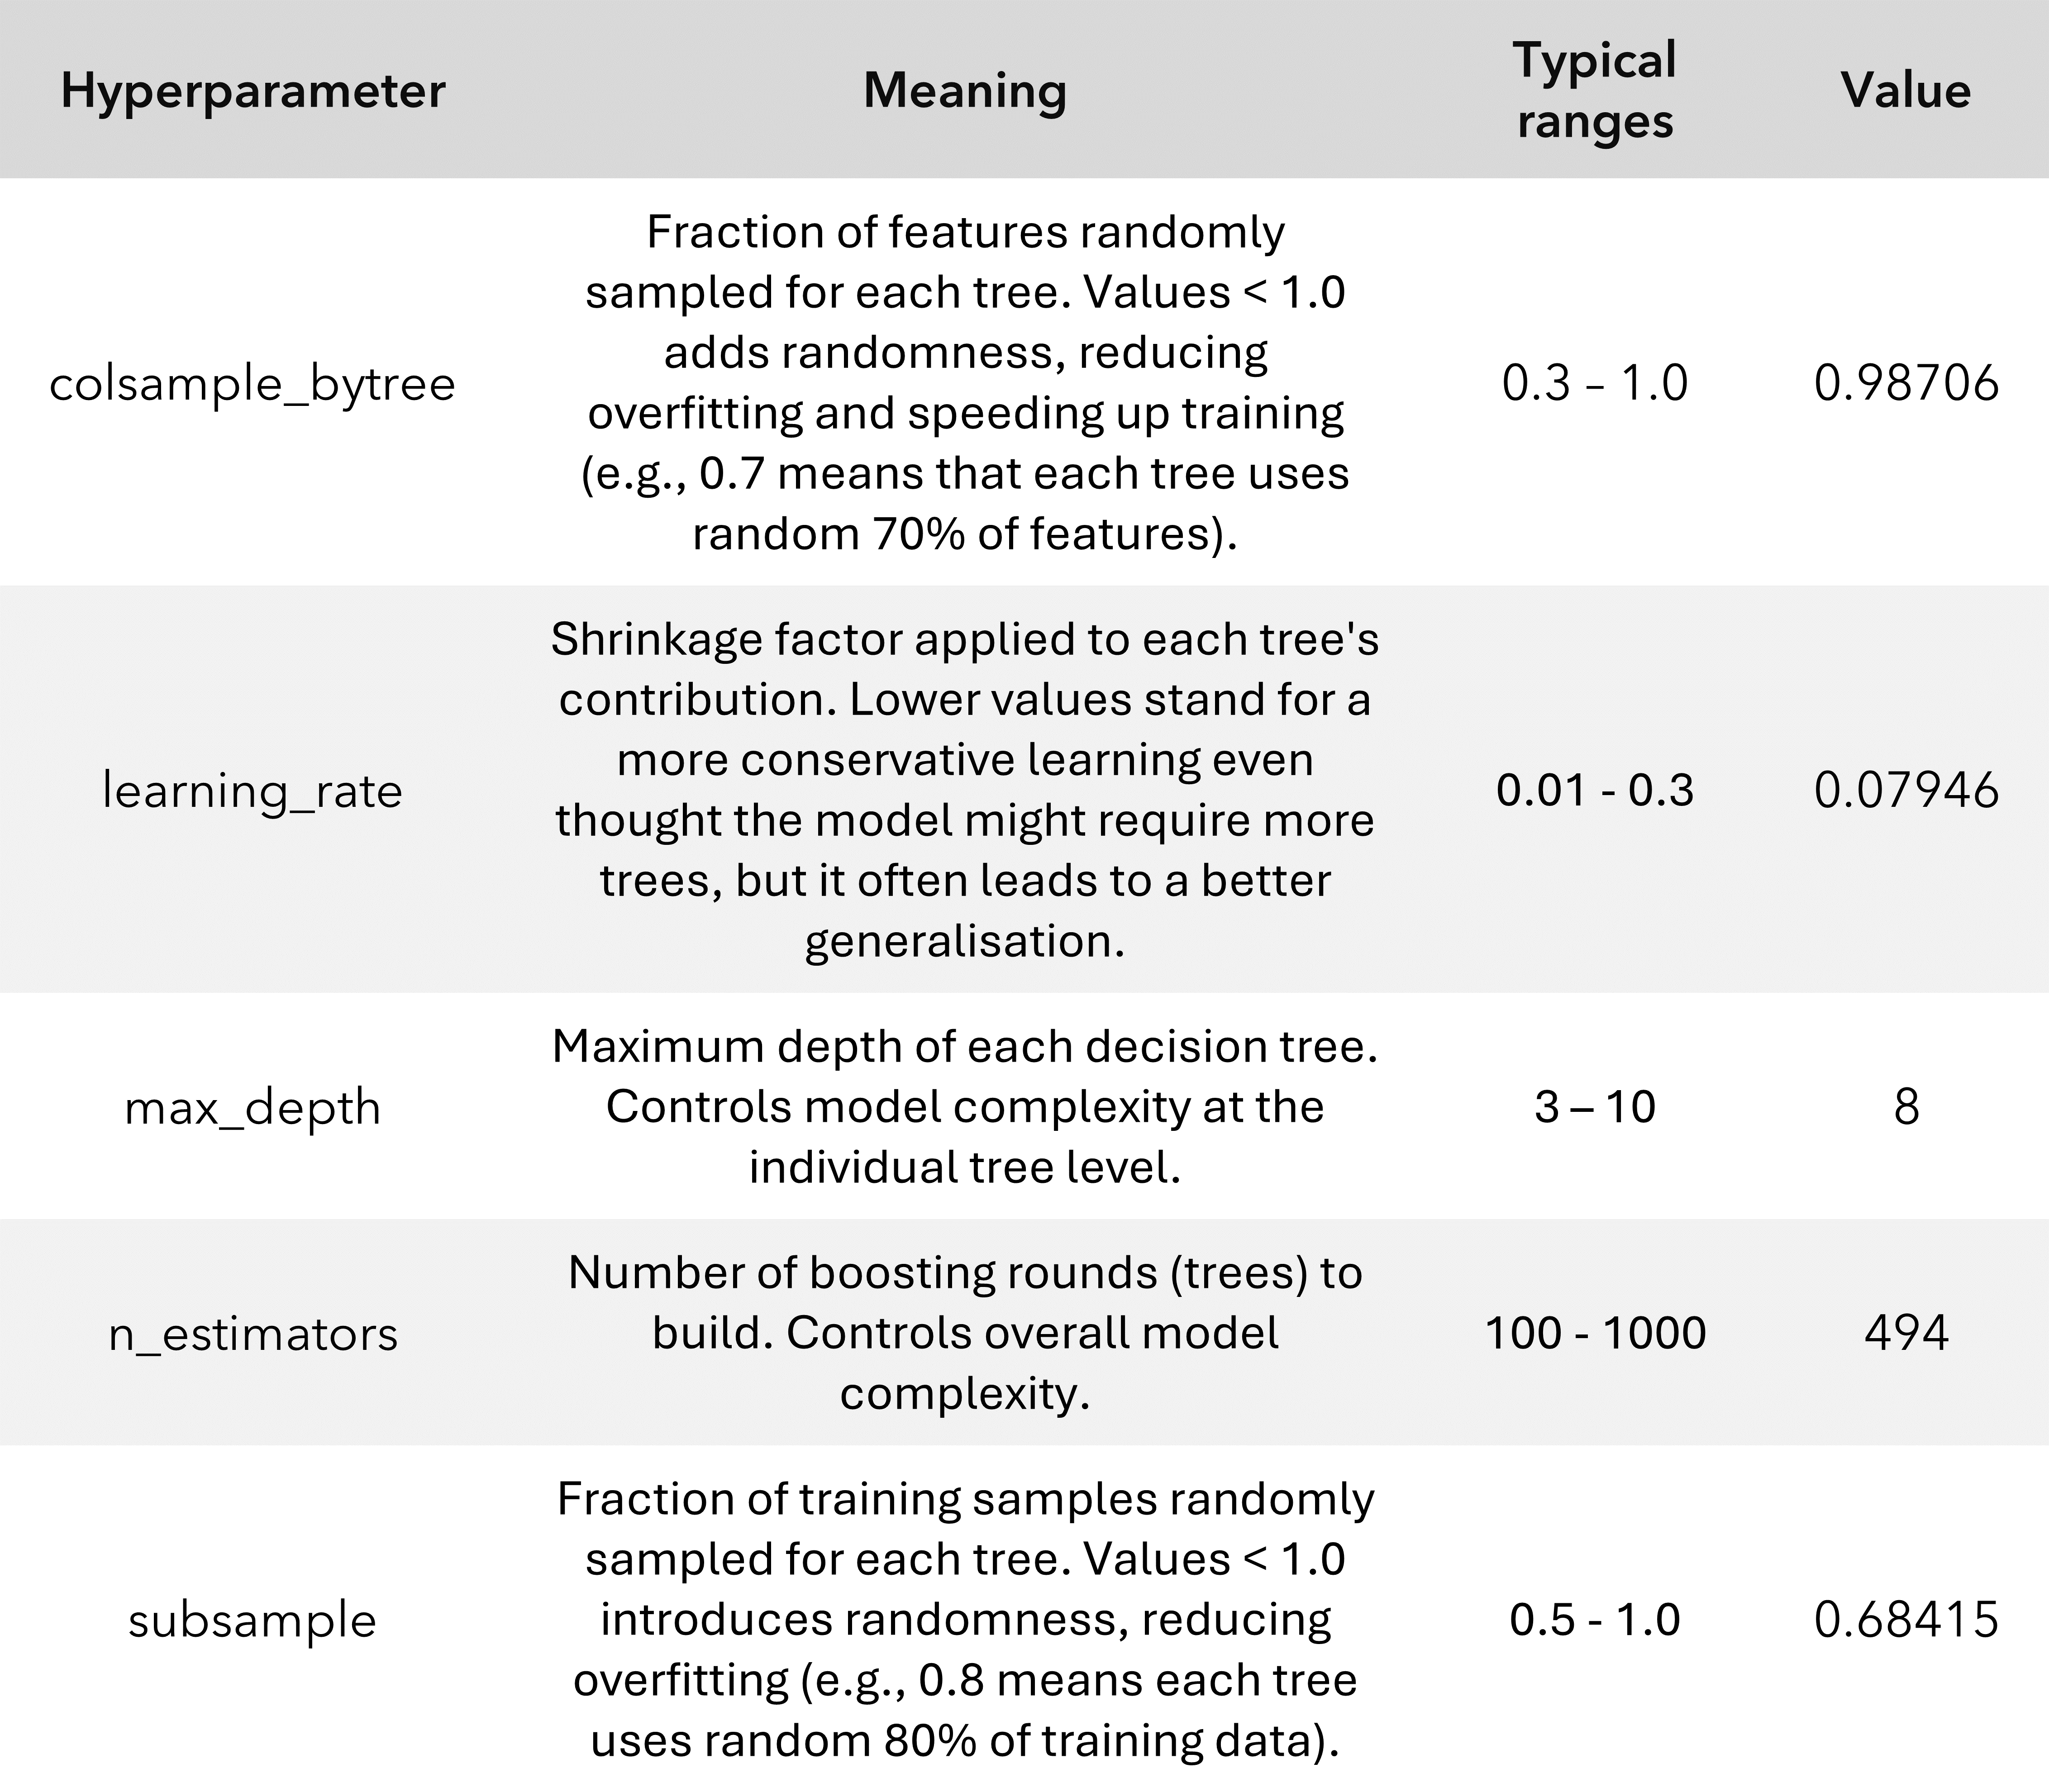
\includegraphics[width=\textwidth]{xgboost_final_configuration.png}
\label{table:xgboost_final_configuration}
\end{table}

The optimal XGBoost configuration identified through hyperparameter optimisation represents a moderately complex ensemble with careful regularisation to prevent overfitting. The model comprises 494 gradient boosted trees, each limited to a maximum depth of 8 levels, striking a balance between capturing non-linear patterns and maintaining interpretability. The learning rate of 0.07946 indicates a relatively conservative training approach, where each successive tree contributes only 7.9\% of its predictions to the ensemble, requiring the full complement of trees to achieve optimal performance whilst avoiding overshooting the loss function minima. This configuration employs substantial stochastic regularisation through both row and column subsampling: each tree is trained on a random 68.4\% of the training instances (subsample = 0.684) and utilises 98.7\% of available features (colsample\_bytree = 0.987). The high colsample\_bytree value (near 1.0) suggests that feature subsampling provides minimal regularisation benefit for this dataset, indicating that most predictors contribute meaningful information for flash flood prediction. Conversely, the moderate row subsampling (subsample = 0.68415) introduces beneficial stochasticity, helping the model generalise beyond the training data whilst maintaining sufficient data for reliable tree construction.

This configuration reflects a model that prioritises stability and generalisation over aggressive fitting, appropriate for the high-stakes nature of flash flood forecasting, where false alarms and missed events carry significant consequences. The parameter combination suggests the optimisation process favoured a large ensemble of moderately deep trees with conservative learning dynamics over a smaller set of more complex trees, likely improving the model's robustness to variations in hydro-meteorological conditions.

\subsubsection{Computation requirements}




%%%%%%%%%%%%%%%%%%%%%%%%%%%%%%%%%%%%%%%%%%%%%%%%%%%%%%%%%%%%%%%%%%%%%%%%%%%%%%%%
\subsection{Assessment of short- and long-range data-driven hydro-meteorological predictions of areas at risk of flash floods}

\subsubsection{Overall verification scores}

Figure \ref{fig:hydro_based_ff_verif_overall_scores} presents the results of the objective verification analysis carried out on the hydro-meteorological, data-driven predictions of areas at risk of flash floods. It shows distinct performance characteristics between the short-range forecasts (also known as reanalysis) and the long-range forecasts (up to t +120, day 5). It is worth noticing that day 1 forecasts (t+24) have a very similar value compared to those for day 0 (short-range) forecasts, in all verification scores. 

The area under the ROC curve (Figure \ref{fig:hydro_based_ff_verif_overall_scores}a) shows forecasts with strong discrimination ability, maintaining values above 0.75 across all lead times. The short-range forecast (lead time 0) and day 1 forecasts achieve the highest discrimination performance with an AROC of approximately 0.83, indicating excellent ability to distinguish between flash flood and non-flash flood events. As lead time increases, the AROC exhibits a gradual linear decline, reaching \sim0.77 at day 5 forecasts (\sim7\% reduction in discrimination ability from day 0). Such a small reduction, especially compared to the rainfall-based forecasts, represents a modest degradation considering the extended forecast range, suggesting that the model maintains substantial predictive skill even at longer lead times.

The frequency bias (Figure \ref{fig:hydro_based_ff_verif_overall_scores}b) reveals a dramatic shift in forecast behaviour between short-range and long-range predictions. The day 1 forecasts show nearly identical frequency bias compared to day 0 (short-range) forecasts, i.e, \sim15. From day 2 forecasts, the frequency bias starts increasing, reaching a frequency bias that doubles the one at day 1 (\sim 31) at day 4. Comparing these results to the rainfall-based forecasts, where the frequency bias remains mostly constant over the different lead times, it would not be reasonable to think that the degradation of the frequency bias in the hydro-meteorological, data-driven forecasts are mainly due to variations in skill of the soil moisture with lead time, as the other parameters adopted in the data-driven model (orography and vegetation cover, are either static or climatological).

The recall (Figure \ref{fig:hydro_based_ff_verif_overall_scores}c) and F1-score (Figure \ref{fig:hydro_based_ff_verif_overall_scores}d) show a similar pattern. The day 1 forecasts show a slightly higher value compared to the one at day 0 (\sim 0.11 for recall and 0.08 for F1-score). From day 2, both scores half around day 5. This means that, according to both metrics, the model's ability to detect true positives deteriorates significantly beyond day 2, with the 5-day forecast detecting \sim half the events identified by the short-range forecast or the day 1 forecasts.

These verification metrics collectively indicate that the data-driven approach performs optimally at 0-1 day lead times, with acceptable performance extending to day 2. Beyond this threshold, whilst discrimination ability (AROC) remains reasonable, the operational utility diminishes substantially due to excessive false alarm rates and reduced detection capability, suggesting to further adjust the lead-time-dependent probability thresholds or alternative modelling strategies for extended-range flash flood forecasting.


\begin{figure}[htbp]
\centering
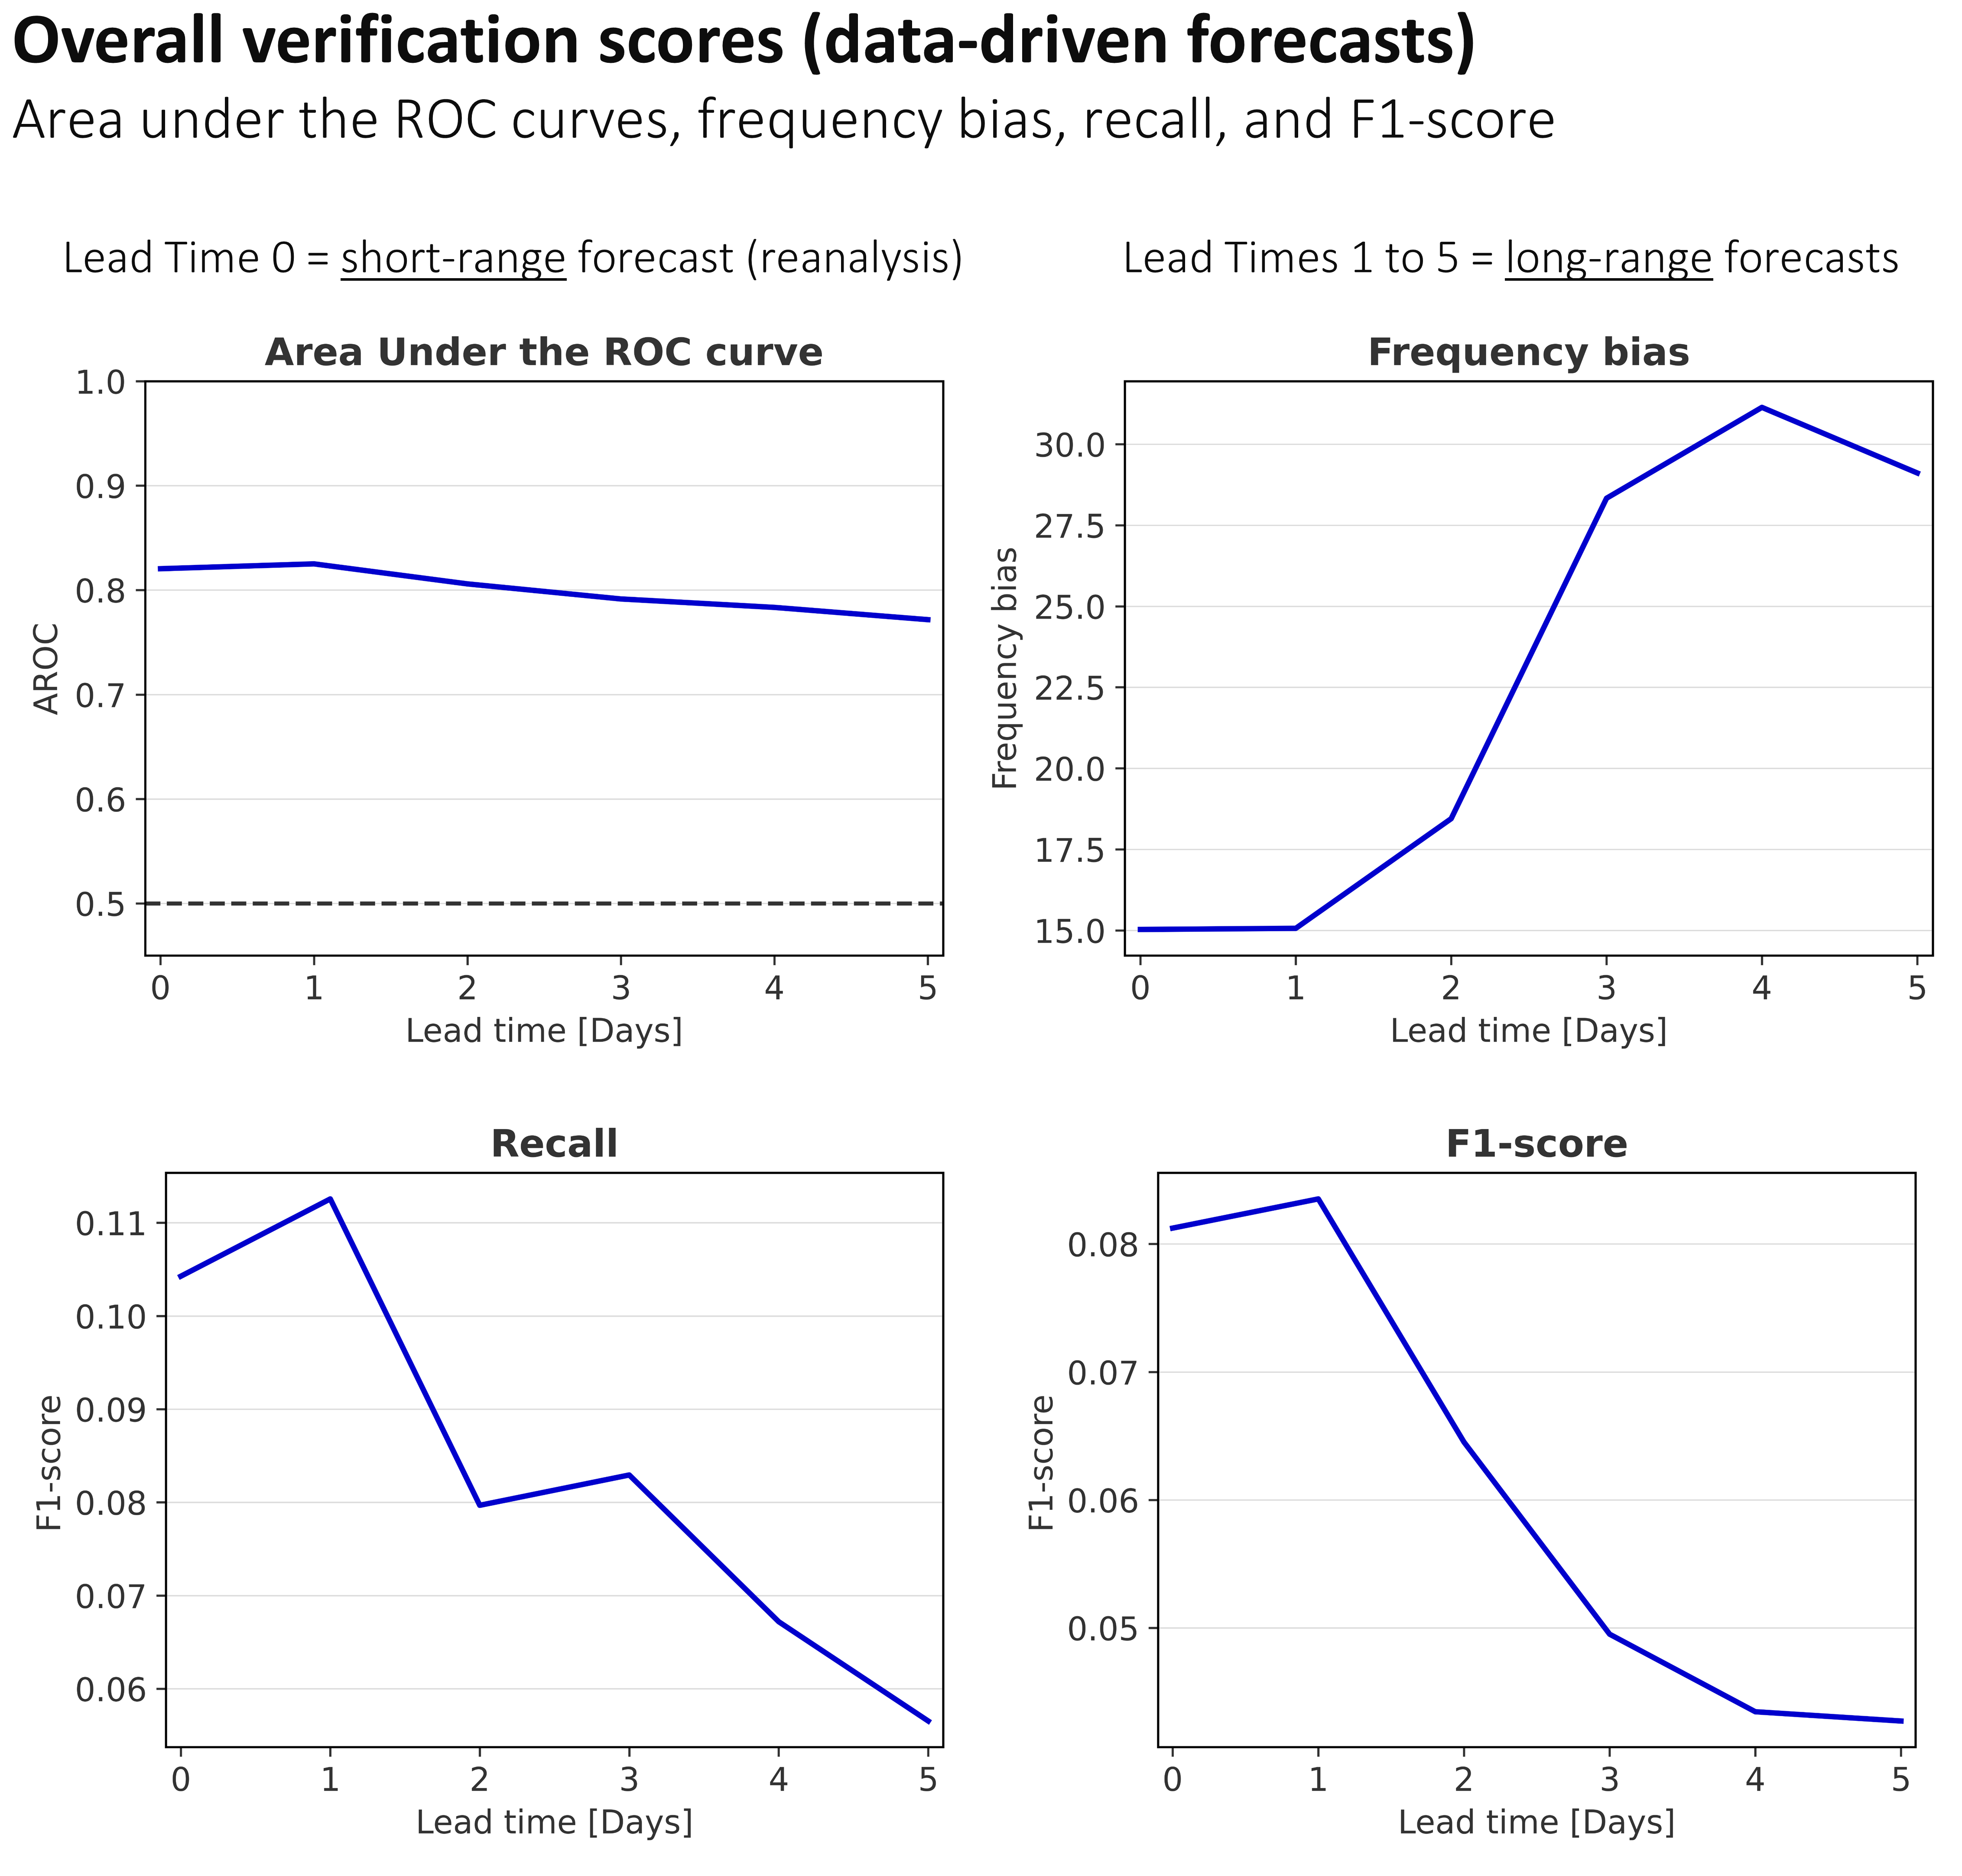
\includegraphics[width=\textwidth]{hydro_based_ff_verif_overall_scores.png}
\caption{\textbf{Overall verification scores for data-driven, hydro-meteorological forecasts.} Panel (a) shows the Area under the ROC curve for the short-range forecasts (i.e., reanalysis, lead time = 0), and the long-range forecasts (lead time = 1 - t+24, lead time = 2 - t+48, lead time = 3 - t+72, lead time = 4, t+96, lead time = 5, t+120). Panels (b) to (c) show, respectively, the frequency bias, the recall, and the F1-score.}
\label{fig:hydro_based_ff_verif_overall_scores}
\end{figure}


\subsubsection{Breakdown verification scores}

As seen in the overall verification scores, also the ROC curve for a day 1 (Figure \ref{fig:hydro_based_ff_verif_breakdown_scores_roc}, dashed line) forecast is nearly identical (almost perfect overlap) with day 0 forecasts (\ref{fig:hydro_based_ff_verif_breakdown_scores_roc}, solid and thicker line). Then, there is a small and gradual worsening of the ROC for longer-range forecasts observed by the flattening of the ROC curves towards the diagram's diagonal. Such flattening means that for a similar hit rate, the false alarms increase slightly, around 0.1.

\begin{figure}[htbp]
\centering
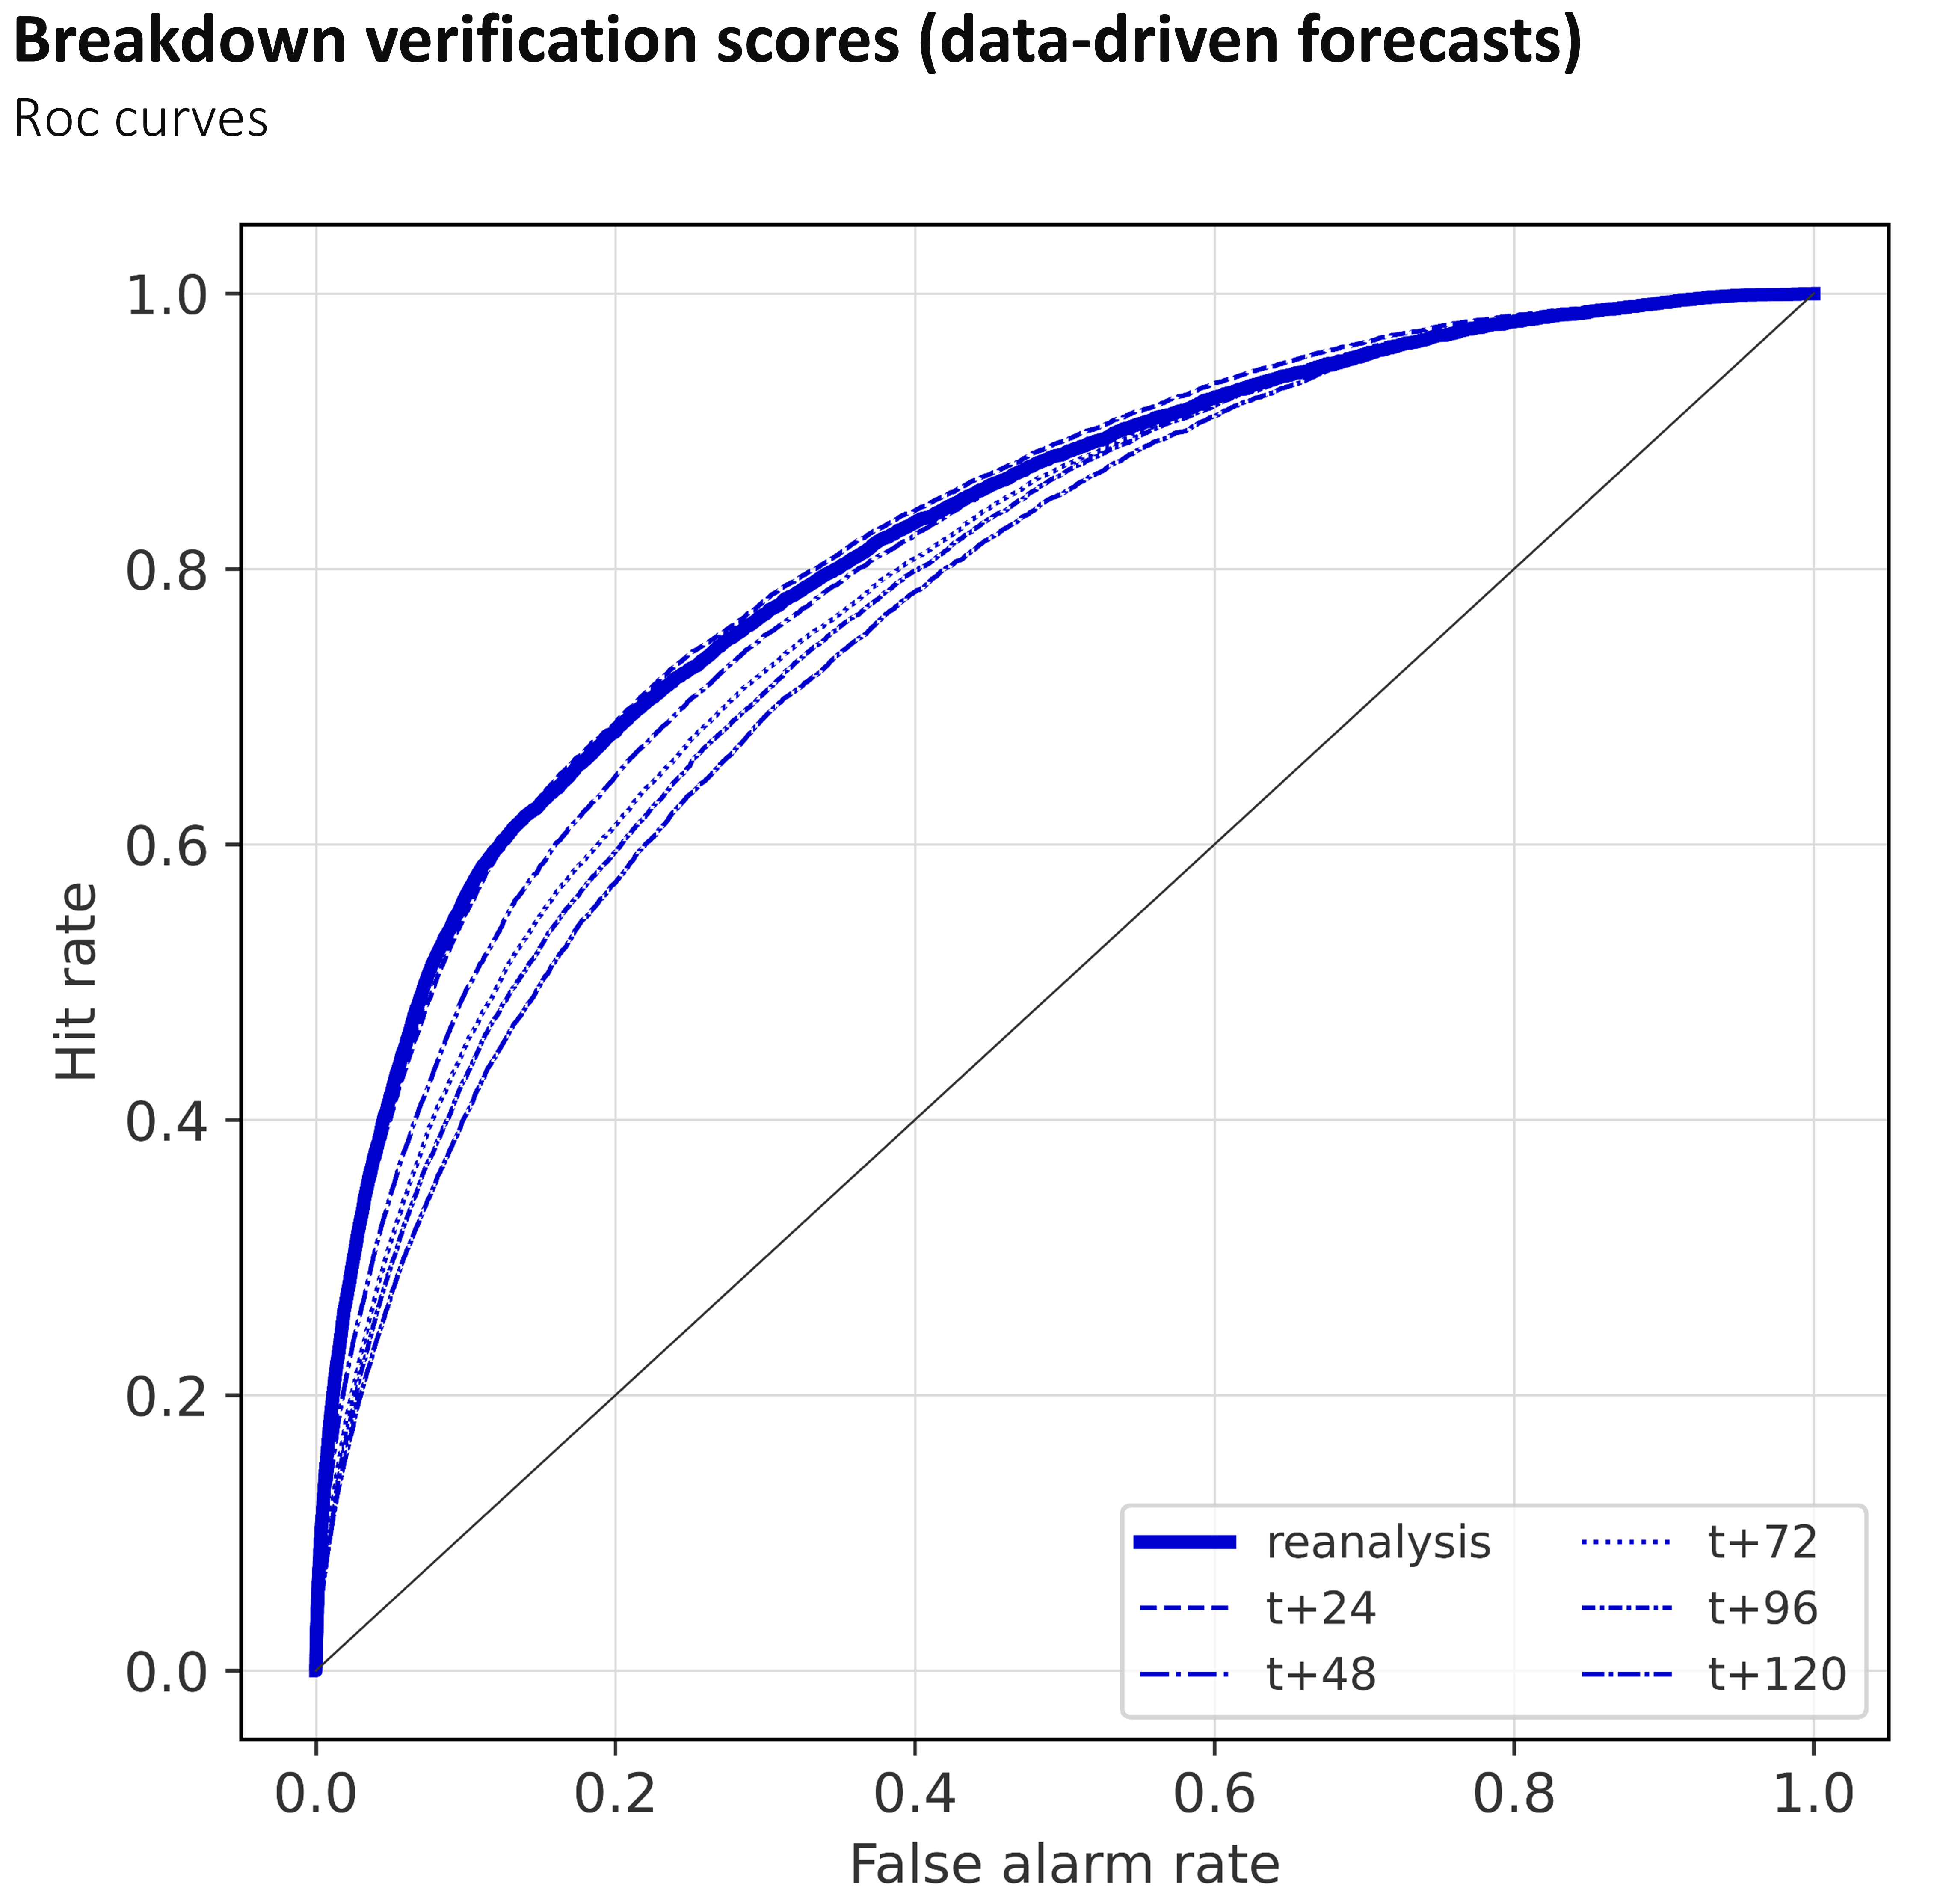
\includegraphics[width=\textwidth]{hydro_based_ff_verif_breakdown_scores_roc.png}
\caption{\textbf{Breakdown verification scores for data-driven, hydro-meteorological forecasts - ROC curves} Panels (a) to (f) show the ROC curves, respectively, for the short-range forecasts (i.e., reanalysis), for the long range forecasts at t+24 (day 1), t+48 (day 2), t+72 (day 3), t+96 (day 4), and t+120 (day 5).}
\label{fig:hydro_based_ff_verif_breakdown_scores_roc}
\end{figure}

From the reliability diagrams (Figure \ref{fig:hydro_based_ff_verif_breakdown_scores_rel_diag}) it is possible to understand better why the frequency bias increases significantly with the lead time \ref{fig:hydro_based_ff_verif_overall_scores}b. The reliability diagrams for day 0 (\ref{fig:hydro_based_ff_verif_breakdown_scores_rel_diag}a) and for day 1 (\ref{fig:hydro_based_ff_verif_breakdown_scores_rel_diag}b) are very similar. However, day 0 reliability shows a wider range of probabilities (up to \sim 15\%) with predicted probabilities similar to those observed than day 1 (with probabilities with this similar behaviour only up to \sim 10\%). At day 2 forecasts, the range of well calibrated probabilities diminishes up to 5\%, and from day 3, the predictions show mostly overestimation of the observed frequencies from forecasts probabilities exceeding 1\%. It is worth noticing how, also in the case of the rainfall-based forecasts, also the data-driven forecasts do not show a reduction of the issued probabilities with increasing lead times. As discussed in relevant section, this is due to the fact that we are using a rainfall forecasts that post-processed a deterministic system.

\begin{figure}[htbp]
\centering
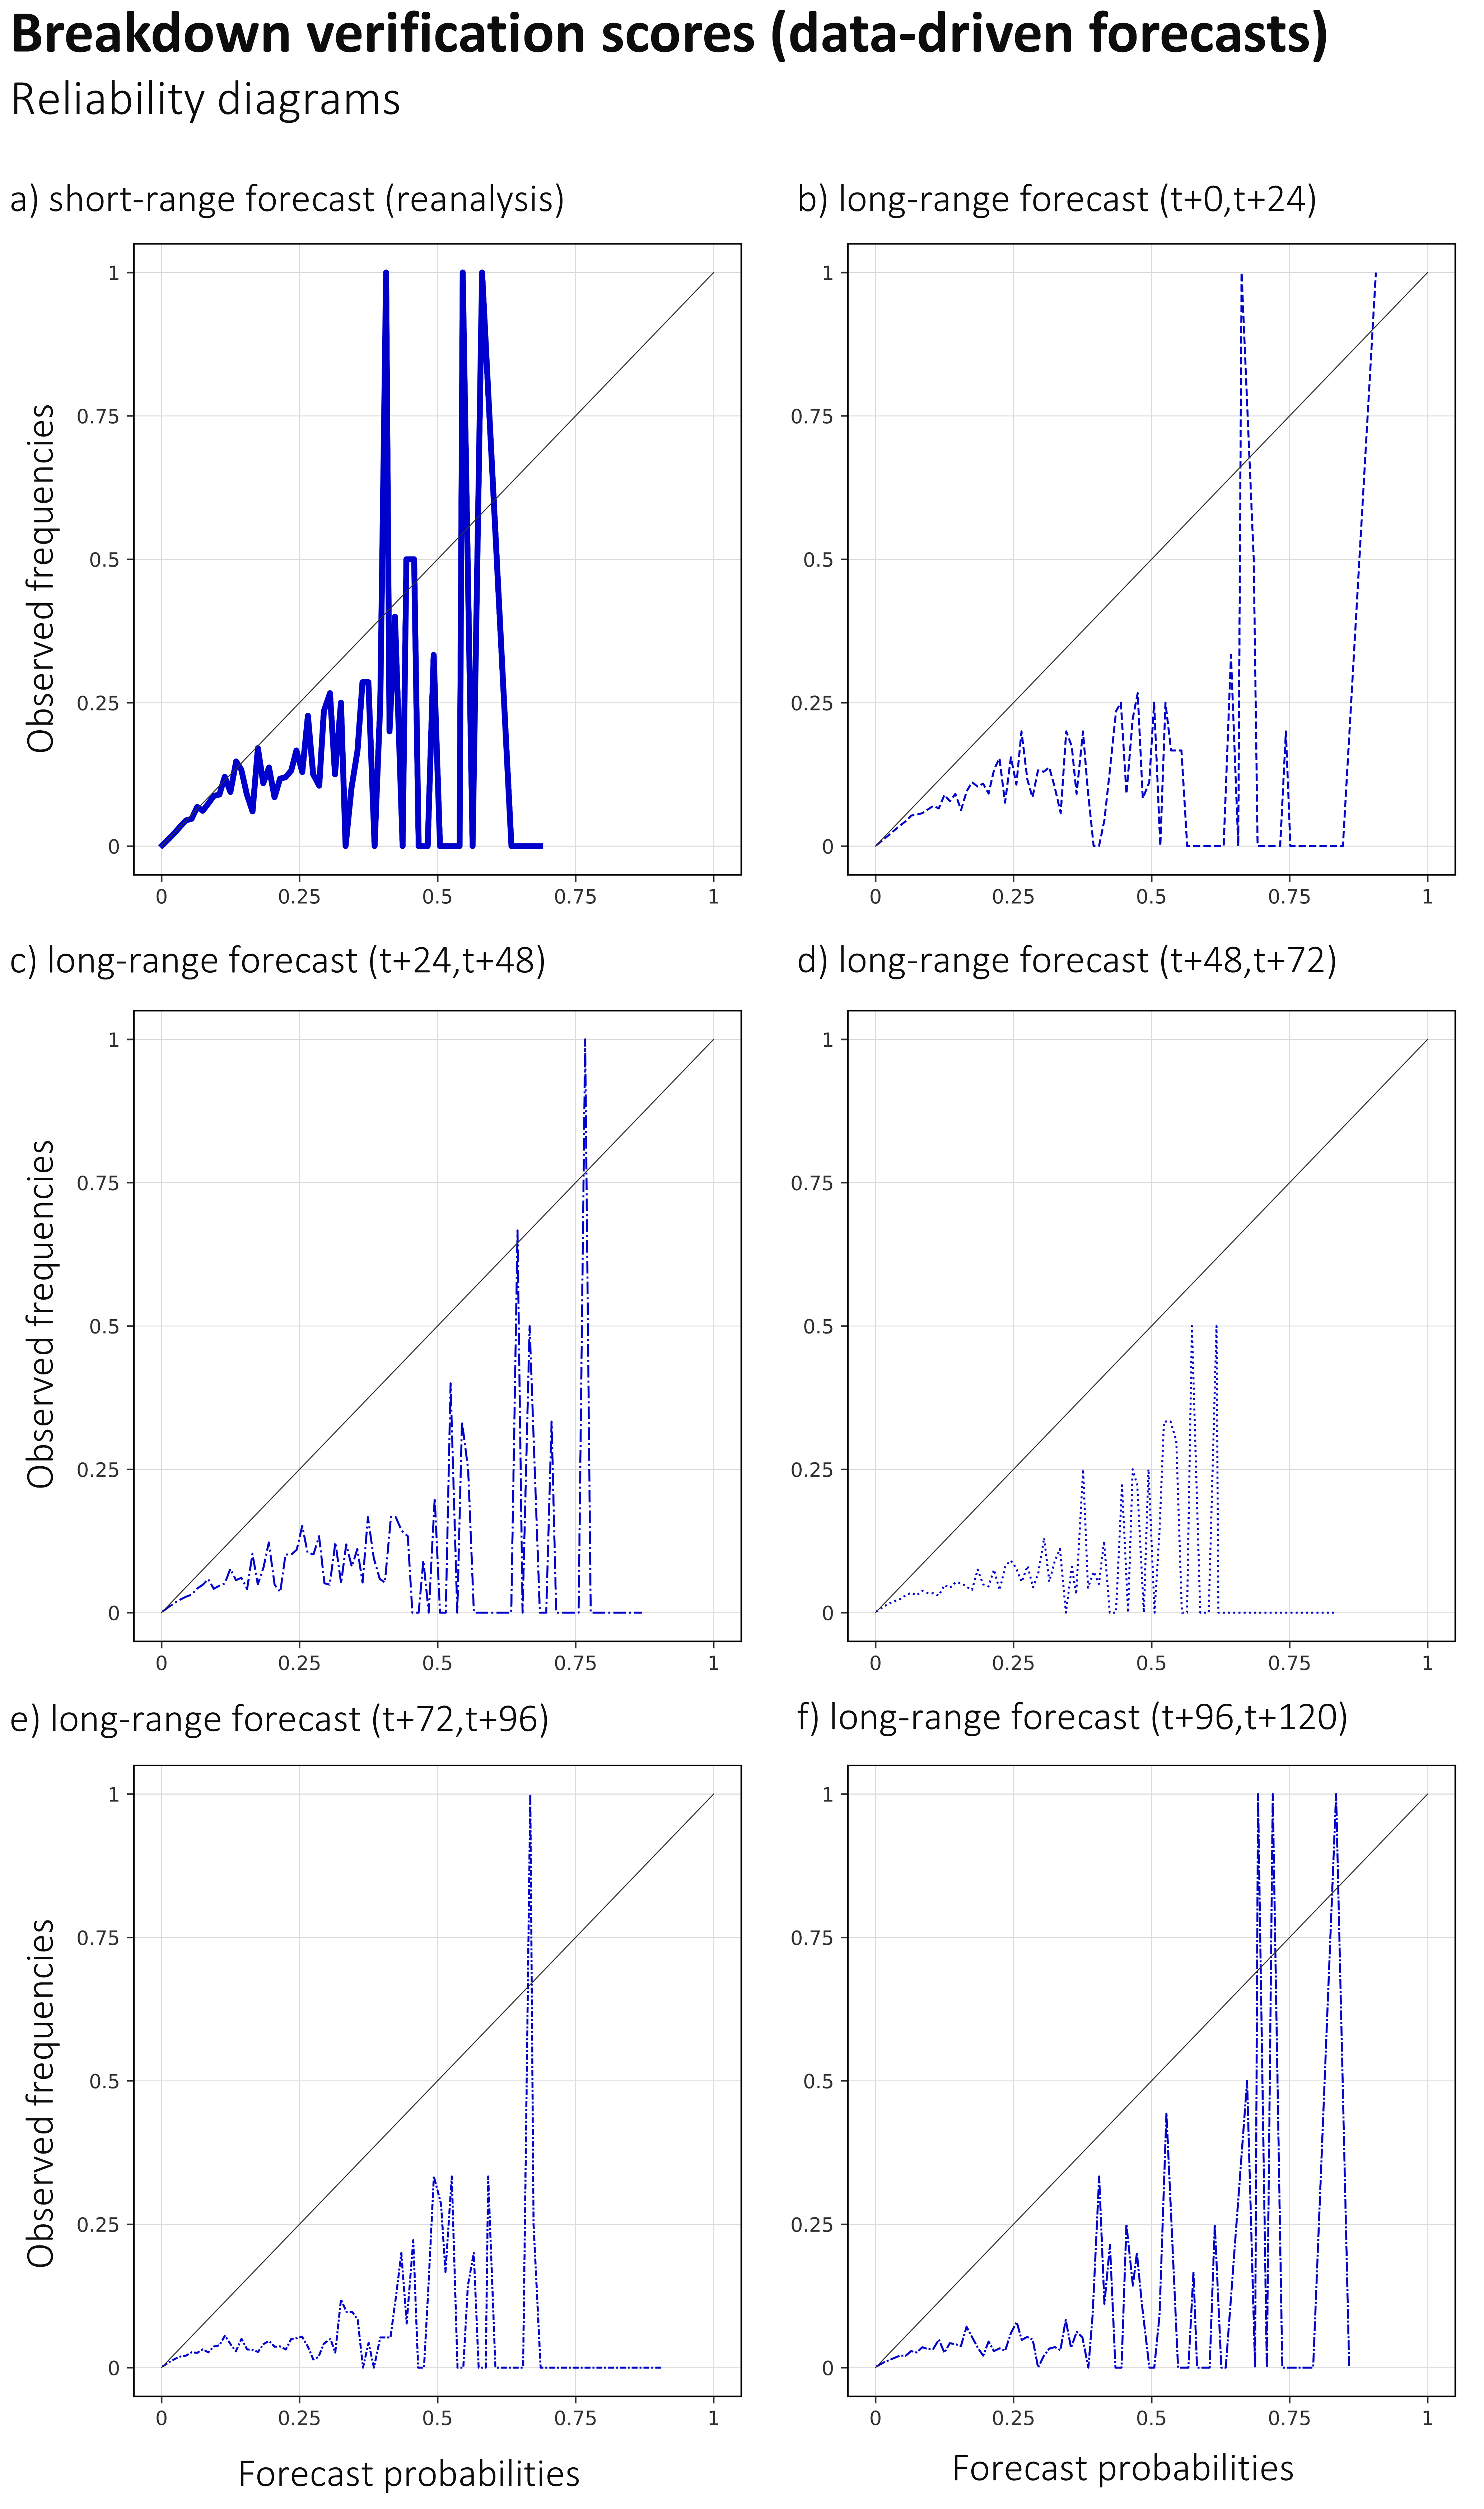
\includegraphics[width=\textwidth]{hydro_based_ff_verif_breakdown_scores_rel_diag.png}
\caption{\textbf{Breakdown verification scores for data-driven, hydro-meteorological forecasts - Reliability diagrams} Panels (a) to (f) show the reliability diagrams, respectively, for the short-range forecasts (i.e., reanalysis), for the long range forecasts at t+24 (day 1), t+48 (day 2), t+72 (day 3), t+96 (day 4), and t+120 (day 5).}
\label{fig:hydro_based_ff_verif_breakdown_scores_rel_diag}
\end{figure}


%%%%%%%%%%%%%%%%%%%%%%%%%%%%%%%%%%%%%%%%%%%%%%%%%%%%%%%%%%%%%%%%%%%%%%%
\subsection{Physical interpretation of the data-driven model behaviour}



\subsection{Extension of regional training to global application}

\begin{figure}[htbp]
\centering
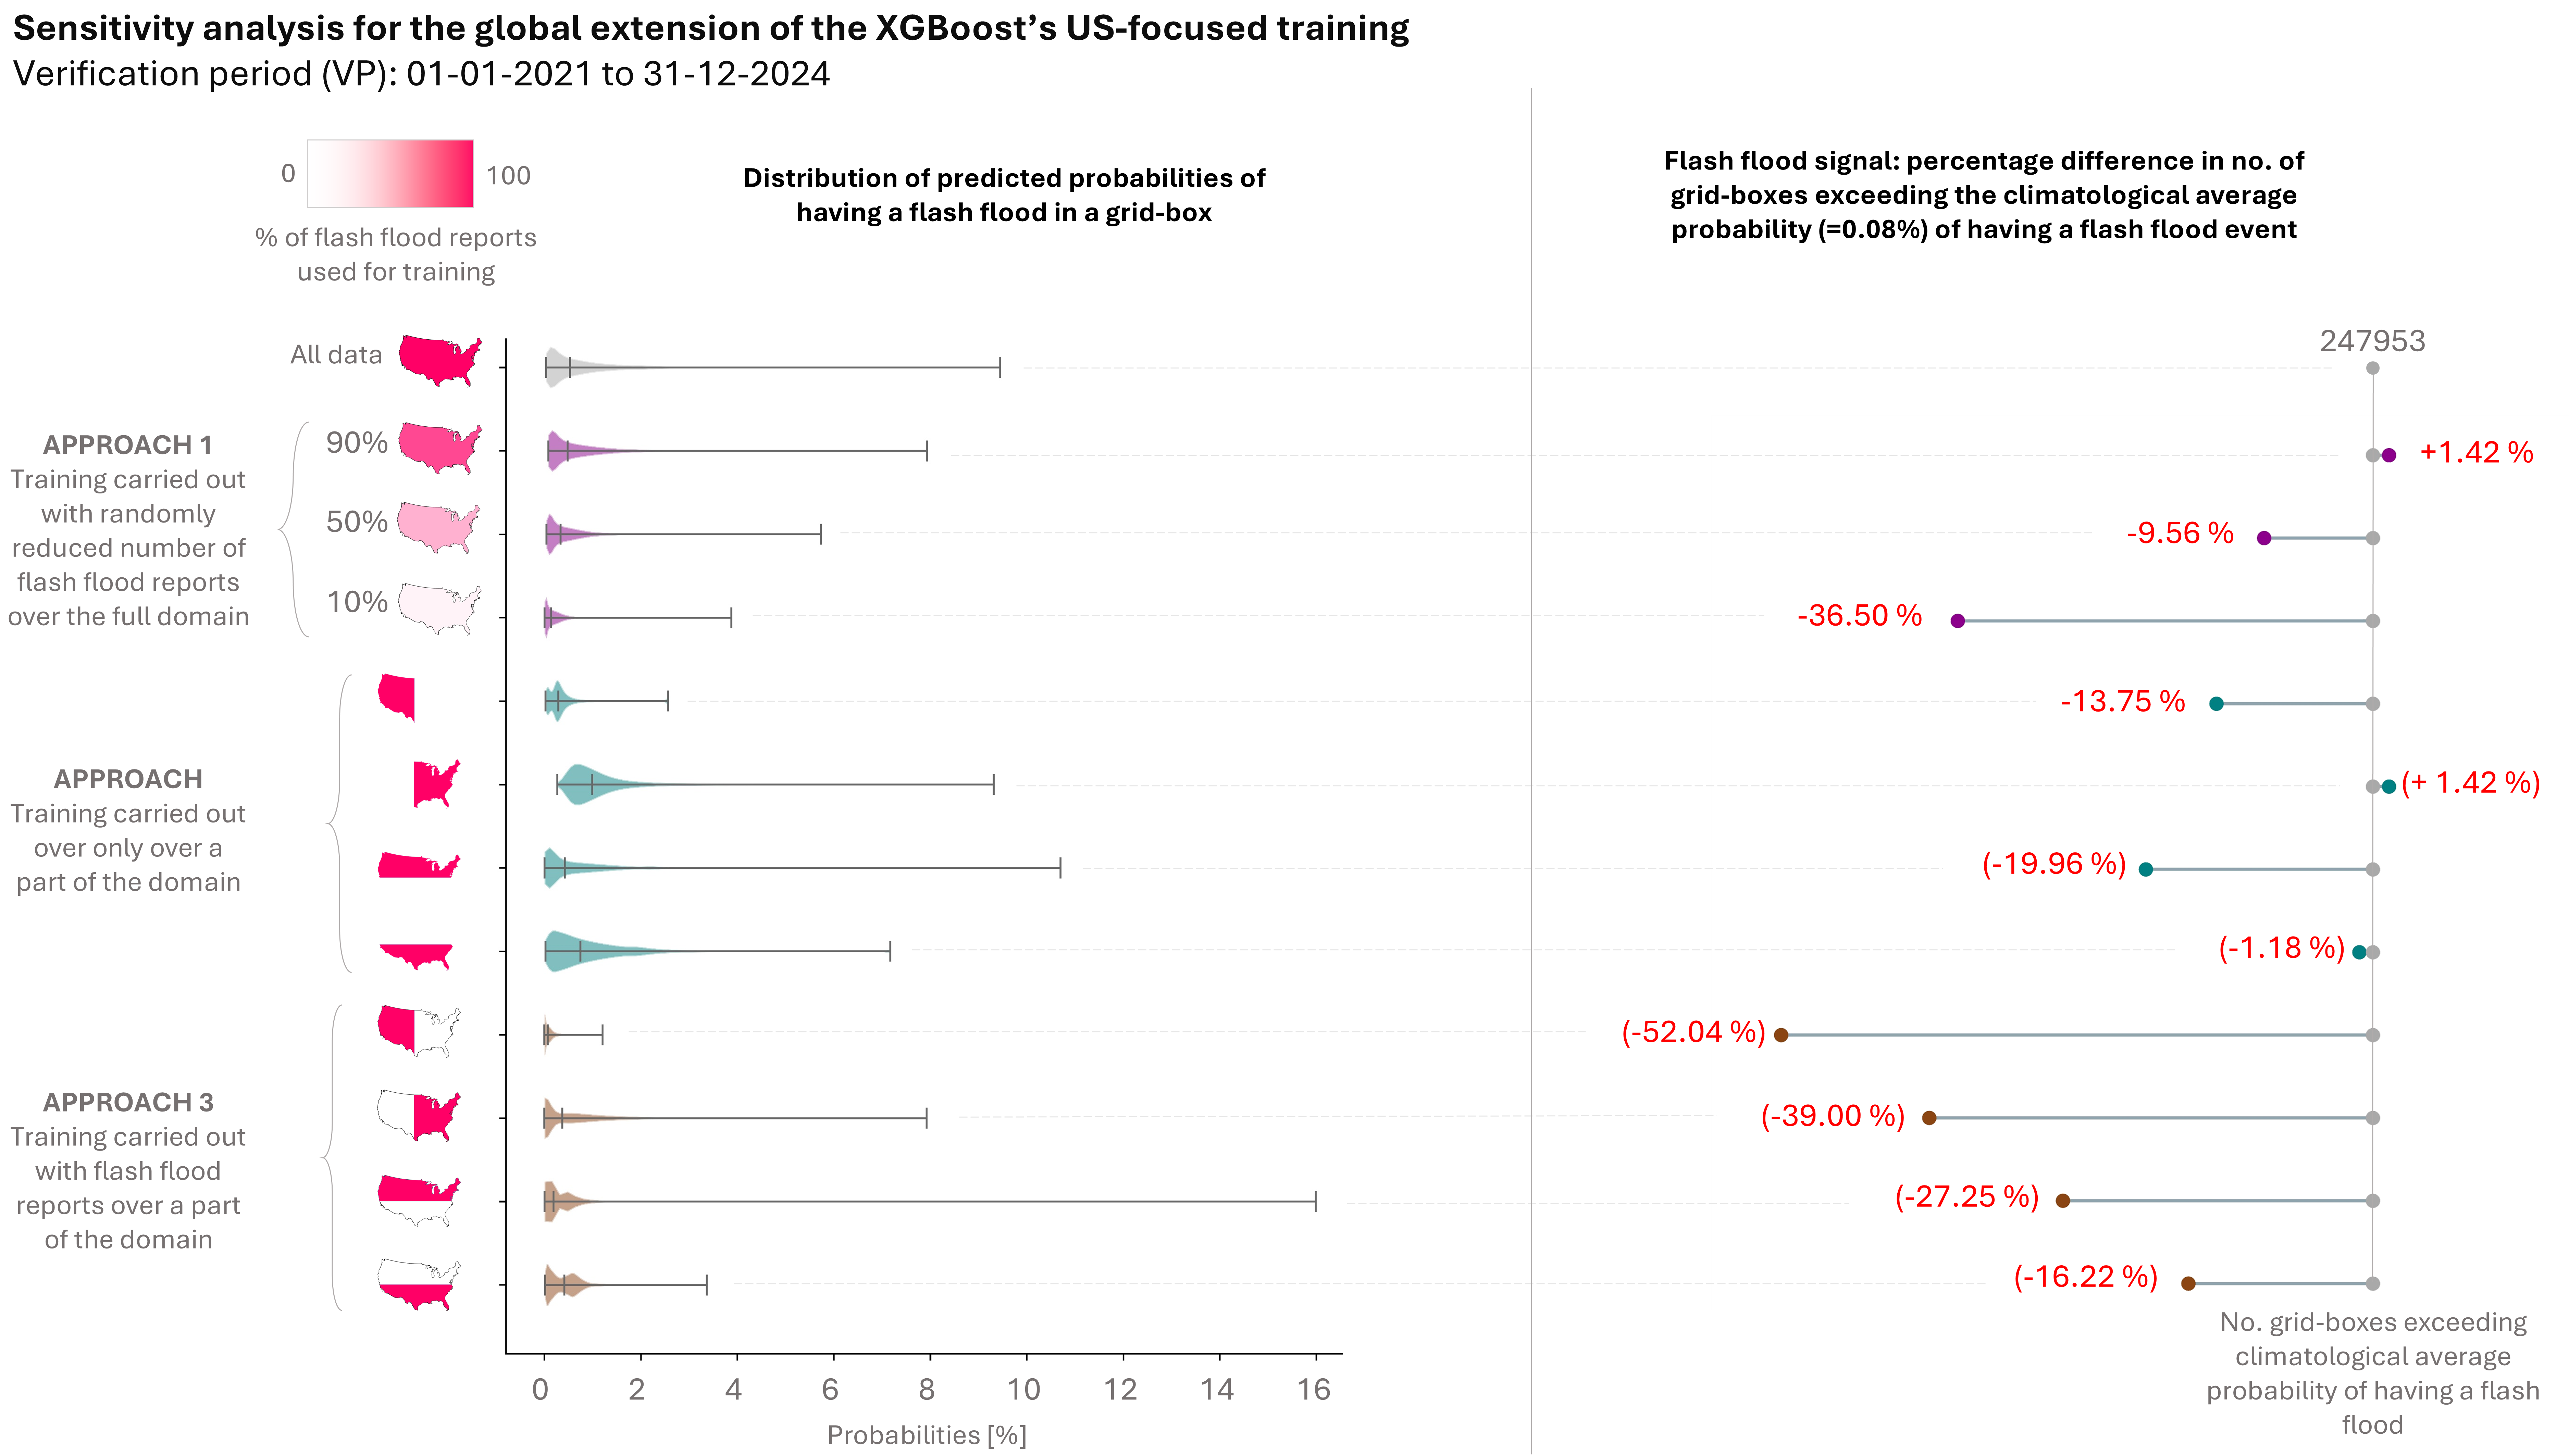
\includegraphics[width=\textwidth]{sensitivity_analysis_global_extension.png}
\caption{\textbf{Global extension performance of regionally-trained XGBoost under different U.S. training data sampling strategies.} Violin plots show predicted probability distributions, whilst dots indicate percentage change in flash flood detection capability relative to climatological baseline. Three approaches tested: random sampling (Approach 1), domain-restricted training (Approach 2), and sub-regional training (Approach 3).}
\label{fig:sensitivity_analysis_global_extension}
\end{figure}

The global application of the regionally-trained XGBoost was evaluated through three distinct approaches, each employing different spatial sampling strategies for training data inclusion (Figure \ref{fig:sensitivity_analysis_global_extension}). The baseline configuration utilising all available flash flood reports in the Storm Event Database, within the verification period, produced a conservative probability distribution, with most predictions remaining below 10\% and 247,953 grid boxes exceeding the climatological average flash flood probability (0.08\%).

Approach 1, which implemented a random reduction of the flash flood reports to predetermined percentages (90\%, 50\%, and 10\%) uniformly, across the entire U.S. domain, demonstrated variable performance. The 90\% sampling configuration merginally increased the detection capability (i.e. number of flash flood reports exceeding the climatological average of flash flood events) by 1.42\%, while the 50\% and the 90\% reductions showed, respectively, a degradation of 9.56\% and 36.50\%, suggesting non-linear relationships between training data volumes and model performance.

Approach 2 explored a spatially-constrained training strategy where the model was trained only over a certain part of the domain where observations are available. The model did not see at all the other part of the domain, and it was applied to create predictions over the whole CONUS domain. This approach simulates a global training that considers only those areas of the world with good observations during training, but uses the model globally to create predictions over the continuous global domain. The reduction in the predicted probabilities was the smallest over the three approaches, with the biggest  reductions of -13.75\% and -19.96\% when the model was trained using the parts of the domain with the smallest number of flash flood reports i.e., the east and the north, respectively. When using the parts of the domain with the biggest number of reports, i.e., the west and the south, there was an increase of +1.42\% and a minimal reduction of -1.18\% of grid-boxes with a flash flood signal.

Approach 3 explores a similar spatially constrained training, where the model is trained over the whole CONUS but with observations only over a restricted part of the domain. This approach simulates a global training of the model over the whole global domain, and considering all available reports. This is the approach with the biggest reduction in predictive ability, with reductions ranging from -52.04\% when the east side was considered and -16.22\% when the south was considered, where training data is most geographically limited.

The varying performance across different training strategies highlights the critical importance of training data representativeness for successful global model deployment. These results show that the distribution of predicted probabilities and the predictive capabilities do change for different data reduction strategies. In all cases, the probability distributions remain highly skewed towards zero probabilities. Such high concentration near the zero value does not surprise as flash floods are rare events. However, the shape and the spread of the probability values varies greatly, with more compressed distributions (with probability values rarely exceeding 2\%) over those cases that train the model with very little training data (cases 4, 5, and 9). Such compression of the probability distribution suggests that the model becomes increasingly conservative and uncertain with less data. When training instead over regions with higher training data volumes (cases 1, 6, 8, 10, and 12), the model seems to be more willing to predict moderate-to-high probabilities. The shape of the distributions is also important. Overall, the shape does not change compared to the baseline (grey violin plot, case 0) with the training approach 1, while the shapes change for approach 2 and 3. The "bulges" in the middle of the distributions, primarily in approach 2, but also in approach 3 suggest the model learned to produce intermediate probabilities (2-6\%), indicating the model developed a more nuanced risk stratification, without losing the capability to predict larger probabilities unless the training dataset is very poor, as in case 5 and 9 represented by the west coast of the CONUS (the area with the least number of flash flood reports over the CONUS). 

The application of these three training strategies suggest that while global applications can maintain reasonable performance under certain conditions, data volumes play a crucial role in determining the transferability of regional flash flood forecasting models to global applications. Due to the presented results, approach 2 is selected for the global application of the CONUS-focused training, i.e., the regional training over the CONUS, using only the Storm Event Database, is applied to global fields to create predictions of areas at risk of flash floods over a continuous global domain. While it is not possible to run a robust verification analysis over the whole global domain due to the sparse density of global datasets like EM-DAT and DesInventar, section \ref{verif_case_study} will provide a selection of case studies over the CONUS and around the world to examine the performance of the regional and global training.


%%%%%%%%%
\section{Catalogue of flash flood events}
\label{verif_case_study}